\documentclass[english,11pt]{article}

\usepackage{helvet}
\usepackage{times}
\usepackage{a4wide}
\usepackage{latexsym}
\usepackage{babel}
\usepackage{rotating}
\usepackage{float}
\usepackage{calc}
\usepackage{fancyhdr}
\usepackage{lastpage}
\usepackage{epsfig}
\usepackage{longtable}
\usepackage{multirow}
\usepackage{wrapfig}
\usepackage{subfigure}
\usepackage{gensymb}

\usepackage{euproposal}

\usepackage[a4paper, top=20mm, bottom=20mm, left=20mm, right=20mm]{geometry}
\usepackage{natbib}
\setlength{\bibsep}{0pt plus 0.3ex}


%CP: remove that for final version?
\usepackage[linkcolor=blue,colorlinks=true]{hyperref}

\newcommand{\svnrevision}{PDF generated on \today{}}
%%\include{svnrevision}

\newcommand{\stepcounterarabic}[1]{\stepcounter{#1}\arabic{#1}}

%\newcommand{\captionfont}{\small \it}
\usepackage[font={small,it}]{caption}
\usepackage[right]{eurosym}

\usepackage[T1]{fontenc}

\usepackage{wrapfig,graphicx}
\usepackage{url}

%%---------------------------------------------------------------------
%% Define some useful macros
%%---------------------------------------------------------------------
\usepackage{xspace}
\makeatletter

\DeclareRobustCommand\onedot{\futurelet\@let@token\@onedot}
\def\@onedot{\ifx\@let@token.\else.\null\fi\xspace}
\def\eg{{e.g}\onedot} \def\Eg{{E.g}\onedot}
\def\ie{{i.e}\onedot} \def\Ie{{I.e}\onedot}
\def\cf{{c.f}\onedot} \def\Cf{{C.f}\onedot}
\def\etc{{etc}\onedot} \def\vs{{vs}\onedot}
\def\wrt{w.r.t\onedot} \def\dof{d.o.f\onedot}
\def\etal{\emph{et al}\onedot}
\makeatother

\usepackage{color}
%\newcommand{\comment}[1]{{\bf\color{green} Comment: #1}}
%\renewcommand{\todo}[1]{{\bf\color{red} TODO: #1}}
%\newcommand{\comment}[1]{} %makes all comments disappear
%\renewcommand{\todo}[1]{} %makes all todos disappear

%\newcommand{\ProjectTitle}{Valet Parking in Open Neighborhood Areas}
\newcommand{\ProjectTitle}{Automated Urban Parking and Driving}
\newcommand{\Project}{UP-Drive\xspace}

\pagestyle{empty}
\pagestyle{fancy}
%\setlength{\headsep}{15pt}
%\setlength{\footskip}{20pt}
\fancyhf{} % remove everything

\chead{H2020-ICT-24-2015: Robotics \hspace{24mm}  \today  \hfill \Project{}}


%% Partners
\newcommand{\VWNo}{1\xspace}
\newcommand{\VW}{VW\xspace}
\newcommand{\ETHZNo}{2\xspace}
\newcommand{\ETHZ}{ETHZ\xspace}
\newcommand{\IBMNo}{3\xspace}
\newcommand{\IBM}{IBM\xspace}
\newcommand{\CLUJNo}{4\xspace}
\newcommand{\CLUJ}{UTC\xspace}
\newcommand{\PRAGUENo}{5\xspace}
\newcommand{\PRAGUE}{CVUT\xspace}

\newcommand{\COORDNo}{\VWNo}
\newcommand{\COORD}{\VW}

\newcommand{\Coordinator}{Wojciech Derendarz\xspace}
\newcommand{\ManagerInstitution}{\VW}

\newcommand{\ViceCoordinator}{\todo{Vice Coordinator Name}}
\newcommand{\VCoordInstitution}{\todo{Vice Coordinator Institution}}


%% WPs
\newcommand{\WPSpecificationNo}{1\xspace}
\newcommand{\WPSpecification}{WP\WPSpecificationNo}
\newcommand{\WPSpecificationTitle}{Requirements, System \& Components Specification and Architecture\xspace}

\newcommand{\WPVehicleNo}{2\xspace}
\newcommand{\WPVehicle}{WP\WPVehicleNo}
\newcommand{\WPVehicleTitle}{Vehicle Infrastructure\xspace}

\newcommand{\WPCloudNo}{3\xspace}
\newcommand{\WPCloud}{WP\WPCloudNo}
\newcommand{\WPCloudTitle}{Cloud Infrastructure\xspace}

\newcommand{\WPPerceptionNo}{4\xspace}
\newcommand{\WPPerception}{WP\WPPerceptionNo}
\newcommand{\WPPerceptionTitle}{Perception\xspace}

\newcommand{\WPMappingNo}{5\xspace}
\newcommand{\WPMapping}{WP\WPMappingNo}
\newcommand{\WPMappingTitle}{Lifelong Localization \& Mapping\xspace}

\newcommand{\WPSceneUnderstandingNo}{6\xspace}
\newcommand{\WPSceneUnderstanding}{WP\WPSceneUnderstandingNo}
\newcommand{\WPSceneUnderstandingTitle}{Scene Understanding\xspace}

\newcommand{\WPNavigationNo}{7\xspace}
\newcommand{\WPNavigation}{WP\WPNavigationNo}
\newcommand{\WPNavigationTitle}{Decision-making and Navigation\xspace}

\newcommand{\WPIntegrationNo}{8\xspace}
\newcommand{\WPIntegration}{WP\WPIntegrationNo}
\newcommand{\WPIntegrationTitle}{System Integration and Evaluation\xspace}

\newcommand{\WPInnovationNo}{9\xspace}
\newcommand{\WPInnovation}{WP\WPInnovationNo}
\newcommand{\WPInnovationTitle}{Dissemination, Exploitation \& Knowledge Management\xspace}

\newcommand{\WPManagementNo}{10\xspace}
\newcommand{\WPManagement}{WP\WPManagementNo}
\newcommand{\WPManagementTitle}{Project Management\xspace}


%% leader tag for wp tables
\newcommand{\leader}[1]{\underline{\bf#1}}

\newcounter{nbcols}\setcounter{nbcols}{2}
\newcommand\EvolutionBar[2]{\setcounter{nbcols}{(#2+2)/3} #1 & \multicolumn{\thenbcols}{|l|}{\rule[0pt]{2.6mm*#2}{1.7mm}}}


%% Command for TRL headers
\newcommand{\TRLHeader}[3]{
\begin{center}
\small
	\begin{tabular}{| p{0.62\textwidth} | p{0.15\textwidth} | p{0.15\textwidth} |}
	\hline
	\shadedCell Technology: {\bf #1} & \shadedCell {\bf Current TRL: #2} & \shadedCell {\bf Target TRL: #3} \\\hline
    \end{tabular}
\end{center}
}

% This command makes wrapfigure line up with the paragraph start.
\setlength\intextsep{0pt}

\parindent 0pt
\parskip 1ex

%% Here we go...
\title{\Large \textit{HORIZON 2020 - WORK PROGRAMME 2014-2015} \\
Information and Communications Technologies (ICT 2015) Proposal\\[1ex]
  \large  H2020-ICT-24-2015\\[1ex]
  \large Proposal ID: SEP-210267718 \\[5ex]
  \LARGE \ProjectTitle{}\\[2ex]
  \LARGE \textbf{\Project{}}\\[2ex]
  \Large Technical Annex Section 1\,--\,3\\
}

\author{}

\date{\today, Rev.291}


\begin{document}

\maketitle
\thispagestyle{empty}
%\thispagestyle{fancy}
%%%%%%%%%%%%%%%%%%%%%%%%%%%%%%%%%

\begin{center}
\begin{tabular}{|p{1.7cm}|p{7.7cm}|p{2.1cm}|p{2.5cm}|}
  \hline
  Participant\newline No. & Participant organization name & Participant\linebreak short name & Country
  \\ \hline \hline
  \VWNo~(Coord.) & Volkswagen AG & \VW & Germany
  \\ \hline
  \ETHZNo  & Eidgen\"{o}ssische Technische Hochschule Z\"urich & \ETHZ & Switzerland
  \\ \hline
  \IBMNo  & IBM Research GmbH & \IBM & Switzerland
  \\ \hline
  \CLUJNo  & Universitatea Tehnic\u{a} din Cluj-Napoca & \CLUJ & Romania
  \\ \hline
  \PRAGUENo & \v{C}esk\'{e} Vysok\'{e} U\v{c}en\'{i} Technick\'{e} v Praze & \PRAGUE & Czech Republic
  \\ \hline
  \end{tabular}\\[20mm]
\end{center}
 

\begin{center}
\begin{minipage}{0.9\linewidth}

{\bf Work program topic addressed}

ICT-24-2015: Robotics\\

\vspace{5mm}

{\bf Name of the Coordinator:} \Coordinator \\
{\bf Email of the Coordinator:} wojciech.derendarz@volkswagen.de \\
{\bf Faxno of the Coordinator:} +49 5361 953 02332 \\
\end{minipage}
\end{center}

%%%%%%%%%%%%%%%%%%%%%%%%%%%%%%%%%

%TODO: remove the inputs below again before submission!!
%% !TEX root = ../proposal.tex

\clearpage
\section*{List of Todos}

\subsection*{Incomplete Sections}
\begin{center}
\begin{tabular}{ | m{5cm} | m{3.5cm}| m{6.5cm} | } 
\hline
Section No. & Link to Section & Description of Missing Parts \\ 
\hline\hline
cell1 dummy text dummy text dummy text & cell5 & cell6 \\ 
\hline
cell7 & cell8 & cell9 \\ 
\hline
\end{tabular}
\end{center}


\subsection*{Specific Todo Items}
\begin{center}
\begin{tabular}{| m{3cm} | m{2cm}| m{1.2cm} | m{7.5cm} | m{0.8cm} |} 
\hline
Todo Description & Responsible Partner & Deadline & Comment & Status \\ 
\hline\hline
provide the texts & \PRAGUE & 18.09 & all items marked as TODOCVUT & open\\
\hline
final-check & ALL & 18.09 & Proof-read the document with special focus on budget& open\\
\hline
ethics & \VW & 20.09 & Answer the questions & open\\
\hline


\end{tabular}
\end{center}


\begin{center}
\begin{tabular}{| m{3cm} | m{2cm}| m{1.2cm} | m{7.5cm} | m{0.8cm} |} 
\hline
Section 3.1.6 & ALL & April 3 & Provide your final budget allocation proposal. \PARMA will need to fill in Form A3 in the online submission! &\\
\hline
Section 3.1.6 & \IBM & April 3 & Budget allocation in brief: Provide a draft writeup of the section and collect all partners' budget allocation. &\\
\hline

Section 3.2 & \IBM & April 3 & Finalize draft & OK, charts missing\\
\hline

Section 3.1.x & ALL & April 7 & \todo{Work packages finalized and in a "submission-ready" state!} &\\
\hline

Section 1.1 \& 1.3 & \IBM & April 8 & Do a complete rework on flawless chains of arguments, starting with the problem, and continuing how our project applications solve this. &\\
\hline
Section 3.1.1 & \IBM & April 8 & Redo the Spiral life cycle chart \& work package overview chart &\\
\hline
Section 3.1.3 & \IBM & April 8 & Finish Milestones section. Particularly, add the submitted deliverables. Create a milestone table and the Gantt chart!!  &\\
\hline
Section 3.1.4 & \IBM & April 8 & Prepare a work package and deliverable table. &\\
\hline
Section 3.1.6 & \IBM & April 8 & Budget allocation in brief: Prepare a PM effort per WP table and another one per Task. &\\
\hline
Section 4.1 & ALL & April 8 & Members of consortium: provide one paragraph info on your university and lab, then list previous EU projects you were involved in, list up to five key publications in the field addressed within \Project{}, and provide a bio of the Principal Investigator(s). &\\
\hline
Online Subm.: Abstract & \PARMA & April 8 & Update with new information in Section 1.1 \& 1.3. 2000 character maximum. Wait until you receive the go-ahead from \IBM. & \\ 
\hline
Online Subm.: A1 General Info & \PARMA & April 8 & Fill in information provided by all partners. & \\ 
\hline
Online Subm.: A2 Administrative Data & \PARMA & April 8 & Fill in information provided by all partners. & \\ 
\hline
Online Subm.: A3 Budget & \PARMA & April 8 & Fill in information provided by all partners. \todo{Note, this MUST match precisely the amount indicated in the proposal.} & \\ 
\hline

\end{tabular}
\end{center}

\clearpage

%% !TEX root = ../proposal.tex

\section*{Abstract}
%Automotive industry is showing a clear trend toward the fully automation of driving task. Although the time line for this introduction is still not clear due to legal limitations, there is a tangible evidence of an acceleration in this direction since off-the shelf cars offers more and more systems that automates simple tasks and assist the driver in limited situations, such as parking maneuvers in the nearby of a parking space, adaptive cruise control, and lane following in extra-urban and highways.
%The consortium has identified a set of challenging target situations for an integrated system capable of managing automated driving in urban areas and at low speeds. These situations are not covered by other project presented in  literature. The system can be seen as a parking valet for local areas where the car occupants are left at destination and the car search for a free parking space in the nearby. Creating such a system involves orchestrating several capabilities exploited on-board, and off-board, the vehicle; these includes: local perception, driver behavior intentions, localization and mapping, such as  such as long term mapping and an high level understanding of the scene. The off-board processing will be performed on a cloud infrastructure connected to the vehicle. The demonstration of the system will require multiple prototypes set-up with actuation systems, a mix of perception technologies, adequate processing power, and communication devices.
%Being the target scenarios, local urban areas, much more challenging for this kind of systems compared to highways or parking lots, the results of this project will bring important technological advancement toward the integration and introduction of autonomous driving.

Automation of individual transport systems is considered an up-and-coming prospect with the potential of greatly mitigating many of the challenges associated with intensified urbanization, while at the same time offering additional benefits for the citizens and drastically increasing overall street safety. However, due to the lack of maturity of involved key technologies and persisting legal limitations, full automation of on-road driving remains a longer-term vision, particularly in urban environments. 
The goal and ambition of UP-Drive is to address these technological challenges through the development of an automated valet parking service for city environments, aimed at relieving a car driver from the burden of finding a parking space in city centers. Instead, the fully automated car navigates on its own through urban neighborhoods, finds a parking space and returns on-demand.
Creating such a system requires mastering all key technologies essential to automated urban driving beyond the current state-of-the-art: complete round-view perception of the vehicle environment, robust lifelong localization and mapping, sophisticated understanding of complex scenes as well as aggregation and integration of long-term semantic data over a cloud-based infrastructure. With this, we ensure that the research and development carried out in this project will directly be applicable to other urban driving use-cases such as driver assistance and safety systems on the one hand, and on the other hand to the transportation for elderly and citizens with handicaps, last-mile delivery of goods - and ultimately fully automated urban driving in general.
The consortium will continuously integrate the research and development from all partners into a fully functional vehicle platform and will showcase the end-product in its full extent to the general public.



%%%%%%%%%%%%%%%%%%%%%%%%%%%%%%%%%

\clearpage
\setcounter{tocdepth}{2}
\tableofcontents



\clearpage
%\setcounter{page}{1}
\cfoot{[\Project] \quad page \thepage~of \pageref{LastPage}}

\clearpage

\section{Excellence}
% Your proposal must address a work programme topic  for this call for
% proposals.
% This section of your proposal will be assessed only to the
% extent that it is relevant to that topic.
%\input{abstract}
% !TEX root = ../proposal.tex

%The advent of autonomous mobile robots into mainstream applications has been heralded for a while now. And indeed, while mostly restricted to operation in laboratory environments at low TRL or in fenced-off high-precision industrial settings for large parts of the 20th century,

In an ongoing massive process towards urbanization, 70\% of the global population is expected to be living in urban or suburban areas by 2050. Along this rapid development, the traffic infrastructure in many urban hubs has become strained despite significant public and private investment into transportation systems and the renewing and extension of road infrastructure. In many cities, severe persistent traffic congestion are a daily occurrence with associated social as well as ecological \& economical challenges, the overall costs of which have been estimated in excess of \euro100 billion per year~\footnote{T.A.T. Institute, Annual Urban Mobility Report. 2012.}.

%not enough parking space

%it is so bad with cars, yet, need for individual mobility remains high

Automated transportation in combination with novel transportation concepts and associated services (both for citizens as well as for goods), is envisioned to eventually greatly alleviate many of these challenges and provide additional benefits.
%Consider for instance the following features and resulting benefits:
%\begin{denseItemize}
%	\item better coordination between vehicles: traffic becomes more efficient 
%	\item removal of human error: increase in safety
%	\item driverless valet parking: no more time wasted on searching for parking spots
%	\item driverless rearrangement of parked cars: more efficient usage of resources such as parking spots and charging stations for electric vehicles
%	\item driverless pick-up at the doorstep: car-sharing becomes more attractive, full individual mobility becomes more affordable
%	\item virtual chauffeur: mobility for the elderly or handicapped, last mile delivery, etc...
%\end{denseItemize}
Consider for instance that via better coordination of vehicles traffic would become more efficient; via removal of human error, safety for all citizens, not only drivers, would be increased; via a virtual chauffeur and pick-up at the doorstep service, car-sharing would becomes more attractive, full individual mobility would become more affordable, mobility for the elderly or citizens with handicaps would be drastically improved, and the delivery of goods on the last mile could be effectively and innovatively approached.

While these applications presently remain visions, over the past decade substantial and impressive progress has been attained in vehicle automation with robotic trials and public funding having engendered an ecosystem from which academia and industry are embarking onto a challenging road map towards fully automated transportation. Yet, due to various technological, standardization and legal hurdles persisting, complete automation for generic on-road driving scenarios appears to remain a longer-term vision -- as pointed out by the Multi-Annual Roadmap. \emph{On the path} towards full automation, however, the \Project consortium considers lack of mature technology in several core aspects to be the main issue presently -- and this particularly holds for urban environments. %It is quite symptomatic that even most of the Advanced Driver Assistance Systems available on the market today originate from -- and address highway-like scenarios. So far, urban areas have been explicitly addressed only by the parking assistance systems. 

%The reason for this discrepancy is the complexity of urban environments and more importantly -- urban traffic. The specific challenges are:
%
%\begin{denseItemize}
%	\item road geometry is more complex than in the highway case: sharper curves, crossroads, traffic isles
%	\item yet lane boundaries might be marked by many different types of delimiters: markings, curbs, change in road surface material or such marking might be completely missing (consider middle of a crossroads)
%	\item more different types of road users are present and need to be detected and taken into account: pedestrians, cyclists, motorcyclists, but also pedestrians with baby-strollers, etc...
%	\item traffic participants are generally moving in all directions (not only longitudinally) and also often perform direction changes (turns, etc...)
%	\item scene is cluttered with many objects (parked cars, lamp posts), which increase the potential of occlusions or misinterpretations
%	\item there are many complex inter-dependencies between traffic participants \todo{good example} 
%\end{denseItemize}

%The reason for this discrepancy is the complexity of urban environments and more importantly -- urban traffic, including more complex road geometry, varying lane boundaries, more diverse road user types, and significantly more cluttered scenes.

%\footnote{\url{http://www.eu-robotics.net/cms/upload//Multi-Annual_Roadmap2020_ICT-24_Rev_B_full.pdf}} and this call.

%In light of this reality, the Roadmap encourages a two-pronged approach to overcome the persisting difficulties by (ii) focusing on specific high-value market domains where an expedited market take-up appears achievable, and (i) maturing associated base technologies towards higher TRL. The \Project{} consortium fully shares and subscribes to this strategy.


%\fbox{
%\begin{minipage}{0.99\linewidth}
%The stated goal of \Project{} is to disrupt and hence accelerate this process by (i) identifying targeted, rather than generic, high-value applications serving particular citizen groups (circumventing legal hurdles), (ii) promoting and adopting an innovative perspective on existing instrumented vehicle infrastructure (enabling an accelerated perception scale-out), and (iii) developing step advancements in key base-technological areas (lifelong localization and mapping, scene understanding) to support the identified applications. Via this mechanism the project aims to achieve a mutually reinforcing cycle of research, development and deployment of increasingly automated services and mobility solutions in urban areas -- thereby paving the technological and infrastructure way for future legislation.
%\end{minipage}
%}


%The objective of this project is to develop a smart car system that allows for autonomous driving in designated
%areas (e.g. valet parking, park and ride) and can offer advanced driver support in urban environments. The final
%goal in four years is the demonstration and implementation of a fully operational future car system including
%autonomous local transportation, valet parking and battery charging on the campus of ETH Zurich and TU
%Braunschweig.
%The envisioned key contribution is the development safe and fully autonomous driving in city-like environments
%using only low-cost GPS, camera images, ultrasonic sensors and radar.
%Within the proposed project, the focus will therefore be set on the following main topics:
%• Development of machine vision systems based upon close-to-market sensor systems (such as stereo vision,
%radar, ultrasonic etc.) as well as the integration and fusion of each sensors data into a detailed world model
%describing static and dynamic world contents by means of online mapping and obstacle detection and tracking.
%• Computer-base situation assessment within the world model as well as describing dependencies and
%interactions between separate model components (e.g. separate dynamic objects). For this purpose, the
%integration of market-ready map-material (i.e. originating from navigation systems) as well as the use of
%vehicle-to-infrastructure communication shall be explored.
%• Precise low-cost localization in urban environments through the integration of standard satellite-based
%technologies with visual map-matching approaches combining both the onboard-perception system and available
%map material.
%• Highly adaptive global and local planning considering dynamic obstacles (cars, pedestrians) and their potential
%trajectory.



% !TEX root = ../proposal.tex

\subsection{Objectives}
\label{sec:objectives}

\Project{} aims to address the outlined transport-related challenges by providing key contributions that will enable gradual automation of and collaboration among vehicles -- and as a result facilitate a safer, more inclusive and more affordable transportation system. While fully automated transportation is not expected to be achieved in the short term, the Multi Annual Roadmap encourages a two-pronged approach with an aim of

\begin{denseItemize}
	\item focusing on specific high-value market domains where an expedited market take-up appears achievable, and 
	\item maturing associated base technologies towards higher Technology Readiness Levels (TRL).
\end{denseItemize}
	
%wde: paragraph to complex.
%wde: do not like the overcome-circumvent sentence. if offers no new content and is not explained later 	
%The \Project{} consortium fully shares and subscribes to this strategy and aims to overcome the presented hurdles where necessary and circumvent them where feasible. To this end the project aims at an integrated, reinforcing package composed of the following targets.

%\textbf{Exploiting existing instrumented vehicle infrastructure:} in aggregate, presently deployed instrumented cars represent the most advanced, massive and pervasive sensing, communication, storage and computation platforms in operation today. Being typically parked for 22 hours or more per day, they represent a largely paid for resource waiting for exploitation and monetization. Our aim is to tap into this resource as a basis for a bootstrapped, integrated approach towards automated transportation and other services, where instrumented (and in the future automated) cars serve as distributed sensing, storage and compute platforms providing the massive amounts of real-time information necessary to further decisively advance the TRL of perception, cognition and motion ability -- and, hence ultimately safety.

%\textbf{Targeting specific high-value applications serving particular citizen groups:} a strict focus on urban neighborhood areas enables \Project{} to obtain the maximal impact per citizen. Furthermore, urban areas are most conductive for an accelerated deployment of safe automated transportation services due to the frequent presence of road-side parking (and the associated perception infrastructure enabled by parked cars, as described above), and reduced speed areas (up to 30\,km/h). Our aim is to develop and under these conditions exploit a set of temporally staggered, targeted, high-value applications that include valet parking in open neighborhood areas (i.e., automated pick up and drop off at home) and delivery of goods on the last mile. The exploitation of these application scenarios would represent a major alleviation for elderly as well as for people with physical handicaps. They would further result in an inclusive effect on citizens struggling with affording transportation in general and a personal vehicle in particular.

%\textbf{Developing step advancements in key base-technological areas:} from a technology perspective, several base technological competencies become critical for enabling and powering the above described automated urban outdoor applications and services. The aim of \Project{} is to develop and extend these competences in tandem that include accurate metric localization and distributed geometrically consistent mapping in large-scale, semi-structured areas; representations and mechanisms for efficient and cost-effective long-term data management across devices; and scene understanding, in particular learning and classification of objects in semi-structured outdoor environments and their association with web-based knowledge.

%Via the presented set of mechanism the project aims to achieve a mutually reinforcing cycle of research, development and accelerated deployment of increasingly automated yet targeted services and mobility solutions in urban areas -- for the good of the citizens living there.

%The \Project{} consortium fully shares and subscribes to this strategy and thus proposes the following approach:
The consortium fully shares and subscribes to this strategy and established the following objectives to be reached within \Project{}:

\textbf{Exploitation of close to market technology.}
\Project{} is based on a realistic, close-to-market vehicle platform. A combination of \emph{stock} or \emph{pre-development} sensors such as cameras, radars and laser scanners will be employed. On the one hand, the choice of sensor configuration will be guided by the requirement to cover all relevant areas of interest and on the other hand by keeping resemblance to pre-development sensor configurations and keeping the overall number of sensors limited. \Project will also investigate exploitation of fleet data of connected vehicles. Focus will be placed on aggregating and sharing \emph{experience} about the static parts of the environment and typical motion/behavior patterns rather than the \emph{current snapshot} of the dynamics of a scene. This lets the system fully adapt to the communication link available as opposed to requiring guarantees for some specific performance qualities. To this end it is also irrelevant if the cars of the fleet are driven manually or are automated.


\textbf{Pushing forward key technologies.}
The challenges of bringing automated driving to urban areas originate from the complexity of urban environments and more importantly -- urban traffic, including more complex road geometry, varying or missing lane boundaries, more diverse road user types, significantly more crowded and cluttered scenes and more complex interactions between traffic participants.

In order to adequately address this complexity \Project will focus on advancing the following technologies:
\begin{denseItemize}
	\item robust, general 360\degree{} object detection and tracking employing low-level spatio-temporal association, tracking and fusion mechanisms 
	\item accurate metric localization and distributed geometrically consistent mapping in large-scale, semi-structured areas
	\item representations and mechanisms for efficient and cost-effective long-term data management across devices
	\item scene understanding, starting from detection of semantic features, classification of objects, towards behavior analysis and intent prediction
\end{denseItemize}

As a result of this strategy \Project expects a significant technological progress that will benefit \emph{all} levels of automation: from driver assistance in the short-term to full automation in longer term -- across a broad range of applications.


%To bring all of these aspects together, our main objective is to build up a demonstrator platform consisting of two automated cars and a cloud environment to demonstrate automated transportation at low speeds in urban environments. To kick-start development and build on existing know-how we build on the outcome of the V-Charge project, and will reuse the project cars while the new vehicle is under development. This is described in more detail in Section 1.3. 

In order to bring the above aspects together, the main goal of \Project consortium is to build up a demonstrator platform consisting of two automated cars and a cloud environment to demonstrate automated transportation in urban environments. To kick-start development and build on existing know-how we build on the outcome of the V-Charge project, and will reuse the project cars while the new vehicle is under development. The specific concept and approach is described in more detail in Section \ref{sec:concept}. 


% !TEX root = ../proposal.tex

\subsection{Relation to the Work Programme}
\label{sec:relevance}
% Indicate the work programme topic to which your proposal relates, and
% explain how your proposal addresses the specific challenge and scope
% of that topic, as set out in the work programme.



Following Section~\ref{sec:objectives}, \Project{} focuses on a robotic transport application in low-speed urban neighborhood environments where an expedited market take-up appears achievable. It jointly targets at maturing associated base technologies towards higher TRL -- as encouraged by the Roadmap. This procedure, in combination with a strong focus on the transport priority market domain demonstrates the project's strong alignment with the objectives of the call as addressed in detail below.

\begin{center}
\small
  \begin{longtable}[h]{|m{6cm}|m{9.75cm}|}\hline
   {\highlightCell  Scope of the call H2020 ICT-24-2015: Robotics} & {\highlightCell Objectives of \Project{}}\\ \hline
  \endfirsthead
  \hline
    {\highlightCell Challenge and Scope of the call H2020 ICT-24-2015: Robotics} & {\highlightCell Objectives of \Project{}}\\ \hline
    \endhead
       \textit{Collaborative projects will cover multi-disciplinary R\&D and innovation activities like technology transfer via use-cases and industry-academia cross fertilisation mechanisms.} & The \Project{} consortium consists of a balanced team of universities, and industrial partners, all of which are internationally leading in their respective domains. At least one academic and one industrial partner are involved in each of the key work packages. This ensures not only good overall system integration but also facilitates knowledge transfer: the involvement of industrial partners strengthens the end-user perspective of the project, whilst the academic partners offer unique expertise in the respective fields. The research work performed in the universities and research labs will be implemented and demonstrated on modern vehicles and commercially available server infrastructure. More importantly: the sensor setup of the test vehicles will be based on production or pre-development automotive sensors. That -- combined with the adoption of common industry standards for interfaces -- maximizes the chances of incorporating project results into future market products/exploitation.\\ \hline
    \textit{RTD to advance abilities and key technologies relevant for industrial and service robotics. In terms of market domains, the priorities are: healthcare, consumer, transport.} & \Project{} addresses the transport market domain with a focus on low-speed urban outdoor environments via an on-street valet parking application. As will be described in Section 1.3. in detail, this application has been selected due to its representativeness of the general challenges of automated urban driving. The advancement in base technologies necessary for its success -- multi-modal perception, lifelong localization and mapping and scene understanding -- will thus simultaneously advance large parts of applications in the priority market domains and beyond.\\ \hline
      \textit{The primary goal is to significantly improve [...] adaptability, cognitive ability, configurability, decisional autonomy, dependability, flexibility, interaction capability, manipulation ability, motion capability, perception ability.} & \Project{} aims to advance the key technologies necessary for autonomous operation in dynamic urban environments. One goal is to develop novel perception and scene understanding techniques. Multi agent collaboration -- both online, as well as based on aggregating past data -- will be exploited. This will be accompanied by development of techniques for accurate, lifelong localization, which in turn is a key enabler technology for sharing perception data among multiple agents. In order to close the sense-plan-act loop strategies for autonomous decision making, as well as motion planning techniques for dynamic environments will be investigated. In order to improve on the dependability, attention will be given to assessing the data integrity and resolving situations in which this integrity -- due to external or internal factors -- is reduced. \\ \hline
  \textit{To prove the exploitation potential of the results the project outcome is to be shown in market domain-relevant demonstrations proving an increased TRL.} & The \Project{} project will operate on real world datasets from the very beginning. Initial data will be acquired from test platforms developed in previous projects (e.g. V-Charge). Tests will be performed within real world environments of different complexities and during different weather conditions and times of day/night. The integrated outcome of the project will be demonstrated in closed or open neighborhood areas at regular intervals throughout the project. This will be accompanied by demonstrations of each of the technology improvements mentioned in Section \ref{sec:trl}. The project expects to reach TRL 6 for the integrated system.\\ \hline
\end{longtable}
\end{center}


% !TEX root = ../proposal.tex

\subsection{Concept and Approach}
\label{sec:concept}

%Concept and approach of the \Project{} project follow immediately from the objectives laid out in Section~\ref{sec:objectives}. Below, we describe both  applications and the associated base technologies to be researched and developed during the project, as well as the overarching development approach and the project's relationship to related past and ongoing initiatives.



%\textbf{Application concept: }
%from an application perspective, the \Project{} concept builds on the premise that an accelerated market take-up of \emph{targeted} automated transportation services is both necessary and feasible -- particularly in and around the city centers where the effects of urbanization are felt the most. Indeed, besides benefiting from automated transportation services significantly, urban neighborhood areas also exhibit some of the most favorable conditions for their introduction: on one hand this includes the proliferation of 30\,km/h areas. On the other hand road-side parking, in combination with existing instrumented and connected vehicles enables a flexible mobile perception, compute and data storage infrastructure. Both of these aspects greatly facilitate safety of operation. 

%Within this environment, and growing jointly with the technological research concept, \Project{} will develop and exploit a set of coupled, targeted, citizen-centric transportation and service applications relying on instrumented and\,/\,or automated vehicles and cloud-backed infrastructure (see Figure \todo{} for an illustration of the architecture). They are staggered by complexity along an expected time to market between four and ten years.
%\begin{denseItemize}
%\item {\bf Stage 1: instrumented cars as remote sensors:} safely navigating through urban neighborhood environments constitutes one of the most challenging task in mobile robotics. Dealing with other road participants, including bicycles and pedestrians, with structural and appearance change in a predominantly unstructured environment and gathering valuable information about the traffic situation, road conditions or available parking spots are not only extremely demanding tasks, but also difficult so solve in a single agent setting. We believe, in order to master these challenges, useful information gathered by (semi-)automated vehicles should be shared within a network that allows enhancing and cross-verifying individual vehicles' perceived local environment. A particularly important role in this regard is envisioned for the large fleet of existing instrumented cars that remain typically parked for more than 22 hours per day and could be monetized to provide perception, computation, map storage \& deployment and other services. Improving long-term safety of operation in the $\geq$10\,s range is the primary objective of the project and is expected to result in an expedited take-up of the subsequent staggered automated applications.

%\item {\bf Stage 2: automated pick-up and drop-off of people:} finding a parking space in urban environments can be an unpredictable, time consuming and nerve-wracking task from which a end-user can be relieved through automation. Valet parking has been successfully demonstrated already within the \todo{V-Charge project} in closed-off parking garages with limited traffic and pedestrian interaction and at very low speeds. Bringing this application into urban environments not only immensely increases its availability, but also confronts the system with the extremely broad and diverse challenges of automated urban driving described above. Our application would be capable of  automatically finding a parking space within urban areas through long-term semantic map management. This involves automatic detection of parking spots, automatic evaluation of availability of parking spots and sharing this information with other agents through a server backend; automatically driving to an available parking spot and parking in; automatically parking out and driving to any pick-up place within the urban area. This involves automatic detection and classification of safe places to stop for pick-up; detection and interaction with anything that could possibly endanger the safety of any human, of the vehicle itself or of any other traffic participant, or the success of the mission. Any obstacles are to be avoided and all traffic rules followed at any time. The interaction with other traffic participant, especially humans, needs to proceed in a natural way, letting the autonomous vehicle seamlessly integrate in an environment dominated by human-operated cars. This system naturally lends itself as an inclusive means to transportation for elderly or citizens with physical handicaps that are unable to walk for even short distances. At the same time, such a system would facilitate the sharing of vehicle infrastructure, as comfort and practicability of the overall system approaches that of a privately owned vehicle -- at a fraction of the cost. This last point is expected to render comfortable personal transportation affordable for nearly everyone.

%\item {\bf Stage 3: automated transport for the last mile delivery of goods:} the last mile delivery of goods presently results in significant emissions (noise, pollution and traffic congestion due to parked delivery vehicles) and safety concerns -- particularly in narrow urban neighborhood areas. Safe automated operation at low speeds enables the efficient distribution of goods (from groceries to parcels) on the last mile. In such a scenario, automated vehicles capable of valet parking in urban environments would serve as an efficient distributed delivery network between citizens' doorstep and dedicated pick-up\,/\,drop-off areas located at the entrance to urban areas. Our application would be capable of  automatically driving to the closest pick-up\,/\,drop-off area by employing the localization, mapping, scene understanding and reasoning technology developed within the project; allowing for the manual or automated loading or unloading of goods at the area; and returning to a parking spot in the vicinity.
%\end{denseItemize}



The \Project consortium firmly believes that it is of paramount importance to provide a clear, well-defined but also representative use-case around which the project can be built and which can be physically demonstrated by project end.

\subsubsection{Application concept and demonstration approach}
We choose urban on-street valet parking as \Project's central use-case. Prototypical valet parking systems have already been demonstrated, such as that developed by the V-Charge project\footnote{http://www.v-charge.eu/}. \Project can thus be seen as continuation of such systems -- with the fundamental difference that it targets public roads and parking lots. This on the one hand dramatically increases the 'coverage' of the system and on the other hand exposes the system to the extremely broad and diverse challenges of automated urban driving.

From the end-user perspective the service consists of the following activities:
\begin{denseItemize}
	\item The customer drives to his/her destination: for instance a restaurant in the city centre
	\item It is raining, the parking lot is somewhat remote from the entrance and is actually already full
	\item The driver pulls up directly in front of the entrance, leaves the car and whilst entering the restaurant activates the system using a smart phone application
	\item The car drives to the nearest free parking spot / lot in the urban neighborhood and parks there
	\item After the dinner the customer uses the smart phone app to ''call'' the car back for pick up
\end{denseItemize}

%\begin{enumerate}
%	\item \textbf{Clear benefits for the customer.}
%Finding a parking space in urban environments can be an unpredictable, time consuming and nerve-wracking task from which a end-user can be entirely relieved.
%	
%	\item \textbf{Clear benefits for the society.}
%	This system naturally lends itself as an inclusive means to transportation for elderly or citizens with physical handicaps that are unable to walk for even short distances. At the same time, such a system would facilitate the car-sharing, as comfort and practicability of the overall system approaches that of a privately owned vehicle -- at a fraction of the cost. This last point is expected to render comfortable personal transportation affordable for nearly everyone.
%
%	\item \textbf{Good representation of the general challenges of automated urban driving.}
%From the technical perspective, the system needs to be able to cope with all the challenges related to automated driving in cities: integrate well into the traffic, react to other traffic participants, cross intersections, etc...
%Our application would be capable of  automatically finding a parking space within urban areas through long-term semantic map management. This involves automatic detection of parking spots, automatic evaluation of availability of parking spots and sharing this information with other agents through a server backend; automatically driving to an available parking spot and parking in; automatically parking out and driving to any pick-up place within the urban area. This involves automatic detection and classification of safe places to stop for pick-up; detection and interaction with anything that could possibly endanger the safety of any human, of the vehicle itself or of any other traffic participant, or the success of the mission. Any obstacles are to be avoided and all traffic rules followed at any time. The interaction with other traffic participant, especially humans, needs to proceed in a natural way, letting the autonomous vehicle seamlessly integrate in an environment dominated by human-operated cars. 
%
%\end{enumerate}
%The attractiveness of this application as central goal for the project manifests itself in that it addresses all of the aims laid out in Section 1.1, while being implementable on close to market platforms and infrastructure.

The attractiveness of this application as central goal for the project manifests itself in that it is representative of all the challenges of urban driving whilst providing clear benefits for the customer and the society which substantially eases the communication between the project and the general public.

\textbf{Generality of the challenge.}
From the technical perspective, the system needs to be able to cope with all the challenges related to automated driving in cities: integrate well into the traffic, react to other traffic participants, cross intersections, \etc.
Our application would be capable of automatically finding a parking space within urban areas through long-term semantic map management. This involves automatic detection of parking spots, automatic evaluation of availability of parking spots and sharing this information with other agents through a server backend; automatically driving to an available parking spot and parking in; automatically parking out and driving to any pick-up place within the urban area. This involves automatic detection and classification of safe places to stop for pick-up; detection and interaction with anything that could possibly endanger the safety of any human, of the vehicle itself or of any other traffic participant, or the success of the mission. Obstacles are to be avoided and all traffic rules followed at any time. The interaction with other traffic participants, especially humans, needs to proceed in a natural way, letting the autonomous vehicle seamlessly integrate in an environment dominated by human-operated cars. However, as automated urban driving is too difficult to solve all at once within the capacity and time frame of \Project, we reduce the scope by limiting the application area to urban 30km/h zones. This endangers neither the representativeness of the use-case nor the generality of the provided solutions. However, it allows  for relaxation of some important constraints such as required detection ranges, accuracies or prediction horizon. Those performance parameters can be incrementally improved as the technology matures.

\textbf{Clear benefits for the customer and the society.}
Finding a parking space in urban environments can be an unpredictable, time consuming and nerve-wracking task from which a end-user can be entirely relieved.
This system naturally lends itself as an inclusive means to transportation for elderly or citizens with physical handicaps that are unable to walk for even short distances. At the same time, such a system would facilitate the car-sharing, as comfort and practicability of the overall system approaches that of a privately owned vehicle -- at a fraction of the cost. This last point is expected to render comfortable personal transportation affordable for nearly everyone.


\subsubsection{Demonstrator system concept }
As a minimal demonstrable configuration, \Project{} will employ two automated cars connected via a cloud backend. To kick-start development and build on existing know-how we build on the outcome of the V-Charge project, and will reuse the project cars while the new vehicle is under development. 

\subsubsection{Technology research concept}
The application described above as a general representation of the challenges of automated urban driving identifies the need for a further decisisve scientific investment in connected basic robotic technologies. It illustrates the great benefits for society in urban areas that will come from pushing the technological limits in these fields beyond the current state-of-the art. Within \Project{} the following four broad categories will form the center pieces of a technological research and development concept and are assigned their own technical work packages (see Figure~2 for an overview on WPs).
\begin{denseItemize}

\item \textbf{Environment perception:} a key element for autonomous driving consists of investigating suitable sensing possibilities and defining a low level spatio-temporal and appearance based representation of the vehicle's environment. In addition to that, highly accurate detection, tracking and classification of any objects in the scene as well as adapting to adverse visibility conditions, perceiving the road infrastructure, 3D terrain, the road users and their issued signals all form integral parts of environment perception. Multi-sensor data fusion and temporal data fusion will allow a significant increase of the driving accuracy and of the data density. Perception is detailed in \WPPerception.

\item \textbf{Life-long metric localization and mapping:} for the described application in urban outdoor settings to be accomplishable, a metrically precise and robust localization system must be available. If the autonomous vehicle does not know precisely where it is, it cannot know where to go, how to avoid an obstacle or how to park in. Providing a system that allows metrically precise localization under any circumstances is not only a key requirement, but also an ongoing research topic for which convincing solutions have yet to be presented. Our approach to lifelong localization and mapping is detailed in \WPMapping.

\item \textbf{Scene understanding and semantic mapping:} in addition to precise localization and mapping, understanding the local environment represents another pivotal element for an autonomous vehicle. This on one hand includes automatic detection and correct semantic classification of items of importance, such as pedestrians, cars, traffic signs, etc., all of which need to be registered onto a metric map. But it also involves drawing correct deductions based on the presence of multiple such detected semantic items. Scene understanding is covered in detail in \WPSceneUnderstanding.

\item \textbf{Information management:} sharing raw and aggregated sensor data between multiple agents undoubtedly provides key benefits for gaining an enhanced understanding of an agent's local environment, even beyond its own sensor range. However, combining data from different vehicles with heterogeneous sensor suites also requires careful validation and verification, finding consensus and potentially rejection of untrusted, or mismatching data. Information management forms part of \WPMapping.
\end{denseItemize}

%\todo{consider including this here:
%explain that those improvements will be directly applicable to (i) driver assistance systems -> soon market introduction and (ii)	logistics, last mile delivery -> additional benefits to the society
%It is a repetition but maybe it is worth repeating.
%}

\subsubsection{Development approach }
% Describe and explain the overall approach and methodology, distinguishing, as appropriate, activities indicated in the relevant section of the work programme, e.g. for research, demonstration, piloting, first market replication, etc;
The development approach of the \Project{} project is described in detail in Section~\ref{sec:workoverview}. Briefly, we use a {\em spiral life-cycle development approach} to iterate through phases of (i) specification, (ii) research and development, and (iii) integration and evaluation twice throughout the project. This allows the consortium to be agile, to adapt to unforeseen situations, to integrate new technology developments, and to adapt our approach as new specifications arise. In parallel to our research and development activities, \Project{} will pursue an active program of dissemination, exploitation, and communication with the public as outlined in Section~\ref{sec:impact-measures}.



\subsubsection{Relationship to other international research and innovation activities} 
%{\em From the template: Describe any national or international research and innovation activities which will be linked with the project, especially where the outputs from these will feed into the project;}
% - Describe any national or international research and innovation
%   activities which will be linked with the project, especially where
%   the outputs from these will feed into the project;

%In order to achieve the stated goals, the \Project{} project will build on and exploit research results of previous International and European research activities.
%A particular focus will be laid on related previous joint projects between the consortium partners, particularly the V-Charge project~\cite{xxxVCHARGE}. The expertise gained from these successful collaborations in the areas of autonomous robot navigation, map learning, 3D reconstruction, and scene interpretation will be directly transferred to \Project. Besides capitalizing on the results of previous relevant projects, the \Project{} consortium intends to develop synergies with the partners' ongoing projects in order to extend know-how and visibility to their focused audience. Where applicable, we will list these projects in Section~\ref{sec:ambition}. In a similar vein, a list of partners' activities within standardization bodies that will be considered within the project is described in Section~\ref{sec:XXX}.

In order to achieve the stated goals, the \Project{} project will build on and exploit research results of previous International and European research activities.
A particular focus will be laid on related previous joint projects between the consortium partners. Of key importance is the V-Charge project~\cite{vcharge} with very successful cooperation of \VW and \ETHZ resulting in technology advances in localisation and navigation, that will be directly transferred into \Project. Another example is the Intersafe II Project, where \VW and \CLUJ have worked together on urban perception and environment modelling. 

Besides capitalizing on the results of previous relevant projects, the \Project{} consortium intends to develop synergies with the partners' ongoing projects in order to extend know-how and visibility to their focused audience. Where applicable, we will list these projects in Section~\ref{sec:ambition}. In a similar vein, a list of partners' activities within standardization bodies that will be considered within the project is described in Section~2.2.2.

% !TEX root = ../proposal.tex

\subsection{Ambition}
\label{sec:ambition}
% - Describe the advance your proposal would provide beyond the
%   state-of-the-art, and the extent the proposed work is ambitious.
%   Your answer could refer to the ground-breaking nature of the
%   objectives, concepts involved, issues and problems to be addressed,
%   and approaches and methods to be used. 
% - Describe the innovation potential which the proposal represents.
%   Where relevant, refer to products and services already available on
%   the market. Please refer to the results of any patent search carried
%   out.

This section describes the advances that \Project{} will bring over and above the current state of the art in automated driving and its constituent base technologies. It will also describe the step changes in technological readiness levels (TRL) that we will achieve for the key base technological components.

SAE classifies driving into Driver only, Assisted, Partial automation, Conditional automation, High automation and Full automation corresponding to levels of automation from 0 (Driver only) to 5 (Fully automated)\footnote{European Roadmap Smart Systems for Automated Driving, EPoSS, 2015}. Level 3 of automation allows the human driver to do other activities while driving, whereas, levels 4 and 5 consider a complete adoption of the driving process by the vehicle while the driver is even able to fall sleep.  

On a commercial level the automotive industry has already reached a quite advanced level proved by the smart driving assistance technologies including adaptive cruise control, lane departure warning, and lane keeping assistance that come integrated with many new vehicles. Although the driver still has to interact with the vehicle, the previously mentioned technologies represent a significant commercial step towards automated driving. It seems clear that a combination of adaptive cruise control with lane keeping assistance and an advanced environment perception will lead to an automated driving solution in the future.

On a research and pre-development level vehicle manufacturers and research companies have organized automated driving demonstration events. For instance, Google presented a self-driving car. Daimler drove the route from Mannheim to Pforzheim with an automated driving prototype car.  Renault demonstrated an automated valet parking technology on an electric vehicle, performing a drive along a controlled road.

Thus, while the levels of automation 0 to 2 are available on the market, intensive research is performed for the higher levels -- in particular for the development of key base technologies that will enable them. In the following, we will review the state of the art in these technologies -- single and multi-modal perception, lifelong localization and mapping, and scene understanding -- and illustrate how \Project{} advances the relevant TRL.

%1. SAE International, [Online]. Available: http://www.sae.org. 



\subsubsection{State of the art in single and multi-modal perception}

The goal of perception in autonomous driving applications is to detect, track, classify and represent the objects in the driving environment. The key elements to achieve these tasks are a redundant, robust, accurate and multimodal sensorial system providing a 360 degree coverage of the vehicle surrounding. 

In this regard, the use of 3D passive sensors, represented by stereo systems, in combination with other modalities is currently in development ~\cite{utc-Franke, utc-Oniga, utc-Vatavu, utc-Broggi}. A single stereo sensor provides a significantly higher volume of information than other sensors and also at least 3 different aligned modalities: depth, optical flow and grey level images. The fusion of these modalities increases the dimensionality of low level representation and by consequence the quality of detection, tracking and classification. In contrast to that, a 6D-vision approach~\cite{utc-Franke} computes the 3D scene points and their associated 3D motion vectors. The exact position, moving direction and speed for each pixel is determined, offering the possibility of predicting the future positions. Rectangular elements like stixels that adapt very well to the objects in the traffic scene may be used for obtaining an optimized scene	 representation. Stixels motion estimation and tracking across multiple frames is achieved by using the 6D-vision approach. 

Concerning representation, in ~\cite{utc-Oniga} the concept of classified elevation map was introduced allowing the navigable channel detection and accurate objects separation even in unstructured or crowded environments. The attributed polygonal lines are used for compact objects representation suitable together with optical flow for tracking and classification tasks ~\cite{utc-Vatavu}. 3D Voxel concepts~\cite{utc-Broggi} allow the detection even of hanging objects and can benefit of the optical flow or motion vectors for tracking purposes.
Unfortunately none of these approaches offers an exhaustive solution to the perception problem. The uncertainties of the acquisition, of the sensors, of the models and of the processes requires a higher level of redundancy of the sensors, a 360 degree coverage of the vehicle environment, an early low level fusion of the sensors data, better detection, tracking and classification approaches. 

In this context, a novel pixel level "Spatio-temporal and appearance based representation" will be developed by low level multi-sensor fusion. The low level representation will integrate 3D position, 3D motion and intensity or color components. This high-dimensionality low-level representation will be developed in a 360 degree vision context, based on a set of well selected sensors including stereo cameras, laser scanners, radars, large field of view cameras, arranged in a configuration offering good coverage, redundancy and good measurement accuracy. This novel representation will allow the development of a new generation of more robust and accurate detection, tracking and classification solutions. 

We intend to exploit both the high quality of low level information and the higher performance of the novel detection tracking and classification solutions developed based on the availability of the rich low level information.


%In the last years significant progresses were achieved in objects classification. New algorithms improvements were proposed in ACF ~\cite{utc-Dollar}, World Channel ~\cite{utc-Costea}, and Deep Learning ~\cite{utc-Krizhevsky} and exploitation of the context information  seems to increase even more the quality of results. 

{\bf Expertise in single and multi-modal perception}
 
The Image Processing and Pattern Recognition Research Centre (IPPRRC), part of Computer Science Department from Technical University of Cluj-Napoca, has broad expertise in the fields of image processing, pattern recognition, computer vision, hardware design for image acquisition and processing with applications in advanced driving assistance and autonomous driving. 

Some significant FP7 and European projects in which IPPRRC was involved in, being focused on perception in urban outdoor environment are: R5-COP, PAN-Robots, CoMoSeF, DRIVE-C2X, and INTERSAFE-2. Closer to market, IPPRRC was also involved in research projects for significant players in the automotive field as Volkswagen AG, which currently is partner in the proposal, and Robert Bosch GmbH, carrying out research in driving environment perception including road surface measurement and description.
%Between 2001 and 2010, in the framework of 14th research projects funded by Volkswagen AG, solutions for stereo-vision perception in highways, urban and intersection environment were developed. Since 2013, IPPRRC is cooperating with Bobert Bosch GMBH, in the field of stereo-vision based perception, approaching topics related to road surface measurement and description.

Important research results have been obtained in the fundamental domains for stereovision based perception like dense stereo reconstruction \cite{utc-Pantilie},\cite{utc-Haller}, dense optical flow \cite{utc-Drulea}, ego motion estimation \cite{utc-Szakats}, stereo system calibration \cite{utc-Nedevschi-calibration}.

The concepts of structured and unstructured perception, the elevation map based unstructured perception and the classified elevation map were introduced in \cite{utc-Nedevschi-ASensor}, \cite{utc-Oniga-ProcessingDense} offering a solution for crowded urban and off-road environments perception and representation \cite{utc-Danescu-Modeling}, \cite{utc-Danescu-AParticle}.

Significant contributions were achieved in 3D lane detection, tracking and classification using a stereovision based 3D approach combined with 3D clotoidal road model, Kalman filter \cite{utc-Nedevschi-HighAccuracy}, \cite{utc-Nedevschi-3DLane} and later particle filter \cite{utc-Danescu-ProbabilisticLane} based tracking. A solution for painted objects detection, 3D localization, tracking and classification was achieved in the framework of the INTERSAFE-2 project \cite{utc-Danescu-Detection} by fusing 3D stereo and 2D intensity information.

In the obstacle detection significant contributions were achieved by fusing the 3D position information with the optical flow \cite{utc-Nedevschi-OnBoard} \cite{utc-Pantilie-RealTime}. The fusion of the 3D position information with the optical flow and intensity information in a probabilistic framework allowed the improvement of the object detection \cite{utc-Giosan-Superpixels} and tracking solutions \cite{utc-Bota}.

In the field of pedestrian detection an important contribution was the early introduction of stereo information in pedestrian detection approach, with benefits in pedestrian hypothesis detection, depth based filtering of the visual appearance data, size based model selection \cite{utc-Nedevschi-Stereo}.
The visual code book concept and its use in object and pedestrian detection was successfully demonstrated in \cite{utc-Costea-WordChannel}.  



{\bf Expertise in Perception}

% CVUT perception expertise

\begingroup
\color{blue}

\PRAGUE has a long term experience in object detection in both images
and
video~\cite{Zimmermann-PAMI2009,Zimmermann-Hurych-Svoboda-PAMI2014},
including a perception module for collision mitigation in
cross-traffic scenarios~\cite{Heck-IV2013}. \PRAGUE has dealt with
real-time stereo, optical flow, tracking
\cite{Cerman-Hlavac-ICPR-2012,Prisacariu-ICPR-2010}, depth maps from
LIDAR, point cloud and general
registration~\cite{Sara3DIM05,Bujnak-ICCV2007}, and surface
reconstruction by fusing multiple cues~\cite{Tylecek-IJVR-2010}.
\PRAGUE has also a strong background in geometry and camera
calibration~\cite{Torii-Havlena-IJCV-2011,Kukelova-Pajdla-PAMI-2011,Kukelova-Bujnak-Pajdla-PAMI-2012}.
\PRAGUE has been running a widely used and publicly available CMP
Structure for Motion Tool.  \PRAGUE also has a recent experience with
fusing data from different sensing modalities like optical and radar
data~\cite{Navara-AMOS-2013} or multi-modal
fusion~\cite{Kubelka-JFR2014}.
 
\PRAGUE has gained experience also in reinforcement learning methods
applied in robotic problems~\cite{zimmermann-icra2014}. Similar
technique will likely be useful in this project.

\PRAGUE has also the experience with understanding radar data and
fusing them with optical data, however, from an entirely different
domain: Object detection in low-contrast astronomical data from a
bistatic wide-baseline radar fused with 60 cm optical telescope
data~\cite{Navara-AMOS-2013}.
 
\PRAGUE developed robustness models (based on game-theoretical
stability and graph kernels applied to semi-dense
stereo~\cite{Sara-ECCV02}), and Bayesian model selection approaches
(for detection of ultra-faint objects in astronomical images, recent
unpublished research).
 
\PRAGUE developed real-time low-level pixel-based robust stereo with
simultaneous egomotion estimation and short-term disparity prediction
(standard two-core CPU architecture)~\cite{DobiasICCV-LDRMC2011}.
\PRAGUE developed real-time car detection on an FPGA
platform~\cite{Sychrovsky-FPL2013}.

% Omit this? No references.
%
% \PRAGUE worked on the elevation map acquisition and
% classification/segmentation (surface
% granularity/furrows/irregularities, etc.) for intelligent tractors, to
% be used for on-line quality control of soil tilling on the-field (in
% collaboration with a farming equipment manufacturer).

 

\endgroup

\fbox{\begin{minipage}{0.99\linewidth} { \bf
The contribution of the \Project{} project in multi-modal perception for urban outdoor environments} will be focused on a 360 degrees redundant perception solution based on available or new 2D and 3D sensors and on the spatio-temporal and appearance based low level representation. This new representation will allow to design a new generation of much more robust algorithms for perception adaptation to adverse visibility conditions, road infrastructure perception, real time 3D terrain perception, road user perception, and vehicles and bicyclists signaling detection. A supplementary improvement comes from the object level multi-sensor fusion and consist on perception refinement offering an increased robustness and accuracy of the detection, tracking and classification methods.
\end{minipage}}



\subsubsection{State of the art in lifelong localization and mapping}
Vision-based mobile robot localization and mapping has gained substantial attention over the past ten to fifteen years, as decreasing market prices have made the  cameras an increasingly attractive sensor unit for mobile robots. The richness of information present in camera images allows perceiving and modelling the environment and inferring the robot's current location with respect thereof. However, vision naturally comes with its very own challenges - especially in long term operations. Changing light conditions and varying shadows adjoin the structural changes also present to other sensors such as lasers. To overcome these hurdles, multifarious attempts have been made to model and render vision-based localization systems robust to changes in appearance and structure. Most of these efforts, however, focus on topological localization. This technique allows high-level localization on a large scale, but does not provide a metrically accurate pose of the robot. The most prominent and promising approaches in this area are FAB-Map (\cite{cummins2008fab}), FAB-Map 2.0 (\cite{cummins2011appearance}), (''City-Scale Location Recognition''), CAT-GRAPH (\cite{maddern2013towards}), CAT-GRAPH++ (lowry2012cat), SeqSLAM (\cite{milford2012seqslam}). Further influential work in this area was done by Dayoub et al. (\cite{dayoub2008adaptive}), Johns et al. (\cite{johns2013feature}, \cite{johns2013dynamic}, \cite{johns2014generative}),  Schindler et al. (\cite{schindler2007city}) and Naseer et al. (\cite{naseer2014robust}).

Unfortunately, none of these algorithms is able to provide what is absolutely essential for autonomous driving in urban environments: An accurate estimate of the car's pose within the range of a few centimeters, and this under all light and weather conditions. We refer to this as metric localization. In contrast to topological localization, only few metric localization systems that try to deal with changing environment conditions have been proposed in the past. In experience-based mapping, multiple separate views of surroundings are recorded and in this way eventually covering all lighting conditions is attempted(\cite{churchill2012practice}). Another approach, using RGB cameras and a laser, allows successful localization during both the day and the night (LAPS \cite{stewart2012laps}, LAPS-II \cite{maddern2014laps}). Within the V-Charge project, a robust metric localization system was developed that, similar to EBM, incorporates data from multiple visits to the same place into a single map ("Summary Maps for Lifelong Localization" \cite{muhlfellner2015summary}).
While all of the above presented approaches yield metric pose estimates, they all have critical shortcomings that prevent them from providing a convincing solution to long-term vision-based localization for autonomous driving in urban environments: They either require special and expensive sensor equipment (LAPS), heavy offline processing (Summary Maps) or they don't scale (EBM). We therefore propose pushing forward the current frontiers in long-term metric visual localization and mapping, by creating a novel map management and localization framework. It shall combine both a server backend, where data from different agents and repeated visits to the same places is merged together and summarized into compact map representations, together with a smart online localization system that takes the current environmental conditions, such as weather and light, into account when querying the map to get a pose estimate. Furthermore, a map shall no longer be treated as a single entity, containing perhaps data from several visits of the same place, but become a continuously-integrated, permanent product that is set-up, maintained and available over indefinite time spans. With these novel concepts in mind, we aim at developing the first large-scale, long-term mapping framework that not only allows accurate, efficient and reliable mobile robot localization 24h/day, 7days/week and 365days/year but also serves as a platform to register and integrate semantic information.

{\bf Expertise in lifelong mapping}
In order to achieve the ambitious goal described above, the ASL can resort to long-standing experience and expertise in the field of vision-based localization and mapping. Selective work include the development of robust image feature descriptors ("BRISK" \cite{leutenegger2011brisk}), work on calibration of multi-sensor systems including cameras (\cite{furgale2013unified}), \cite{heng2014infrastructure}), on semantic mapping (\cite{vasudevan2007cognitive}), vision-based navigation (\cite{blosch2010vision}, \cite{lynen2013tightly}), metric and topological larce-scale mapping (\cite{lynenplaceless}, \cite{cieslewskimap}, \cite{dymczyk2015gist}, "Keep it Brief: Scalable Creation of Compressed Localization Maps"), visual-odometry for autonomous cars (\cite{leutenegger2014keyframe}, \cite{scaramuzza2008appearance}, \cite{scaramuzza2009real}) as well as for MAVs (\cite{weiss2012real}).

In addition to that, \ETHZ has been part of the V-Charge consortium, heavily involved in developing the metric accurate and robust vision-based localization system (\cite{muehlfellner2013evaluation}). The valuable and far-reaching experience and competences gained in this project in this field enables \ETHZ to understand and clearly define the requirements and challenges imposed on a localization and mapping system for long-term operation in urban environments and find appropriate solutions for them. In addition to that, having extensively collaborated on this topic within V-Charge with Volskwagen, \ETHZ is already familiar with the work-flow processes and the infrastructure the localization and mapping system has to be integrated on. This past experience and collaborations form the basis upon which a slick progress and integration of the next-generation lifelong localization and mapping system can be expected from the very beginning of this project.

Furthermore, the participation of \ETHZ in a series of other EU projects ("SHERPA", "Flourish", "TRADR", "EUROPA", "EUROPA2"), all on navigation of UAVs or UGVs, including localization and mapping in most of the projects, demonstrates their expertise and world-leading position in autonomous mobile robot navigation, localization and mapping.

Last but not least, efforts at \ETHZ towards developing a lifelong localization and mapping framework will be carried out in collaboration with the "Zurich-Eye" spin-off company, widening the range of end-user applications and exploitation possibilities (see Section~\ref{sec:expl}) and bringing in additional collaborative expertise in this area, not only from within \ETHZ but also from the University of Zurich. 

\fbox{\begin{minipage}{0.99\linewidth} { \bf
The contribution of the \Project{} project in lifelong localization and mapping in urban outdoor environments} will be to develop the infrastructure and algorithms to build \textbf{lifelong maps} containing vision-based data for localization, as well as semantic objects for scene understanding. With this map, \textbf{metrically accurate localization for the vehicles at all times} will be possible on the one hand, and \textbf{local scene analysis and decision making} will be supported through integration of long-term semantic data.
\end{minipage}}


\subsubsection{State of the art in Scene Understanding}

TODOCVUT check the section and provide own publication, if possible. leaving out also ok.

Scene understanding is characterized by a higher-level comprehension of an entire scene, formed by raw data and potentially basic semantic structures.
In this regard the analysis of the ego behavior is starting to see some production implementations in systems such as attention assists; research is moving forward trying to predict more complex behavior exploiting not only the signals from accelerator, steering wheel and shifter, but also the driver gaze and head orientation~\cite{unipr-Doshi09onthe}. 
However, in order to perform an early detection of dangerous or uncomfortable situations, also other traffic partecipants behavior must be taken into account. This is a relatively new topic in the field of intelligent vehicles, mainly due to the high demanding perception and processing requirements needed to assess results in a robust way. Some of the most recent approaces try to use lidar and vision~\cite{unipr-5274065,unipr-4114350} for monitoring the environment 360 degrees~\cite{unipr-iav2010-braive} all around the vehicle and use the perceived data to predict the other vehicles intentions -- an approach \Project{} will also build on.

The idea of exploiting a rich sensor suite~\cite{unipr-Bertozzi_equipmentand} is usually applied to the perception of the environment for performing driving tasks, however tracking the behaviors of other vehicles would increase the amount of information available to take decisions and therefore the safety level. Detecting the driver behavior requires to predict the trajectory of other vehicles in advance. Multiple technologies such as vision, radar and lidar can be fused together with the aim to provide multiple observation of the target vehicle, construct a rich description of its behavior and comparing this with existing models and with other information from the scenario in order to predict what it is going to do in the following time, such as if it is going to change lane or braking. 

Also information from other vehicles can be used an taken into account to get a more precise description of the scenario. This requires some vehicle to vehicle or vehicle to infrastructure communication. 

{\bf Expertise in Scene Understanding} 

TODOCVUT expertise in scene understanding

\fbox{\begin{minipage}{0.99\linewidth} { \bf 
The contribution of the \Project{} project in scene understanding in urban environments} will be the development and testing of algorithms for estimating and predicting the behavior of other traffic participants and classifying the scene and the driving situation with the aim of triggering specific parametrization of the autonomous driving behavior, as well as controlling the status of on-board systems depending on the driving situation. 
\end{minipage}} 




%----------------------------------------------------------
\subsubsection{Technological Advancement of Individual Components}
\label{sec:trl}
The key technological developments made during \Project{} will enable significant improvements in the level of robotics abilities in the automated transportat domain. Since \textbf{step improvements} will need be made in core robotic functionality such as \textbf{perception and semantic cognition, decisional autonomy, robustness, interaction and manipulation abilities}, the improvements will have a major impact in development of robotic systems for other market domains such as industrial and service robotics. In terms of the \textbf{Technology Readiness Levels} defined in the Strategic Research Agenda of euRobotics AISBL, \Project{} will contribute to the following technology domain.

%\todo{For the TRL Assessment of the state of the art, as well as the level the EC wants projects to reach, please check section 2.7.12. "Key system ability targets" of the Multi Annual Roadmap: \url{http://www.eu-robotics.net/cms/upload/Multi-Annual_Roadmap2020_ICT-24_Rev_B_full.pdf}.}

%\TRLHeader{Automated Car Design (\VW)}{2}{6}
%
%%\begin{wrapfigure}{l}{0.4\textwidth}
%%  
\includegraphics[width=0.4\textwidth]{pics/trldummy}
%%\end{wrapfigure}
%\VW{} has experience in \todo{}. {\em Over the duration of the project, we will deploy \todo{}.}
%
%
%\TRLHeader{Cloud Computing (\IBM)}{2}{6}
%
%%\begin{wrapfigure}{l}{0.4\textwidth}
%%  
\includegraphics[width=0.4\textwidth]{pics/trldummy}
%%\end{wrapfigure}
%\IBM{} has experience in \todo{}. {\em Over the duration of the project, we will deploy \todo{}.}


\TRLHeader{Perception (\CLUJ)}{3}{6}

%\begin{wrapfigure}{l}{0.4\textwidth}
%  
\includegraphics[width=0.4\textwidth]{pics/trldummy}
%\end{wrapfigure}
%Some perception systems are already on the market, yet they lack important qualities of robustness, high confidence factor, accuracy, and 360 degree coverage. That is why \CLUJ{} focuses on a novel paradigm of the spatio-temporal and appearance based low-level representation to increase the robustness and the performances of the perception solutions. The low level representation will integrate 3D position, 3D motion and intensity or color components. This high-dimensionality low-level representation will be developed in a 360 degree vision context, based on a set of redundant and well selected sensors. This novel representation will allow the development of a new generation of more robust and accurate detection, tracking and classification solutions. 

Some perception systems based on individual sensor technologies have already hit the automotive market. Yet, a robust, cost-effective solution able to offer 360 degree coverage for the crowded and cluttered urban environments is not available. That is why \CLUJ{} focuses on a novel paradigm of the spatio-temporal and appearance based low-level representation to increase the robustness and the performances of the perception solutions. The low level representation will integrate 3D position, 3D motion and intensity or color components. This high-dimensional low-level representation will be developed in a 360 degree vision context, based on a set of redundant and well selected sensors. This novel representation will allow the development of a new generation of more robust and accurate detection, tracking and classification solutions. 


\TRLHeader{Lifelong Mapping (\ETHZ)}{2}{6}

%\begin{wrapfigure}{l}{0.4\textwidth}
%  
\includegraphics[width=0.4\textwidth]{pics/trldummy}
%\end{wrapfigure}
\ETHZ has developed localization and mapping techniques ("Summary-Maps for Lifelong Visual Localization") for lifelong localization and mapping. However, the current systems lack the ability to scale to large scale environments such as urban neighborhoods and have only been evaluated during daytime. During the course of this project, \ETHZ will develop a novel localization and mapping system allowing long-term reliable localization at all times of day and night and in city scale environments.


\TRLHeader{Scene Understanding (\PRAGUE)}{2}{5}

Scene understanding for intelligent vehicles is a relatively new research topic, for which convincing approaches have yet to be provided. Starting off by combining data from the 360\degree{} perception system with the detailed semantic maps and creating a framework for describing scenes in terms of scenarios, we will develop novel scene understanding algorithms that will greatly improve the range, accuracy and stability of motion predictions made by intelligent vehicles.  

\subsubsection{Innovation Potential}
The innovation potential of \Project{} can be assessed from a system \& application as well as a base technology point of view. Concerning the former, as motivated in Section 1.3, it is highest in the broad area of ground-based automated transportation systems, particularly in on-road conditions. This includes both applications for passenger and goods transport transitioning from assisted to automated operation. It is also high for novel non-transport services delivered directly from cars, such as distributed computation, data serving \& storage and ad-hoc network maintenance. Indeed, the developed applications within \Project{} show a clear staggered route to market by focusing on immediate citizen needs that can be addressed with little change in existing legislation -- while supporting the buildup of mobile infrastructure enabling eventual adoption of fully automated applications. Concerning the latter, innovation potential is highest for the 360 degree perception, lifelong map \& knowledge management and scene understanding components developed within \Project{}, as these three technological competences in particular are delaying innovation in many robotics applications. While the map management part will be applicable to and a required component in any scenario involving environmental changes and dynamic objects, scene understanding as developed in the project is mainly applicable to on-road applications. As a result innovation potential of the underlying base technologies is expected to cover a broad range of robotic applications but also related areas from environmental monitoring to augmented reality.



\subsubsection{Summary of \Project 's Ambition}
In summary, the goal of \Project{} is to achieve scientific and technical excellence by moving beyond the current state of the art in automated transportation -- by targeting a citizen-centric focused application use case that at the same time well represents the general challenges of automated urban driving. By doing so, a seamless development roadmap becomes economically viable, where initially partially and later fully automated cars are employed on a broad scale for perception, computation and communication and data sharing activities. Via this ubiquity and actuality of data, current technological limitations in key technologies (particularly \wrt safety of operation in the 10+\,s horizon) can be drastically reduced if not eliminated. At the same time \Project{} focuses on the step advancement of key technologies as identified in the Multi-Annual Roadmap. Jointly, this two-pronged approach will enable a landscape where services facilitated by automated vehicles becomes a reality -- initially in the low-speed urban neighborhood areas addressed during the project duration with a seamless scale-out later on as the regulatory framework under development concretizes.



\clearpage

\section{Impact}
\label{sec:impact}
%% Please be specific, and provide only information that applies to the
%% proposal and its objectives. Wherever possible, use quantified
%% indicators and targets.

% Please be specific, and provide only information that applies to the
% proposal and its objectives. Wherever possible, use quantified
% indicators and targets.
% - Describe how your project will contribute to:
%   * the expected impacts set out in the work programme, under the
%     relevant topic;

The \Project{} project reaches for significant impact as set out in the Horizon 2020 work programme and Strategic Research Agenda established by the euRobotics AISBL by focusing on the described two-pronged strategy of targeting specific high-value market domains in urban low-speed automated transportation, and in tandem maturing associated base technologies towards higher technology readiness levels.

All research conducted in the project is hence application driven and technological advances will be rigorously validated in experiments. The combination of leading-edge research and demonstration in both closed and public urban environments will bring the developed technologies out the research labs and closer to commercialization.

%The key developments and research actions performed within \Project{} will lead to the major building blocks depicted in Figure~\ref{TODO} on page~\ref{TODO}.
% !TEX root = ../proposal.tex

\subsection{Expected impacts}
\label{sec:impact_expected}
\subsubsection{Expected Impacts related to the Work Programme, SRA, and MAR} 
%   * improving innovation capacity and the integration of new knowledge
%     (strengthening the competitiveness and growth of companies by
%     developing innovations meeting the needs of European and global
%     markets; and, where relevant, by delivering such innovations to the
%     markets;
In the following, we list the specific expected impacts from the Work Programme, the Strategic Research Agenda (SRA), and the Multi-Annual Roadmap (MAR) and describe how \Project{} contributes towards them.

\newcounter{ImpactCounter}
\textbf{Expected Impact \stepcounterarabic{ImpactCounter} : \textit{``Deploy robotics technologies in new application domains''}} (Work Programme) \\
\textbf{\textit{``In the short to medium term robotics technologies will provide opportunity for product improvement and safety [...]. Opportunities arise around navigation for tasks such as navigation support at night, in GNSS denied zones, and for disabled and ageing drivers. Partial or fully autonomous driving will be used in low speed urban transport [...].''}} (MAR, p.109) \\
The market share of automated transportation systems is currently minuscule and primarily dominated by private industrial settings. The successful demonstration of the technology developed during the course of \Project{} will pave the way for accelerated market take-up of targeted Robotic urban transportation services -- thereby initiating the penetration of autonomous robots on public roads in more general. This is in particular the case for the valet parking in urban environments applications developed within this project. The technologies developed in this project will not only serve this application, however, but autonomous driving in city environment in general. These technological advances are manifold and stepwise. The improvements in local environment perception, sensor fusion, semantic classification and especially the aggregation and fusion of this information from multiple vehicles in a cloud-based server backend will break new grounds in urban street safety. Complex situations can be assessed on the basis of information that is both spatially and temporally beyond the range of a single vehicles sensors suite. These novel approaches will gradually be integrated into advanced driver assistance systems and continuously reduce the risk of accidents and the number of fatalities. The efforts towards a first large-scale lifelong localization and mapping system will offer additional benefits, such as accurate navigation aid in GPS denied environments and accurate accident reconstruction.


\textbf{Expected Impact \stepcounterarabic{ImpactCounter} : \textit{``Improve Technology Readiness Levels of robotics technologies.''}} (Work Programme) \\
The proposed system addresses the tremendous challenges associated with autonomous transportation in open, unstructured and populated environments. This is only achievable by jointly improving the associated key Robotic base technologies in tandem -- including local environment perception, accurate lifelong localization and mapping, scene understanding and the aggregation and management of this information from multiple vehicles in a cloud-based server backend. 
 %To this end local real-time sensor perception will be combined and enhanced with long-term semantic data from the mapping backend, enabling a complete and profound assessment of the vehicles' environment via scene understanding modules. This will form the basis upon which appropriate action by the decision making and control module can be taken.
For all of these technologies substantial increase in technology readiness level, generally to TRL 6 by project end, is to be expected -- see Section~\ref{sec:trl} for specifics. 


\textbf{Expected Impact \stepcounterarabic{ImpactCounter} : \textit{``Increase Europe's market share in industrial robotics to one third of the market and maintain and strengthen Europe's market share in professional (50\%) and domestic (20\%) service robotics by 2020.''}} (Work Programme) \\
Several traditional industries are at a crossroad where robotic technology are expected to disrupt conventional business models and result in new and innovative branches of industries. \Project{} brings together a leading player in the Automotive industry (\VW) with specialists in Cloud Computing and Data Analytics (\IBM). Together with the strong expertise of the academic partners on key basic Robotic technologies and the proposed research and development steps within this project results in a path for immediate exploitation of the project results and strengthening of Europe's market share in this growing field.
Advances developed in the project will be targeted for exploitation and commercialization by transferring the results in new product lines as well as start-ups originating from the academic partners (as detailed in section~\ref{sec:expl}, on page~\pageref{sec:expl}).


\textbf{Expected Impact \stepcounterarabic{ImpactCounter} : \textit{``Contribute to an inclusive society through robotic technologies''}} (Work Programme) \\
The project's approach towards rapid market take-up of a limited but targeted citizen-centric high-value automated driving applications strongly contributes towards a more inclusive society. The developed valet parking demonstrator will strongly improve the individual mobility for elderly and citizens with physical handicaps in particular, allowing them to participate more and longer in social activities, thus mitigating potential isolation. In a similar vein, they would result in an inclusive effect on the group of citizens struggling with affording transportation in general and a personal vehicle in particular.


\textbf{Expected Impact \stepcounterarabic{ImpactCounter} : \textit{``Increase Industry-Academia cross-fertilization and tighter connection between industrial needs and academic research via technology transfer, common projects, scientific progress on industry-driven challenges.''}} (Work Programme)\\
Members of the \Project{} consortium come from both leading industry and academic environments and hence collaboration and direct transfer of knowledge is key to the success of the project. The industrial partners with their innate knowledge of end customers needs will be involved in defining product requirements. They will lead the definition of the design specifications and the university partners will conduct world class research enabling the development of the required technology modules. Finally, the communication protocols and management strategies developed and used throughout \Project{} will be exemplary for conducting industry-academia cross fertilization and foster a tighter connection between all parties involved.


\textbf{Expected Impact \stepcounterarabic{ImpactCounter} : \textit{``Ensure sufficient numbers of well-trained professionals required by the growth of the industry.''}} (Work Programme) \\
All involved partners are highly committed to education and knowledge transfer. Within this project, the academic partner will employ and educate new PhD students. These students will benefit from the unique opportunity to train and shape their skills on an ambitious project with a clear focus on market-driven products. The industry partners will train their employees and offer them a cutting edge further education within this project. The interaction between the partners, both academic and industrial, will further improve and upvalue the education through cooperation, mutual exchange of ideas and transfer of knowledge. All in all, the educational efforts made in this project guarantee a high-class training of the next generation engineers and researchers.


\textbf{Expected Impact \stepcounterarabic{ImpactCounter} : \textit{``Ensure wide use of shared resources.''}} 
(Work Programme) \\
The consortium intends to develop the system using established open source middle ware for communication, as well as a single project-wide development, testing and deployment repository to establish the basic requirements enabling wide use of shared resources. All of the academic consortium members have a history of releasing core technology as open source software. Together, these items ensure high impact of the project in terms of reuse of results in other projects, and by other researchers. Similarly, the consortium has identified synergies with other previous and currently running projects (See Section~\ref{sec:ambition}) and these will be exploited to their maximum potential. Substantial R\&D know-how, software and the initial vehicle platforms will be carried over and built upon from the V-Charge project in particular.




\textbf{Steps to achieve the desired impacts:}\\
The \Project{} consortium will take the following measures in order to achieve the expected impacts:
\begin{denseItemize}
\item Industry-led definition of product specifications ensuring alignment of the developed technology to the needs of the European and international markets.

\item Collaborate between partners to develop innovative product and technology designs which can be seamlessly transfered to real world scenarios, and facilitate interoperability with other products on the market by utilizing standardized communication protocols and representation frameworks. This will ensure minimal barriers to entry when the technology is ready to be put on the market.

\item Repeatedly evaluate components and the overall system according to the spiral life-cycle approach described in Section~\ref{sec:workoverview} leading to a robust system, capable for long-term operation, and easy to use with a short setup time.

\item Disseminate the results, open datasets, and open-source software to the international public, including research bodies, students and general public, but also potential customers of the navigation components as well as the final system (see Section~\ref{sec:diss}). 

\item Communicate the results through videos, press releases, and demonstrations to raise awareness of the project, its goals, its scientific results, and the targeted market applications (see Section~\ref{sec:communicationact}). 
\end{denseItemize}
 

% !TEX root = ../proposal.tex

\subsubsection{Regulatory barriers and obstacles}
The legal framework in Europe does not presently permit unaccompanied automated driving in public areas. And while there is substantial work underway to change this in the future, this is a longer-term proposal. Hence, a human operator must be present to ensure safety and accountability during all \Project{} test and demonstration drives. While this does not pose an immediate concern for demonstration purposes, it represents significant barrier for making general automated systems available on the market. 

\Project{} aims to overcome this difficulty by proposing and demonstrating a targeted application serving \emph{specific, important citizen needs} in a restricted environment, while supporting the further development of broadly needed base technological competences. This approach in turn is expected to rapidly enable a scale-out of infrastructure composed of (partially automated) cars that will facilitate the wide-spread real-time perception required as a basis for safe transportation -- thereby paving the way for accelerated changes to the legal framework from the technological side.


\subsubsection{Impact on Applications}
\label{sec:apps}
The technologies developed within \Project{} aim at a collaborative automated robotic system able to operate in dynamic urban environments. In addition to automated transportation such systems have a large number of possible applications in widely-varying areas, including high resolution 2D and 3D mapping, environmental monitoring and knowledge representation\,/\,reasoning for traffic management, surveillance, inspection (industrial and in agriculture), freight delivery, and construction. Furthermore, besides these active applications, such systems could be used as formidable distributed mobile computation, storage and communication infrastructure.

%In the following, we highlight a few important use cases where the \Project{} technologies could be directly applied.
%\begin{denseItemize}
%\item \textbf{High-resolution mapping:} The maps acquired and managed within \Project{} could be used for a multitude of applications besides robot localization. Examples include augmented reality, geo-services, and others.
%
%\item \textbf{Environmental monitoring:} Up-to-date quantitative information on the environment will become increasingly important as we address
%the problem of climate change. The same strategies for lifelong mapping developed within \Project{} could be used to acquire and maintain non-visual aspects of the environment, such as pollutant concentrations.
%
%\item \todo{Agriculture: }
%\item \todo{Disaster management: }
%\end{denseItemize}

%The Commercial Space Sector: the lifelong mapping and scene interpretation aspects developed within \Project{} could power the future commercial space sector such as exploration.
%
%Commercial Construction: A team of mobile robots could be used to perform daily survey of construction
%sites. The mapping and scene interpretations tools developed within the project could be adapted to enable management to track progress and
%identify problem areas within construction early.
%
%Industrial Inspection: A similar argument applies to industrial inspection. A team of robots enables
%large-scale survey of industrial sites, the multi-spectral maps allow inspection for geometry and heat emission,
%and continuous survey strategy will allow problems to be identified early, potentially stopping problems
%before they happen and increasing safety for workers.


\subsubsection{Why a European Approach is Needed}
\label{sec:european_approach}
The \Project{} consortium brings together specialist researchers, technology, and leading solution providers from different European countries, each providing expert skills to the planned activities. While some of the know-how in this project would be available on a national level, the European level is expected to have much greater strategic impact.
\begin{denseItemize}
\item The competences brought in by each partner are summarized in Section~\ref{sec:consortium}. Together, they fully cover the spectrum of know-how needed to carry out the proposed project. Such a unique, complete and gap-less combination of multi-disciplinary expertise, particularly at a globally leading level, is much more difficult (if not impossible) to find and commit in any single member state.
\item The exploitation and reuse of results by the industrial project partners, but also by other
  academic (i.e., via startups) and industrial stakeholders (via d) that benefit from the generated know-how and functionality would be much more limited in
  scope and much more difficult to achieve.
\item The critical mass and visibility created by a European level activity are essential to generating reuse of results and, in particular, to facilitate the introduction of advanced solutions in professional environments.
\end{denseItemize}
All consortium partners are involved in and have have had experience with European and national projects and are well connected in national and
international networks. The visibility as a European project will maximize the chance of re-use outside of the consortium and, hopefully, in turn extension of project results by others.


%\subsection{Dissemination, Exploitation, and Intellectual Property Handling}
\subsection{Measures to maximize impact}
\label{sec:impact-measures}
\subsubsection{Dissemination and exploitation of results}
%   - Provide a draft ��plan for the dissemination and exploitation of
%     the project's results�� (unless the work programme topic explicitly
%     states that such a plan is not required). For innovation actions
%     describe a credible path to deliver the innovations to the market.
%     The plan, which should be proportionate to the scale of the project,
%     should contain measures to be implemented both during and after the
%     project.  
%     
%     Dissemination and exploitation measures should address the full
%     range of potential users and uses including research, commercial,
%     investment, social, environmental, policy making, setting
%     standards, skills and educational training. 
%
%     The approach to innovation should be as comprehensive as possible,
%     and must be tailored to the specific technical, market and
%     organisational issues to be addressed.  
%  - Explain how the proposed measures will help to achieve the expected
%    impact of the project. Include a business plan where relevant.
%  - Where relevant, include information on how the participants will
%    manage the research data generated and/or collected during the
%    project, in particular addressing the following issues:
%    * What types of data will the project generate/collect?
%    * What standards will be used?
%    * How will this data be exploited and/or shared/made accessible for
%      verification and re-use? If data cannot be made available, explain
%      why.
%    * How will this data be curated and preserved?
%
%    You will need an appropriate consortium agreement to manage
%    (amongst other things) the ownership and access to key knowledge
%    (IPR, data etc.). Where relevant, these will allow you,
%    collectively and individually, to pursue market opportunities
%    arising from the project's results. 
%    
%    The appropriate structure of the consortium to support exploitation
%    is addressed in section 3.3.
%  
%  - Outline the strategy for knowledge management and protection.
%    Include measures to provide open access (free on-line access, such
%    as the ‘green’ or ‘gold’ model) to peer-reviewed scientific
%    publications which might result from the project. 
%  
%    Open access publishing� (also called 'gold' open access) means that
%    an article is immediately provided in open access mode by the
%    scientific publisher. The associated costs are usually shifted away
%    from readers, and instead (for example) to the university or
%    research institute to which the researcher is affiliated, or to the
%    funding agency supporting the research. 
%    
%    Self-archiving (also called 'green' open access) means that the
%    published article or the final peer-reviewed manuscript is archived
%    by the researcher - or a representative - in an online repository
%    before, after or alongside its publication. Access to this article
%    is often - but not necessarily - delayed (‘embargo period’),  as
%    some scientific publishers may wish to recoup their investment by
%    selling subscriptions and charging pay-per-download/view fees
%    during an exclusivity period.

\subsubsection*{Dissemination Activities}
\label{sec:diss}

Dissemination will be an important task for the \Project{} project. Dissemination tools will be installed (for example, web-site, software releases and repositories, \etc) and an active contribution to conferences and publications is a central aspect of \Project{}. A number of workshops and similar events could be proposed for dissemination both inside and outside the consortium.

% Dissemination will take place on two levels:
% \begin{denseItemize}
% \item {\bf Local dissemination} represents the internal dissemination
%   of knowledge with each partners site as well as in the consortium
%   itself.  Intra-consortium dissemination concentrates on the
%   technologies and tools developed within the project, the
%   interrelation of project-specific work with other projects performed
%   within the consortium and is mainly performed through internal
%   presentations as well as internal meetings.

%   To strengthen the exchange of information between members of the
%   consortium, {\bf partner exchanges} will be carried out.  The
%   possibilities for members of the participants to temporarily work at
%   the partners' site typically boosts the exchange of knowledge and
%   supports new, fruitful collaborations.

% \item {\bf General dissemination} is addressed to the research
%   community, European industry and the wider public that will profit
%   from the project. Its aim is to inform and stimulate interest. Wider
%   dissemination will include participation in scientific conferences
%   and workshops, commercial exhibitions and fairs, science days for
%   the public, clustering activities of the FP7-ICT programme and also
%   press releases.  Effective dissemination and exploitation will be
%   ensured through the set-up of a project web-page with \Project's
%   results, the presentation of \Project{} achievements at
%   international conferences and in journals, as well as the
%   organization of public workshops.
% \end{denseItemize}

The \textbf{key tools for dissemination} are:
\begin{denseItemize}
\item {\bf Dissemination via Public Events.} All partners are typically present at information days for the general public. This includes exhibitions and special events at museums. In addition, the university partners often participate in ``science days'' and similar events to increase the awareness of technology in the public. We will exploit these forums for disseminating the results of \Project{}. For the industrial dissemination, presence in fairs and exhibitions as well as the distribution of information material about the \Project{} technologies are the key activities. In addition to that, the consortium members will use their connections and collaborations to current past industrial partners to disseminate the results.  

\item {\bf Internet Presence \& Social Media:} The consortium will set up a web-site as a dissemination tool. The web-site will be maintained during the lifetime of the project. It will contain up-to-date news about the progress of the project, information about the presence of the project in conferences, fairs, exhibitions, \etc., a YouTube channel publicizing the aims and results of the project, and the possibility to download of scientific papers and related documents. For the last point, we will follow the `green' open access strategy by self-archiving preprints of scientific papers. The website will be linked with social media and news feed platforms including {\bf Twitter and Facebook}.

\item {\bf Printed Materials:} We will also produce printed materials for the project dissemination within the European community. These materials include leaflets with general information about the project objectives, brochures with information about the final system and project posters for conferences, exhibitions, \etc.

\item {\bf Scientific Publications:} All technical details about the methods and technology developed in \Project{} will be public. The documents will be in the form of scientific papers that will be published at peer-reviewed conferences and journals. All material will be made available at the project web-site.

\item {\bf Dataset Publication:} Some portion of the data that we produce in \Project{} may be made public to benefit other researchers and drive innovation. For example, we may develop a benchmarking dataset for lifelong mapping and scene interpretation in urban neighborhoods. \ETHZ{} already has the necessary infrastructure to archive and host this data. We will consider applying the same strategy to other data produced in the project while respecting the specific policies of the consortium members -- particualy the industrial partners. This will be detailed in the data management plan (see \WPInnovation)

\item {\bf Software Releases:} The academic members of the consortium are actively involved in releasing open-source software based on their scientific research. This strategy will be maintained for the \Project{} project.
\end{denseItemize}

The \textbf{dissemination towards ICT and Robotics} focuses on the scientific community and industry.  The main action line within the dissemination activities is that of \textbf{scientific and technological dissemination}. All the partners will actively contribute to the project's dissemination activities by presenting the results of the project in well-known and widely read international scientific journals and also by presentations in international scientific conferences,
workshops and exhibitions.  A major aspect of {\bf scientific dissemination} regards technical publications and presentations in established journals and conferences in the area. The key target conferences include:

\begin{megaDenseItemize}
  \item IEEE European Conference on Computer Vision
  \item IEEE International Conference on Computer Vision
  \item IEEE International Conference on Computer Vision and Pattern Recognition 
  \item IEEE International Conference on Robotics and Automation
  \item IEEE/RSJ International Conference on Intelligent Robots and Systems
  \item International Joint Conference on Artificial Intelligence
  \item Robotics: Science and Systems
  \item International Symposium on Robotic Research
  \item International Symposium on Experimental Robotics
  \item IEEE Intelligent Vehicles Symposium
  \item Intelligent Transport Systems World Congress
  \item IEEE Intelligent Transport Systems Conference
  \item IEEE Transactions on Intelligent Transportation Systems
  \item IEEE Transactions on Robotics
  \item IEEE Intelligent Transportation Systems Magazine
\end{megaDenseItemize}


\subsubsection*{Exploitation Activities}
\label{sec:expl}
The objective of these activities, carried out within \WPInnovation{}, aim at the future commercial exploitation of the developed system, parts thereof and underlying technology -- thus paving the way for a successful massive product deployment. It consists of the following general activities and specific exploitation plans:

\textbf{Identification of the exploitable results:}  Identify the components, protocols, tools and individual results that can be exploited individually and applied to project application scenarios as well as those directly related to the project developments (as outlined in Section~\ref{sec:apps}). This also includes the identification of project contributions to technical standards.

\textbf{Exploitation of project results:}  Project results will be employed to the greatest possible advantage for the companies and research institutions working in the project to their own products and research activities according to the principles established in the consortium agreement. The results may be integrated, adapted or improved to fit new scenarios. Below we list partner-specific exploitation intentions.

TODOCVUT own exploitation plans?

Volkswagen Group Research is continuously working together with different brands of the Volkswagen Group with the goal of accelerating the arrival of innovations to the market. This cooperation has many different forms, including:
\begin{denseItemize}
  \item Transfer of concepts, know-how, prototype source code generated in the research projects into the development and pre-development departments
	\item Evaluations of application of the prototype research systems / solutions to use-cases of interest for the development and pre-development departments
	\item Evaluation of the maturity levels of the technologies, identification of weaknesses that need to be tackled and eliminated before market introduction
	\item Discussions of non-technical or secondary constraints for market introductions of systems, or subsystems: costs, size, certification issues, etc... This helps the Group Research to adopt realistic premisses in research projects
	\item Demonstrations of new technologies or prototype systems to the decision-makers within the company
\end{denseItemize}
The role of the last point in market introduction of the innovations can hardly be overestimated. That is why \Project is designed such to deliver a fully integrated system able to perform convincing demonstrations.
Volkswagen Group Research expects that especially in the fields of localisation, local perception and navigation \Project will provide results of very high relevance to the (pre-)development departments of the brands VW and Audi. This is even more probable, as \Project is based on close-to-market sensors.

At \ETHZ, the efforts into developing a lifelong localization and mapping framework will be carried out in collaboration with and directly exploited by the spin-off called Zurich-Eye. The goal of Zurich-Eye is to take results from cutting-edge research conducted by both \ETHZ and the University of Zurich on visual-inertial navigation, lifelong mapping and vision-based localization and transfer them into market-ready industrial applications. In addition to autonomous driving, a wide range of application domains, including pedestrian indoor navigation, architecture, hospital and warehouse logistics, repeatable inspection, guidance for museums and trade fairs, survey on construction sites as well as navigation aids for the visually impaired, will benefit from these results. 

Part of \IBM's exploitation strategy is to open new doors to its strategic focus areas cloud, big data and analytics, mobile, social and security (CAMSS). While traditionally these areas have been served from a  backend, \Project{} forms an innovative hybrid between offline analytics and real-time Robotics -- characteristic for many future applications. In this regard, the lifelong map management and scene interpretation aspects of \Project{} may form an effective extension to IBM's existing cognitive capabilities grouped under the Watson umbrella.

\CLUJ has since 1998 a research entity called "Image Processing and Pattern Recognition Research Centre" (IPPRRC) working in the field of vision based perception. The research results of this group were obtained through projects funded by national and European agencies but especially by companies involved in automotive industry like Volkswagen and Bosch. 
Basic components for stereovision based perception were developed including stereo-reconstruction engines, optical flow engines and visual odometry based ego-motion estimation solutions. On the top of these components, perception applications for highway, urban and intersection environments were developed. In parallel with scientific results, a significant increase in human resource quality and quantity was obtained. 
In the framework of this project, starting from the paradigm of the spatio-temporal and appearance based low-level representation, \CLUJ intends to increase the robustness and the performances of the perception solutions for reaching the technology demonstration level. 
Based on these achievements UTC investigates better possibilities to exploit the scientific and human resources. A spin-off based solution is an option.




\subsubsection{Contributions to Standards}
The primary goal of \Project is to push the state of the art for the automated driving technologies. Nonetheless, the consortium partners will aim to adhere as much as possible to existing standards as well as such under formation, as relevant to the project. The members of the consortium further agreed to contribute to standardization activities in robotics and transportation and participate in or join different task groups for establishing standards. Below we list ongoing or planned activities with partner involvement:

\begin{denseItemize}
\item Contribution and adherence to the IEEE/RAS Standard for Robot Map Data Representation for Navigation.\footnote{\url{https://ieee-sa.centraldesktop.com/1873workinggrouppublic/}}
\item Contribution to various aspects of the connected Intelligent Transportation System (C-ITS) Platform.\footnote{\url{http://ec.europa.eu/transport/themes/its/news/c-its-deployment-platform_en.htm}} IBM actively participates in various aspects of the platform.
\item Contribution to Navigation Data Standard Association\footnote{\url{http://www.nds-association.org/}}, a body focused on standardization of the navigation maps used in the automotive industry. \VW is part of NDS Association and will regularly provide input to the standardization group, to ensure that future navigation maps will support the applications developed within \Project
\item \VW is taking part in the ''Roundtable for Automated Driving''\footnote{\url{https://www.vda.de/en/topics/innovation-and-technology/automated-driving.html}} established by the German Ministry of Transport with the support of the ''Verband der Automobilindustrie''. This body aims at preparing changes of the regulatory system to allow the gradual introduction of automated driving in Germany.
\end{denseItemize}



\subsubsection{Intellectual Property Handling}
\label{sec:iprhandling}
For the success of the project it is essential that all project partners agree on explicit rules concerning Intellectual Property IP ownership, access rights to any Background and Foreground IP for the execution of the project and the protection of intellectual property rights (IPRs) and confidential information before the project starts. Such issues will be addressed in detail within the Consortium Agreement between all project partners. The partners have already discussed and agreed on the following guidelines during the preparation of the proposal:\\
\textbf{Access Rights to Background and Foreground IP during the project:} In order to ensure a smooth execution of the project, the project partners agree to grant each other royalty-free access rights to their Background and Foreground IP for the execution of the project. Any details concerning the access rights to Background and Foreground IP for the duration of the project will be defined in the Consortium Agreement.\\
\textbf{IP Ownership:} Foreground IP shall be owned by the project partner carrying out the work leading to such Foreground IP. If any Foreground IP is created jointly by at least two project partners and it is not possible to distinguish between the contribution of each of the project partners, such work will be jointly owned by the contributing project partners. The same shall apply if, in the course of carrying out work on the project, an invention is made having two or more contributing parties contributing to it, and it is not possible to separate the individual contributions. Any such joint inventions and all related patent applications and patents shall be jointly owned by the contributing parties. Any details concerning the exposure to jointly owned Foreground IP, joint inventions and joint patent applications will be addressed in the Consortium Agreement.



\subsubsection{Communication activities}
\label{sec:communicationact}
%  - Describe the proposed communication measures for promoting the
%    project and its findings during the period of the grant. Measures
%    should be proportionate to the scale of the project, with clear
%    objectives.  They should be tailored to the needs of various
%    audiences, including groups beyond the project's own community.
%    Where relevant, include measures for public/societal engagement on
%    issues related to the project. 

To promote the \Project{} project, the scientific results, and the benefit to players in the Automotive and Transportation domains, we must {\em demonstrate} our advances in a real-world urban environment, and {\em communicate} the results to the public. We propose to do this with a {\bf coordinated communication strategy} to publish our results widely and {\bf engage the public}.

This will involve two events and ongoing media activities:
\begin{denseItemize}
  \item {\bf Press Video M27:} We will produce a press video of the project based on the results of our integration and testing week in M24 (See Section~\ref{sec:workoverview} for details about our spiral development model and testing week schedule). The press video will describe the project and its goals in plain language and highlight some of the key scientific and integration targets achieved at the midpoint of the project. The video will be released in coordination with the communications departments of all partners along with a press release and press photos. This is a strategy that some members of the consortium used for the V-Charge project ({\footnotesize \url{http://www.v-charge.eu/?p=614}}) and we see it as a key tool to communicate the aims and achievements of the project.
  \item {\bf Public Demonstration M48:} We will arrange a public demonstration of the results of the project in M48. The event will be organized in coordination with the communications departments of all partners. The demonstration will take place in a real urban setting within a 30km/h zone. The event will showcase the aims of the project, our scientific achievements, and the market potential of the developed technology. \ETHZ{} had excellent success in the past with the public demonstration of the EUROPA project ({\footnotesize \url{https://www.youtube.com/watch?v=A9A29wpkTaU}}) and we hope to have even greater impact with \Project{}.
\item {\bf Twitter and Website:} The consortium will use Twitter and other social media platforms in combination with the project website to stimulate interactions with user and to promote results. 
\end{denseItemize}
By having a clear communication strategy before the project starts, we will maximize the communication impact of the \Project{} project.


\clearpage

\section{Implementation}
% !TEX root = ../proposal.tex

\newcommand{\WPSpecificationVW}{6}
\newcommand{\WPVehicleVW}{42}
\newcommand{\WPCloudVW}{0}
\newcommand{\WPPerceptionVW}{40}
\newcommand{\WPMappingVW}{0}
\newcommand{\WPSceneUnderstandingVW}{22}
\newcommand{\WPNavigationVW}{40}
\newcommand{\WPIntegrationVW}{48}
\newcommand{\WPInnovationVW}{6}
\newcommand{\WPManagementVW}{25}

\newcommand{\WPSpecificationETHZ}{4}
\newcommand{\WPVehicleETHZ}{6}
\newcommand{\WPCloudETHZ}{0}
\newcommand{\WPPerceptionETHZ}{0}
\newcommand{\WPMappingETHZ}{87}
\newcommand{\WPSceneUnderstandingETHZ}{4}
\newcommand{\WPNavigationETHZ}{0}
\newcommand{\WPIntegrationETHZ}{12}
\newcommand{\WPInnovationETHZ}{4}
\newcommand{\WPManagementETHZ}{3}

\newcommand{\WPSpecificationIBM}{4}
\newcommand{\WPVehicleIBM}{0}
\newcommand{\WPCloudIBM}{24}
\newcommand{\WPPerceptionIBM}{0}
\newcommand{\WPMappingIBM}{40}
\newcommand{\WPSceneUnderstandingIBM}{12}
\newcommand{\WPNavigationIBM}{0}
\newcommand{\WPIntegrationIBM}{12}
\newcommand{\WPInnovationIBM}{6}
\newcommand{\WPManagementIBM}{4}

\newcommand{\WPSpecificationCLUJ}{10}
\newcommand{\WPVehicleCLUJ}{0}
\newcommand{\WPCloudCLUJ}{0}
\newcommand{\WPPerceptionCLUJ}{116}
\newcommand{\WPMappingCLUJ}{0}
\newcommand{\WPSceneUnderstandingCLUJ}{20}
\newcommand{\WPNavigationCLUJ}{0}
\newcommand{\WPIntegrationCLUJ}{10}
\newcommand{\WPInnovationCLUJ}{6}
\newcommand{\WPManagementCLUJ}{7}

\newcommand{\WPSpecificationPRAGUE}{6}
\newcommand{\WPVehiclePRAGUE}{2}
\newcommand{\WPCloudPRAGUE}{0}
\newcommand{\WPPerceptionPRAGUE}{63}
\newcommand{\WPMappingPRAGUE}{0}
\newcommand{\WPSceneUnderstandingPRAGUE}{83}
\newcommand{\WPNavigationPRAGUE}{0}
\newcommand{\WPIntegrationPRAGUE}{10}
\newcommand{\WPInnovationPRAGUE}{5}
\newcommand{\WPManagementPRAGUE}{5}


%TODO: add in additional partners here

\newcommand{\WPSpecificationSUM}{30}
\newcommand{\WPVehicleSUM}{50}
\newcommand{\WPCloudSUM}{24}
\newcommand{\WPPerceptionSUM}{219}
\newcommand{\WPMappingSUM}{127}
\newcommand{\WPSceneUnderstandingSUM}{141}
\newcommand{\WPNavigationSUM}{40}
\newcommand{\WPIntegrationSUM}{92}
\newcommand{\WPInnovationSUM}{27}
\newcommand{\WPManagementSUM}{44}

\newcommand{\VWSUM}{229}
\newcommand{\ETHZSUM}{120}
\newcommand{\IBMSUM}{102}
\newcommand{\CLUJSUM}{169}
\newcommand{\PRAGUESUM}{174}

\newcommand{\PMSUM}{794}


% !TEX root = ../proposal.tex

%\subsection{S/T Methodology and Associated Work Plan}
\subsection{Work plan -- Work packages, deliverables and milestones}

% Please provide the following:
%   - brief presentation of the overall structure of the work plan;
%   - timing of the different work packages and their components (Gantt
%     chart or similar);
%   - detailed work description, i.e.:
%     * a description of each work package (table 3.1a);
%     * a list of work packages (table 3.1b);
%     * a list of major deliverables (table 3.1c);
%   - graphical presentation of the components showing how they
%     inter-relate (Pert chart or similar).
%
% Give full details. Base your account on the logical structure of the
% project and the stages in which it is to be carried out. Include
% details of the resources to be allocated to each work package. The
% number of work packages should be proportionate to the scale and
% complexity of the project. 
%
% You should give enough detail in each work package to justify the
% proposed resources to be allocated and also quantified information so
% that progress can be monitored, including by the Commission. 
%
% You are advised to include a distinct work package on ‘management’
% (see section 3.2) and to give due visibility in the work plan to
% ‘dissemination and exploitation’ and ‘communication activities’,
% either with distinct tasks or distinct work packages.
%
% You will be required to include an updated (or confirmed) ‘plan for
% the dissemination and exploitation of results’ in both the periodic
% and final reports. (This does not apply to topics where a draft plan
% was not required.) This should include a record of activities related
% to dissemination and exploitation that have been undertaken and those
% still planned. A report of completed and planned communication
% activities will also be required.
%
% If your project is taking part in the Pilot on Open Research Data1,
% you must include a  'data management plan' as a distinct deliverable
% within the first 6 months of the project. A template for such a plan
% is given in the guidelines on data management in the H2020 Online
% Manual.  This deliverable will evolve during the lifetime of the
% project in order to present the status of the project's reflections on
% data management.
%
% Definitions: 
%  - ‘Work package’ means a major sub-division of the proposed project.
%  - ‘Deliverable’ means a distinct output of the project, meaningful in
%    terms of the project's overall objectives and constituted by a
%    report, a document, a technical diagram, a software etc.
%  - ‘Milestones’ means control points in the project that help to chart
%    progress. Milestones may correspond to the completion of a key
%    deliverable, allowing the next phase of the work to begin. They may
%    also be needed at intermediary points so that, if problems have
%    arisen, corrective measures can be taken. A milestone may be a
%    critical decision point in the project where, for example, the
%    consortium must decide which of several technologies to adopt for
%    further development.


\subsubsection{Overall Methodology}
\label{sec:workoverview}

\paragraph{\textbf{Iterative Life-Cycle Model}}

The technological aspects that will be developed by the \Project{} project represent step changes in TRL with respect to state of the art capabilities. As a result there is a need for a certain amount of experimentation with new functionality as well as significant iterative testing and validation during the development. Owing to this we plan to employ a \emph{spiral life-cycle model} within this project.

As illustrated in Figure~\ref{fig:spiral}, the spiral life-cycle model supports an iterative process comprised of the following phases: specification, research \& development, and integration \& evaluation. During the specification phase, initial requirements are gathered.  During the research and development phase, new basic research questions are proposed based upon the requirements derived during the specification phase.  This is then followed by the design and development of an evaluation platform that realizes these ideas.  During the integration and evaluation phase, the evaluation platform is then evaluated and further enhanced in the next iteration based on feedback.  The test results provide a new set of requirements, through redefining or completing the old set. With the second set of requirements, a new design and development cycle is performed that eliminates previous problems, and culminating in another evaluation.  That process is repeated until a complete set of functions meeting all requirements has been implemented.  Note that the specification, research \& development, as well as the evaluation phases typically show a certain level of concurrency and small overlaps during one cycle of the spiral.  In \Project{} the consortium will realize two cycles over the project duration.

\begin{wrapfigure}{r}{0.6\textwidth}%
    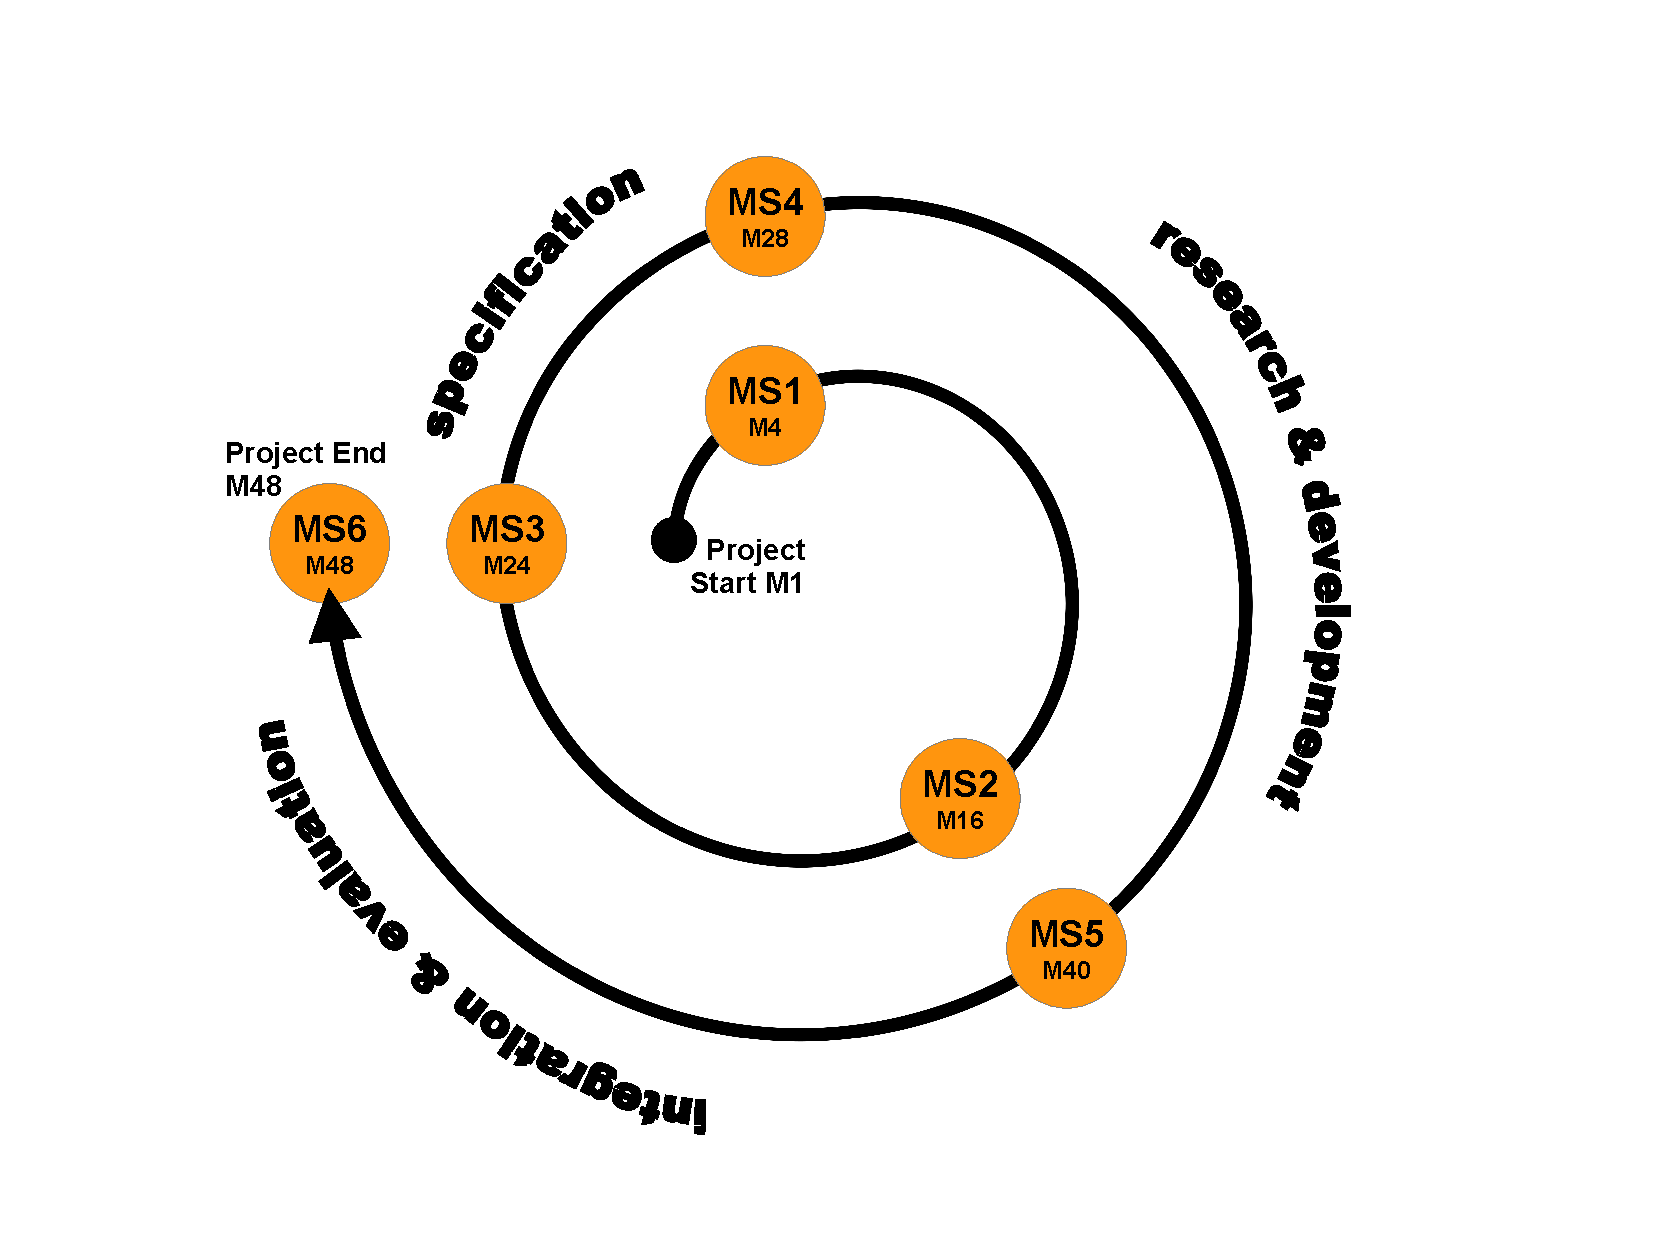
\includegraphics[width=0.6\textwidth]{pics/spiralOverview.pdf}
   \caption{Spiral life-cycle model used in \Project}
\end{wrapfigure}
   \label{fig:spiral}

This model was very successfully applied in previous EC-funded projects by members of the consortium. Using this model for our new endeavor \Project{} will allow us to test and evaluate new developments at early stages.  The spiral development model has the further advantage that it is a risk-reduction oriented model that breaks a project up into smaller projects, the cycles. This allows for improving specifications as experience is gained, and for providing feedback from trials early on in the project.  In the case of \Project, the spiral development model incorporates an intermediate trials/validation phase by the end of the first cycle, which is immediately followed by a re-specification phase (first phase of second cycle). Depending on the results of the intermediate test and validation, the Consortium will refine functional and technical specifications -- and also plan for specific actions that need to be executed in order to mitigate risks.  Within \Project{} risks are taken seriously and are specified for each work package individually. This risk analysis is continuously carried out during the whole project to react to risks as they emerge and minimize their impact on the project.

\paragraph{\textbf{Partner Interaction}}

 The consortium has been primarily assembled according to the individual members' leading expertise in the complementary domains required for successfully completing the bold aims of \Project. However, equally important for the project's success, the consortium members also spot a substantial record of successful previous collaboration (see Section~\ref{sec:consortium})-- thereby reducing interaction-related project risks substantially. To this end, and as has been proven to be successful in the past, integration efforts will commence very early in the project in alignment with the modular approach proposed above.

Although the work is separated into work packages to create efficient interfaces, as described below, all partners will closely collaborate from the onset at and across these interfaces. Meetings between the participants, as well as four consortium-wide integration and testing weeks, for which all partners meet to boost the integration of the individual components, will be carried out during the project at months M17, M24, M41 and M48. The second and fourth of these meetings will coincide with the intermediate and final project evaluation, respectively. In between physical meetings, there will be frequent exchange via telephone, email, a common repository for developments, and web-based services such as forums or status report pages. All of these will serve to boost the integration of our work, to identify problems early on and to measure the progress of the project. We are convinced that a proper joint integration is key in large-scale robotics projects with a significant degree of autonomous behavior, especially if the robots operate in challenging and complex environments as the ones addressed in this project. 

%\begin{figure}[ht]
%\centering
%\subfigure[Spiral life-cycle model used in \Project]{
%   \includegraphics[width=0.45\textwidth]{pics/spiral.jpg}
%   \label{fig:spiral}
% }
% \subfigure[Work Package Overview with key interfaces between the individual work packages.]{
%   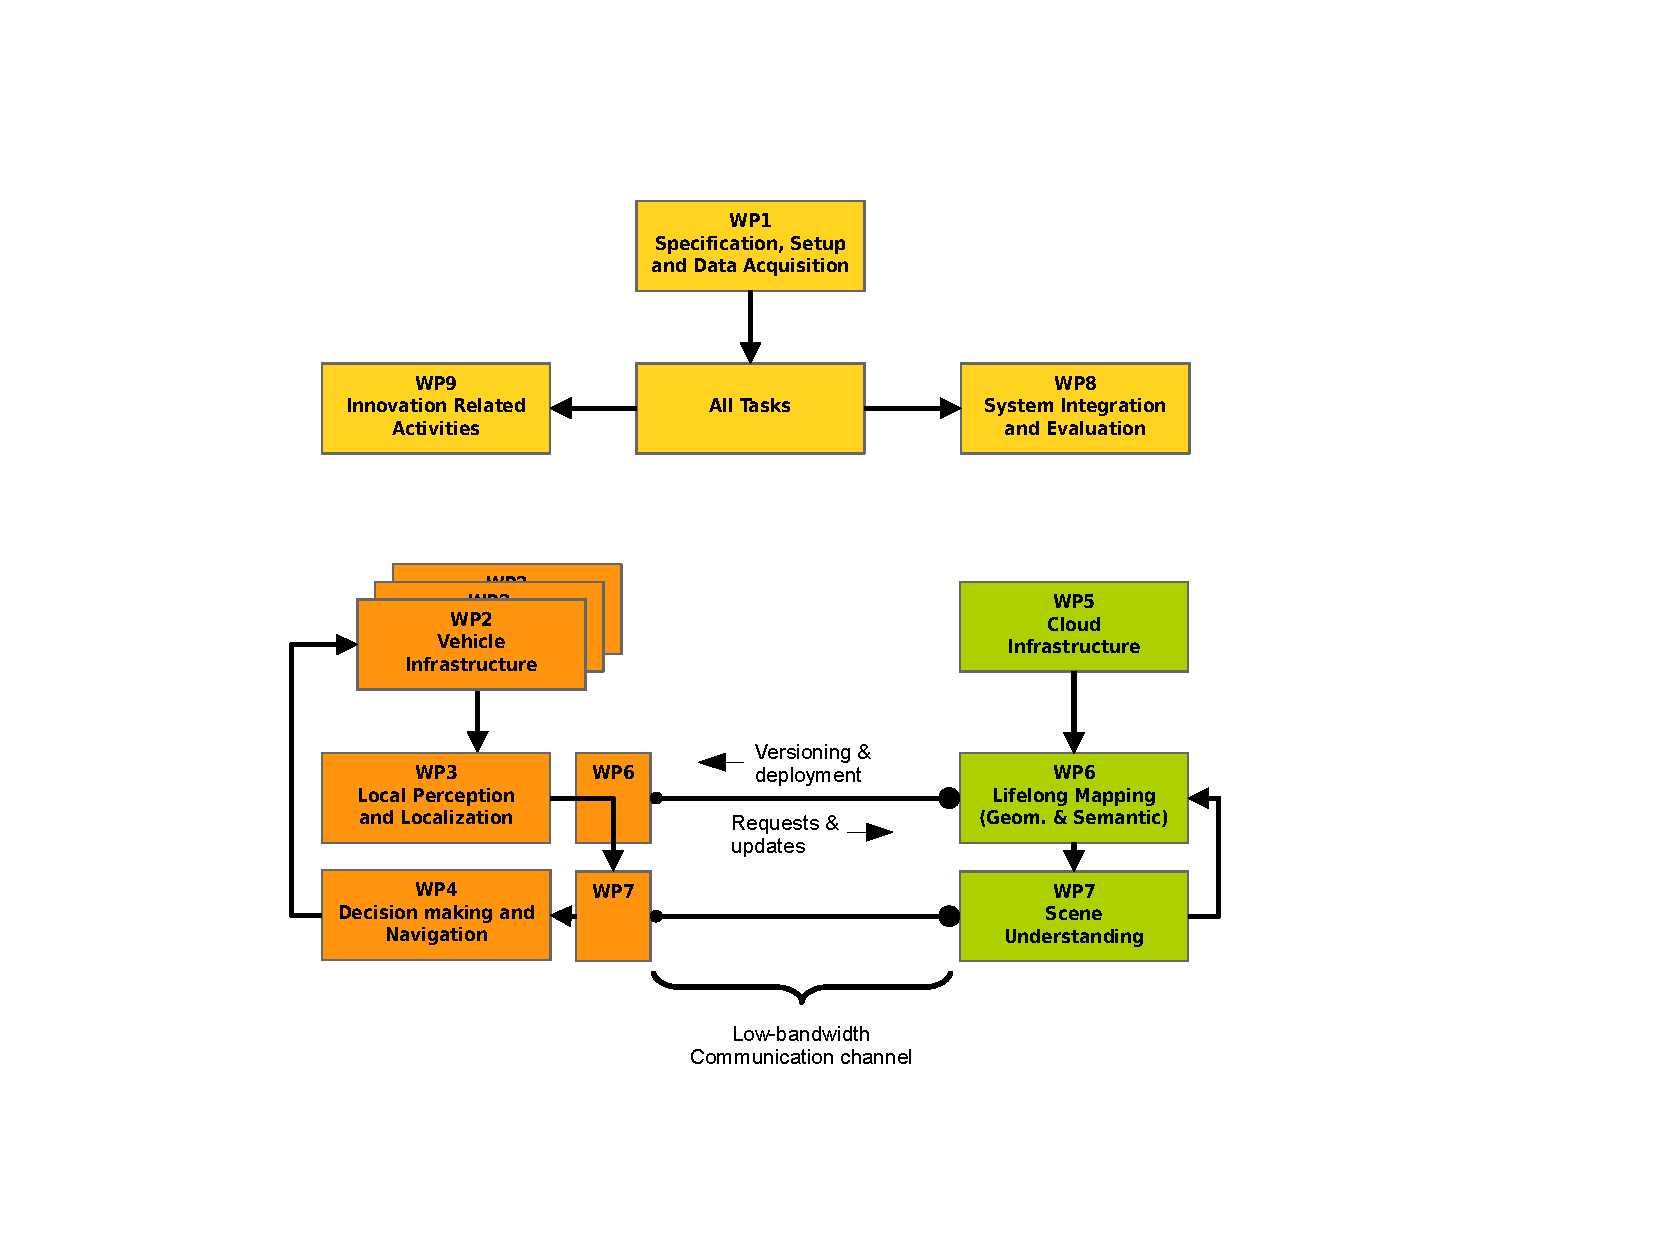
\includegraphics[width=0.45\textwidth] {pics/wpOverview.jpg}
%   \label{fig:wpOverview}
% }
%\label{fig:xxxx}
%\caption{Spiral life cycle model and associated work packages. \todo{\IBM: redo}}
%\end{figure}

\begin{figure}[ht]
  \centering
   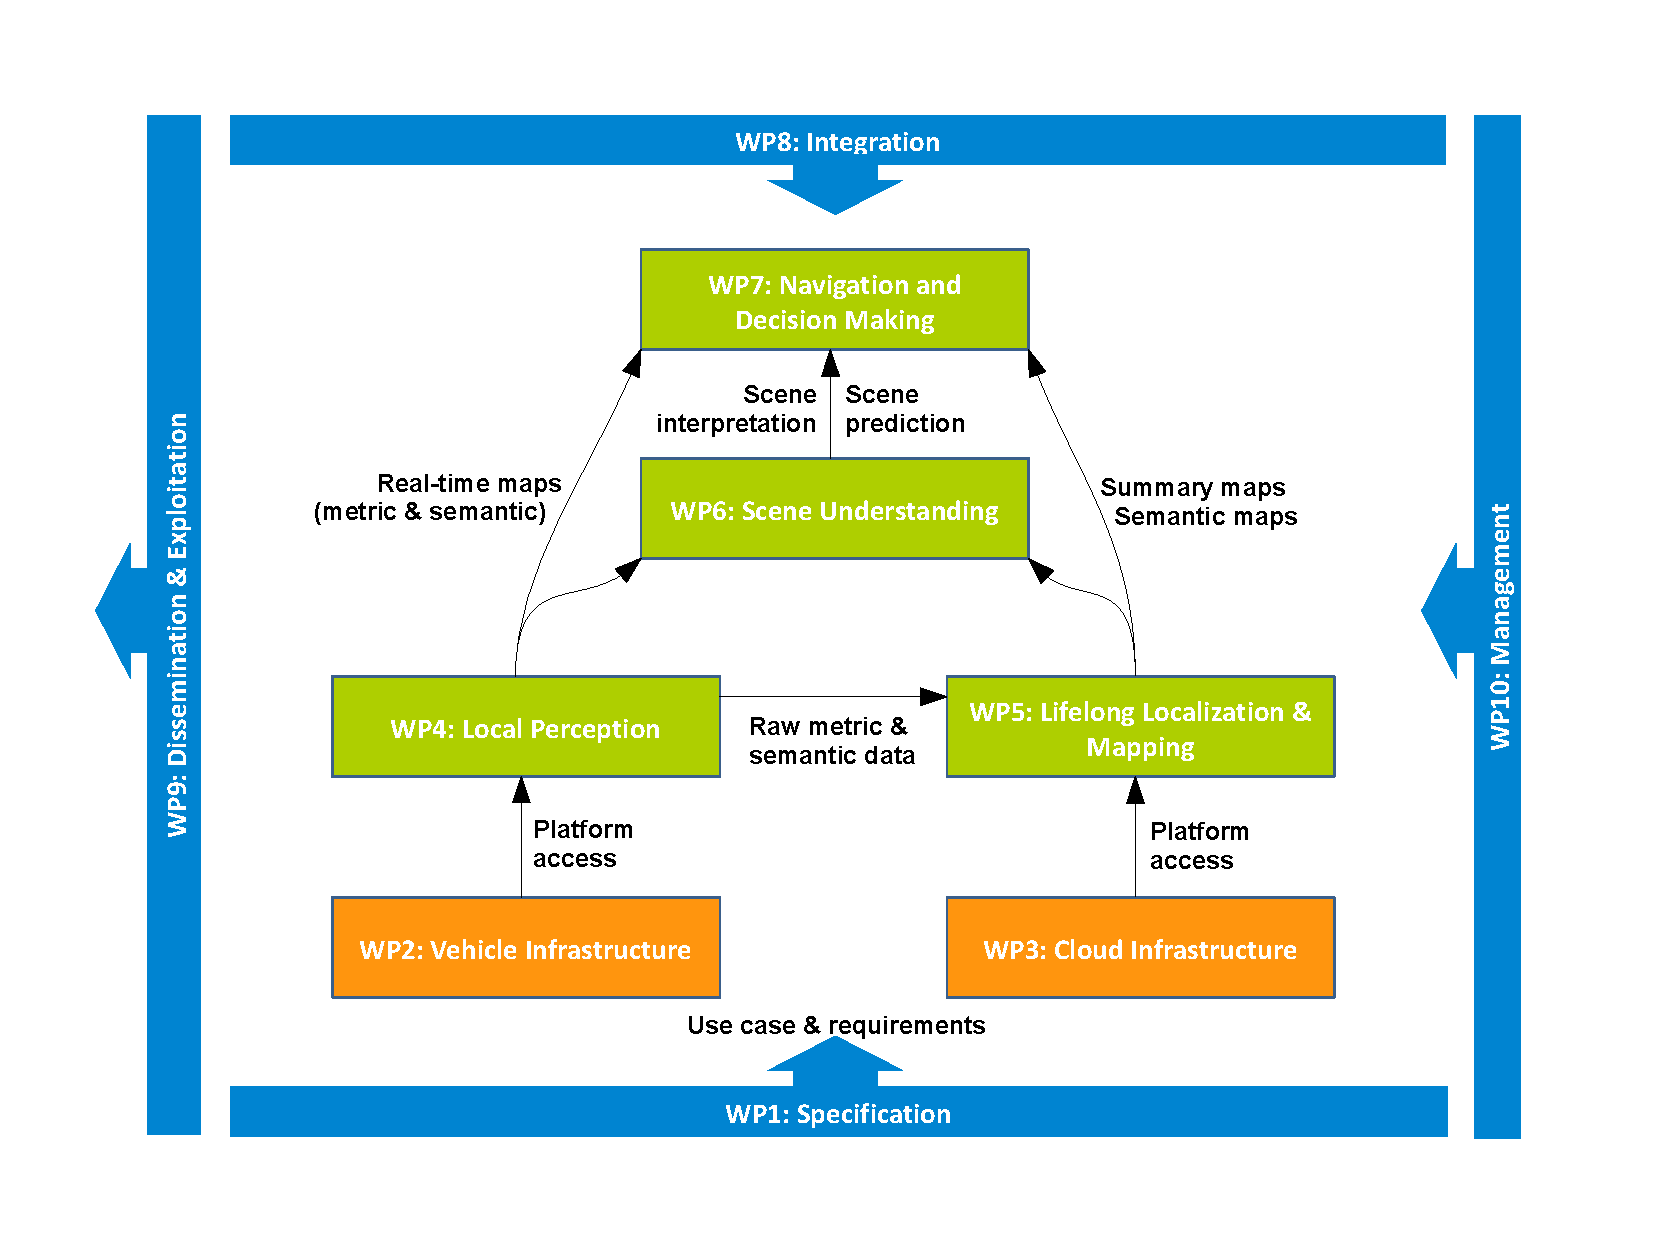
\includegraphics[width=0.8\textwidth] {pics/wpOverviewV2.pdf}
   \caption{Work Package overview with key interfaces between the individual work packages.}
   \label{fig:wpOverview}
\end{figure}



\subsubsection{Detailed Implementation Plan and Work Package Overview}
\label{sec:implementationplan}

The development \& implementation plan of \Project{} follows a logical partition of the work based on the applications addressed within the project. It separates key problems into individual work packages and entrusts their coordination to the consortium partner with the strongest expertise in that area. As a result, the work in \Project{} is  structured into the six technical work packages (WP2 -- WP7) each corresponding to a different key technical or scientific topic that will be addressed, one work package each for the Use Case \& Requirements Specification (WP1), and System Integration \& Evaluation (WP8), respectively -- in alignment with the spiral life cycle model employed. Finally, the project maintains a work package covering important innovation-related activities including dissemination and exploitation (\WPInnovation), and a work package covering aspects related to project management (\WPManagement). Table~\ref{wpleadertab} provides an overview.

\label{wpleadertab}
\begin{center}
{\small
  \begin{tabular}[h]{|c|l|l|}\hline
    {\highlightCell WP} & {\highlightCell Addressed Project Part} & {\highlightCell WP Leader} \\\hline\hline
    \WPSpecificationNo &   \WPSpecificationTitle & \CLUJ \\
    \WPVehicleNo &  \WPVehicleTitle  & \VW \\
    \WPCloudNo & \WPCloudTitle & \IBM \\
    \WPPerceptionNo & \WPPerceptionTitle & \CLUJ \\
    \WPMappingNo & \WPMappingTitle & \ETHZ \\
    \WPSceneUnderstandingNo & \WPSceneUnderstandingTitle & \PRAGUE \\
    \WPNavigationNo & \WPNavigationTitle & \VW \\
    \WPIntegrationNo & \WPIntegrationTitle & \VW \\
    \WPInnovationNo & \WPInnovationTitle & \IBM \\
    \WPManagementNo & \WPManagementTitle & \VW\\
    \hline
  \end{tabular}
}
\end{center}

Each work package is in turn split into several tasks to provide a more detailed structure including an assignment of responsibilities to the individual partners. A detailed description of the work packages, including the connection to other WPs, the personnel resources, tasks, as well as the resulting deliverables is the topic of the remainder of this section.

Before explaining the work packages and involved task in detail starting on Page~\pageref{wp1}, however, we briefly summarize the key topics addressed in the work packages and their inter-dependencies. Please also refer to  Table~\ref{tab:wpoverview} on Page~\pageref{tab:wpoverview} as a  quick reference for the tasks in the work packages and Figure~2 on Page~\pageref{fig:wpOverview} for a chart illustrating the connections between work packages. 



%%%%%%%%%%%%%%%%%%%%%%%%%%%%%%%%%%%%%%%
\paragraph{\textbf{\WPSpecification: \WPSpecificationTitle}} 
This work package targets the overall application-specific challenges of the project and together with \WPIntegration \space enables system-wide considerations within the spiral life-cycle model adopted in \Project (see Figure~\ref{fig:spiral} on Page~\pageref{fig:spiral}). In particular, end user needs and requirements are analyzed with respect to the proposed applications -- which in turn lead to a concretized application specification. Based on these requirements, the structural and functional architectures of the system and components will be specified. During the project duration two cycles of specification and re-specification are performed.


%%%%%%%%%%%%%%%%%%%%%%%%%%%%%%%%%%%%%%%
\paragraph{\textbf{\WPVehicle: \WPVehicleTitle}}
The goal of this work package is to provide fully operational automated vehicles serving the project as data collection platforms, for the test and evaluation of the  perception, localization and mapping, scene interpretation and actuation functionality developed in work packages 4--7, as well as for the demonstration of the overall applications. A fully operational platform will be made available quickly to accelerate research by refurbishing a vehicle from the V-Charge project. Specifications from \WPSpecification will be addressed completely by designing an additional vehicle within the \Project{} project -- available by the second project half. The work package covers the following aspects:
\begin{denseItemize}
\item \textbf{Vehicle buildup} including sensor system, computer system, communication system (in-vehicle as well as between vehicles) as well as HMI elements
\item \textbf{Enabling automated operation} through actuation of all relevant vehicle systems: gas, brakes, steering wheel, gearbox, parking brake, etc.
\item Design and implementation of a framework for \textbf{low-level data acquisition, processing \& communication}
\item\textbf{Calibration and data integrity validation} of the sensor system
\item Installation and integration of \textbf{reference sensors for ground-truth measurements}
\item \textbf{Vehicle maintenance and updates}
\end{denseItemize}


%%%%%%%%%%%%%%%%%%%%%%%%%%%%%%%%%%%%%%%
\paragraph{\textbf{\WPCloud: \WPCloudTitle}}
In this work package a project-wide foundational layer for cloud infrastructure is designed and implemented, allowing for the development, deployment, testing, and operation of the software developed in \Project. This infrastructure consists of a foundational hardware stack and a software stack for managing development, deployment, operation, and long-term data storage. Key activities in \WPCloud include:
\begin{denseItemize}
\item Setup of \textbf{project-wide development infrastructure}. In order to enable collaborative system development state-of-the-art tools will be installed and made accessible to all partners. These include software repository, wiki, issue tracking system, test data server.
\item \textbf{Server hardware specification and setup}. The hardware stack will consist of compute nodes, accelerators, memory, storage
  and communication infrastructure, and will be scoped based on the functional
  and application requirements derived in \WPSpecification.
\item Design of a \textbf{development and deployment tool chain} consisting of a configuration management system and a continuous integration system.
\item Setup of a \textbf{cross-device communication framework} ensuring messaging between applications in the software stacks on the vehicles
  and on the server.
\item Setup and implementation of the \textbf{bulk data storage service} consisting of an object store such as OpenStack Swift, which is ideal for storing unstructured data that can grow without bound. Data storage will be built for scale and optimized for durability, availability, and concurrency across the entire stored data set.
\end{denseItemize}

%In this work package a project-wide foundational layer for the compilation, testing, deployment and operation of project functionality as well as the storage, processing, maintenance and sharing of data across devices is implemented. The framework spans hardware and software infrastructure stacks on the cars as well as on a dedicated server. It exposes a common front-end allowing the same applications (i.e., mapping, localization and scene understanding functionality) to operate on either stack -- with the sole difference being the amount but not the type of resources (compute, memory, storage, data) available to them. Activities in \WPCloud include:
%\begin{denseItemize}
%\item \textbf{Hardware stack}. The hardware stack will be formed by distinct vehicle and server side setups of compute nodes, accelerators, and memory \& storage. The compute nodes are built around IBM POWER processors, building on the OpenPOWER ecosystem. These will be complemented by state-of-the-art commercial FPGA and GPU compute accelerators. Concerning memory, we will provision significant amounts (\todo{How much?}) of standard dynamic random-access (DRAM) memory in combination with non-volatile memory technologies (\todo{RAMDISK?}). This allows the handling and manipulation of significant chunks of the knowledge graph in memory -- thereby practically enabling the large-scale map maintenance and scene understanding applications covered in \Project{}. 
%
%\item \textbf{Software\,/\,virtualization\,/\,runtime\,/\,deployment stack}. The software stack consists of a deployment toolchain, allowing to specify entire deployment stack (OS, system libraries, databases) and dependencies (data type subscriptions, what to do if dependencies change)  in a proper language. It further provides functionality for automatic compilation and testing of committed software, as well as its deployment. \todo{The idea is that each functionality can specify its own operating system, etc. Everything is virtualized and many such instances may run on the same hardware. Communication is via message passing over TCP (e.g., via MQTT). Furthermore, we need to ensure that each of the virtual machines has access to some joint storage DBs, such as the map. The map DB and maintenance could again be specified as a virtual machine... }. \todo{A runtime scheduler will be part of each virtual machine, and will execute the programs based on scripted events and conditions}. \todo{Deployment will be specified from a separate serer instance (e.g., where the overall code will be maintained), and can be scripted such that entire stacks and stack dependencies are deployed to the server and the vehicles. Prior to deployment we will provide functionality for automated compilation, testing of code based on predefined rules (i.e., once every x duration, or once dependencies have changed). Web-based access control and commit control}. \todo{We need to deploy a yellow-zone server!!}.
%
%\item \textbf{Messaging}. Communication between vehicles and the server and, indeed, between the various virtual machines on every hardware stack will be implemented based on the publish-subscribe principle. We intend to use the the open source Message Queue Telemetry Transport (MQTT) standard originally developed at IBM to this end. It features precise access control, data encryption, small overhead communication important for wireless operation, and various forms of Quality of Service (QoS)  settings.
%
%\item \textbf{Data representation \& curation}. It is extremely important that data is represented consistently over the entire project, that it is efficiently accessible by all technical functionality, and that it is curated between the vehicles and the server. Tasks include knowledge representation and storage. This will be done as a knowledge graph, unifying metric and semantic maps of WPxx and semantic extractions of WP3, and providing a single interface for scene interpretation (WP7). Particular focus will be laid on the propoer data structures and storage location for each of the data sources. Other tasks include data curation, hence the adding, deleting, merging -> essentially versioning) consistent representation across devices, dependency handling. We will begin with a centralized approach orchestrated from the server, and will then also consider more decentralized options.
%\end{denseItemize}


%%%%%%%%%%%%%%%%%%%%%%%%%%%%%%%%%%%%%%%
\paragraph{\textbf{\WPPerception: \WPPerceptionTitle}}
This work package provides the vehicle-side online sensing functionality required for automated driving in low-speed urban environments. The work package covers the following primary aspects:
\begin{denseItemize}
\item \textbf{Specification and design of on-board sensing}
\item \textbf{On-board 360\degree \space multi-sensorial perception} based on a set of well selected sensors including laser scanners, radars, large field of view cameras, and stereo cameras disposed in a configuration offering good coverage, redundancy and good measurement accuracy.

\item \textbf{Spatio-temporal and appearance based low-level representation} The low level representation will integrate 3D position, 3D motion and intensity or color components. This will benefit from the fusion of low-level information coming from multi-sensors.

\item \textbf{Refinement of detection, tracking, and classification capabilities and environment sensorial representation}. The intention is to use a spatio-temporal and appearance based low level representation for each pixel, feature or object consisting of 3D position, 3D motion and intensity or color components. This approach will lead to a better detection or clustering of the object or object parts, to a better tracking and classification. Word Channel and Deep Learning methods will be investigated for improving the classification results.
%\item Generation of an environmental model suitable for automated navigation. Compact representation methods will be investigated and developed for environment representation starting from the classified elevation map, stixel representation and 3D voxel representation.
\end{denseItemize}


%%%%%%%%%%%%%%%%%%%%%%%%%%%%%%%%%%%%%%%
\paragraph{\textbf{\WPMapping: \WPMappingTitle}}
This work package develops metric accurate localization and lifelong mapping functionality across vehicles and the server backend. To this end raw sensor as well as semantic data recorded and made available in \WPPerception is collected in a cloud-based mapping backend, where relevant information is extracted and condensed into a compact map representation that can  efficiently be distributed back to the vehicles for localization purposes. The WP can be divided into three key areas:
\begin{denseItemize}
\item \textbf{Online Localization and Mapping} This task employs real-time online localization algorithms on the vehicles. Locally relevant map segments are requested from the mapping backend. Local sensor data is then matched against the map to be able to estimate the vehicle's pose in the map. To guarantee uninterrupted localization availability under all conditions, novel ways to deal with lighting, weather and seasonal change have to be investigated. Research in this area involves striving for performance wrt. metric accuracy, speed and data transmission rates, as well as increasing robustness to appearance change and developing new and efficient ways to feed sensor data back to the mapping backend.
\item \textbf{Map Maintenance and Summarization}. The mapping backend collects sensor data from various agents over long-term operations. Algorithms to assess data accuracy and trustworthiness, to handle structural change as well as encode different appearances are necessary to allow long-term localization in changing environments. It is the scope of this task to collect, assess, register and filter incoming data and to produce compact generic representations ('summary-maps') encoding the most useful information for localization independent of the current environmental conditions. These summary-maps can then be fed back on request to the agents for efficient localization purposes.
\item \textbf{Semantic Information Integration}. The map described above will serve as a backbone for all kinds of higher level semantic information to be represented in. While collecting, classifying and representing this semantic information is done within the scope of \WPPerception and \WPSceneUnderstanding, the map backend enables integration, managing and versioning of the semantic information.
\end{denseItemize}


%The goal of this WP is to provide metrically accurate localization at all times. For this, a map of the agent's environment is recorded, managed and curated.
%The map contains enough information to allow metrically accurate localization across all possible environments, weather and lighting conditions, including night-time.
%Raw sensor data from various agents is collected in a cloud-based mapping backend, where relevant information is extracted and condensed into a compact map representation that can  efficiently be distributed back to the agents for localization purposes. This forms a closed-loop cycle between a fleet of agents and the mapping backend infrastructure.
%In this way, the map is continuously updated and maintained respecting both appearance and structural change on short-term to long-term time scales.
%It further  provides geometrically consistent coordinate frames in which higher level semantic information can be registered.
%\begin{figure}[H]
%\begin{center}
%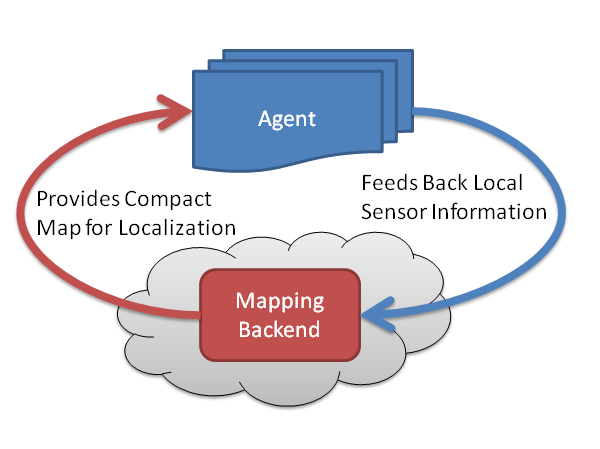
\includegraphics[width=0.5\textwidth]{pics/localization_feedback_loop.png}
%\caption{Feedback-Loop Between Multi-Agent Localization and the Cloud-Based Mapping Backend.}
%\label{fig:pert}
%\end{center}
%\end{figure}
%
%The WP can be divided into four main sub-tasks as follows:
%\begin{denseItemize}
%\item \textbf{Online Localization} This task employs real-time online localization algorithms on the agents. Locally relevant map segments are requested form the mapping backend. Local sensor data is then matched against the map to be able to estimate the agent's pose in the map. Research in this area involves striving for performance wrt. metric accuracy, speed and data transmission rates, as well as developing new and efficient ways to feed sensor data back to the mapping backend.
%
%\item \textbf{Apperance-Based Localization and Mapping}. Accurate and uninterrupted localization around the clock, across seasons and varying weather conditions forms a key requirement for all tasks involved in this project. In order to achieve this goal, identifying the current environmental condition and using this information to infer what sensor data is likely to appear in the imminent future is key and the scope of this task. It shall also allow formulating specific appearance related requests to the mapping backend depending on the current environment condition the agent is perceiving.
%
%\item \textbf{Map Maintenance and Summarization}. The mapping backend collects sensor data from various agents over long-term operations. Algorithms to assess data accuracy and trustworthiness, to handle structural change as well as encode different appearances are necessary to allow long-term localization in changing environments. It is the scope of this task to collect, assess, register and filter incoming data and to produce compact generic representations ('summary-maps') encoding the most useful information for localization independent of the current environmental conditions. These summary-maps can then be fed back on request to the agents for efficient localization purposes.
%
%\item \textbf{Semantic Information Integration}. The map described above will serve as a backbone for all kinds of higher level semantic information to be represented in. While collecting, classifying and representing this semantic information is done within the scope of WP3 and WP7, the map backend developed in WP6 must allow integrating and managing the semantic information in the mapping backend respectively. This task aims at developing a smooth framework and process for semantic data to be integrated into the mapping backend.
%\end{denseItemize}


%%%%%%%%%%%%%%%%%%%%%%%%%%%%%%%%%%%%%%%
\paragraph{\textbf{\WPSceneUnderstanding: \WPSceneUnderstandingTitle}}
Beside local perception it is important to provide the navigation module of \WPNavigation with a high level assessment of the environment, in order to assist it in selecting the proper driving behavior. This work package targets all aspects contributing to understanding the local scene in the surroundings of the car, including driving mode and behavior of other roads occupants. It will hence explore and develop techniques
\begin{denseItemize}
\item to \textbf{represent the environment in scenarios},
\item to fuse information from various \Project{} sensor sources and derivatives thereof (including digital maps, online raw sensor perception, road users' behavior perception, current location, and further contextual information) to create a \textbf{high level scenario description and interpretation}. Examples of such a high-level interpretation include: other car willing to overtake; other car willing to exit the lane; traffic jam ahead; road work; and entering pedestrian area,
%\item for \textbf{context based road users' behavior analysis}. We will extend the dynamic object tracking techniques developed in \WPPerception by complementing them with visual perception information and high level reasoning, to create a profile of each road user surrounding the ego vehicle.
\item for object motion prediction or \textbf{scene prediction}, which is guided by the high-level scenario/behavior information,
\item for \textbf{self-assessment}. Data from Work Packages 4-6 will be analyzed to identify potential data integrity issues or infer context-dependent system limitations.
\end{denseItemize}


%%%%%%%%%%%%%%%%%%%%%%%%%%%%%%%%%%%%%%%
\paragraph{\textbf{\WPNavigation: \WPNavigationTitle}}
In this work package decision making and navigational abilities necessary for automated operation in urban areas are adapted from previous projects of the consortium members and further developed. This work package relies on information from the online local perception, scene understanding, as well as from offline metric and semantic mapping. The activities within this task range from route and tactical planning, to maneuver and trajectory planning, to trajectory control. The decision making and navigation stack will take into account constraints arising from traffic rules, collision risks, time budget for reaching the target destination, etc. Attention will be also devoted the question of map verification and fall back strategies in case the map turns out to be outdated/erroneous.


%%%%%%%%%%%%%%%%%%%%%%%%%%%%%%%%%%%%%%%
\paragraph{\textbf{\WPIntegration: \WPIntegrationTitle}}

The individual components of \Project{} -- grouped into work packages -- can be developed and evaluated individually to some extent only.  As Figure~\ref{fig:wpOverview} on Page~\pageref{fig:wpOverview} illustrates, information exchange and thus interdependency between the tasks and WPs is substantial. Integration and evaluation at the system level, with a strong focus on the proposed applications, thus becomes critical.

To this end, \WPIntegration will be responsible for the integration and testing of the individual modules, as well as system-wide testing and validation with a special emphasis towards the proposed applications. This includes the organization of the integration and testing weeks and the smooth integration of the technologies developed in this project. Thus, all work packages will strongly interact with \WPIntegration. Activities in \WPIntegration include:
\begin{denseItemize}
%mru: moved to cloud infrastructure WP
%\item \textbf{Development Repository}. All partners will contribute software modules for the integrated system. The versions of all software modules will be handled using a central development repository with access to all partners.
\item \textbf{Integration Plan}. The integration plan will specify which components have to provide certain functionality to allow for a successful integration. It will furthermore contain a detailed time line for the integration and thus serves as a manual for the integration weeks.
\item \textbf{Integration tools and processes}. In order to make the integration and test efficient and effective a set of tools and processes will be installed or developed, including checklists, and developer guidelines.
\item \textbf{System Integration and Testing Weeks}. We will have four integration and testing weeks throughout the project life time and the integration task will start early on so that a first integrated working system becomes available early in the project life-cycle. The four integration and testing weeks will be the key concept to ensure a smooth integration of all the individual modules to a working subsystem. They will bring together the researchers, help to identify problems, and boost the overall development process.
\item \textbf{Evaluation}. A proper evaluation is essential to measure the capabilities of the system, scientific advancement, and  the success of the overall project. This work package thus on one hand addresses the evaluation of the individual components; the measures for success, specified in the individual work packages, will serve as the basis for the evaluation. On the other hand \WPIntegration will measure the performance of the overall integrated system as specified by the application scenarios. Finally scientific progress will be evaluated by the quality and quantity of papers published in journals and relevant conferences. 
\end{denseItemize}


%%%%%%%%%%%%%%%%%%%%%%%%%%%%%%%%%%%%%%%
\paragraph{\textbf{\WPInnovation:  \WPInnovationTitle}}
This work package covers the following aspects:
\begin{denseItemize}
\item \textbf{Dissemination activities}: ensuring the proper dissemination of the \Project{} project and promoting awareness of results in the general, business and scientific community at large. This is envisioned to be in the form of documents, brochures, Web-publications, workshops, articles, papers for journals and conferences or other publicity work. More details on planned dissemination activities can be found on Page~\pageref{sec:diss}.
\item \textbf{Exploitation plan} ensuring the proper exploitation of the \Project{} results. This includes activities such as an address database of related stakeholders, potential customers, interested individuals and companies, and the identification and pursuing of exploitable results. More information on exploitation activities can be found on Page~\pageref{sec:expl}.
\item \textbf{Management of Knowledge including IPR handling}. This will include an internal collaboration environment in addition to the public website, and data management ensuring that data produced by the project is available for further research -- while respecting the data policies of the consortium members. In addition this aspect ensures IPRs are properly handled and patents are filed where and when necessary. More detail on the planned management of knowledge and IPR handling can be found on Page~\pageref{sec:iprhandling}.
\end{denseItemize}


%%%%%%%%%%%%%%%%%%%%%%%%%%%%%%%%%%%%%%%
\paragraph{\textbf{\WPManagement: \WPManagementTitle}}
The \Project{} project management structure is characterized by the following formal roles: (i) Project Coordinator and Steering Committee; and (ii) Work package leaders. In terms of formal process, the work package leaders will be responsible for the planning, scientific management and progress of their work package and will have to report the progress to the project coordination team consisting of the Project Coordinator \Coordinator{}. The work package leaders' responsibility is further to identify and highlight problems as early as possible. This approach ensures a task-driven scientific management while maintaining effective overall control by the coordination team.  For the day-to-day work on the project, virtual project teams are formed according to the involved participants in the individual tasks. The Steering Committee -- formed by representative from each partner -- serves as the main forum for decisions and the responsible instance to resolve disputes. Decisions will require majority and will be binding. Besides the formal channels described above, communication will also be performed on a non-periodic basis for the exchange of unstructured information as well as the rapid clarification of details, etc. In this way, the consortium will effectively track the progress of project activities while, at the same time, it will keep the administration overhead at a low level. A more detailed account of the \Project{} project management structure is provided in Section~\ref{sec:management} starting on Page~\pageref{sec:management}.



% !TEX root = ../proposal.tex

 \renewcommand{\arraystretch}{0.75}
\begin{table}[t]
\begin{center}
{  \fontsize{9}{11pt}\selectfont
\begin{tabular}{|l|p{7.9cm}|p{1.35cm}|p{0.8cm}|p{0.9cm}|p{0.9cm}|}
\hline
\highlightCell WP & \highlightCell Work package title &  \highlightCell Leader (no) & \highlightCell PMs & \highlightCell Start month & \highlightCell End month
\\ \hline\hline

\WPSpecification &
\textbf{Req., System \& Component Spec. and Arch.}\newline
 {\scriptsize
 Task~\WPSpecificationNo.1: End-user needs and requirements analysis
 \newline
 Task~\WPSpecificationNo.2: Application analysis and requirement specification
 \newline
 Task~\WPSpecificationNo.3: Definition and specification of system architecture
 \newline
 Task~\WPSpecificationNo.4: System hardware and software components specification
 }
 & \CLUJ\newline(\CLUJNo)  &
\WPSpecificationSUM
& M1 & M28
\\ \hline

%-------------------------------

\WPVehicle &
{\bf \WPVehicleTitle}\newline
 {\scriptsize
 Task~\WPVehicleNo.1: Vehicle platform setup
 \newline
 Task~\WPVehicleNo.2: Drive by wire functionality
 \newline
 Task~\WPVehicleNo.3: Low-level data acq., proc. \& comm. framework
 \newline
 Task~\WPVehicleNo.4: High level system debugging \& maintenance framework
 \newline
 Task~\WPVehicleNo.5: Calibration \& data integrity validation of the sensor system
 \newline
 Task~\WPVehicleNo.6: Reference sensor integration
 \newline
 Task~\WPVehicleNo.7: Vehicle maintenance and update
 }
 & \VW\newline(\VWNo)  &
\WPVehicleSUM
& M1 & M28
\\ \hline

%-------------------------------

\WPCloud &
{\bf \WPCloudTitle}\newline
 {\scriptsize
 Task~\WPCloudNo.1: Setup of project-wide development infrastructure
 \newline
 Task~\WPCloudNo.2: Setup of hardware stack
 \newline
 Task~\WPCloudNo.3: Design and impl. of the devel. and deployment tool chain
 \newline
 Task~\WPCloudNo.4: Setup and implementation of a communication framework
\newline
 Task~\WPCloudNo.5: Setup and implementation of the bulk data storage service
 \newline
% Task~\WPCloudNo.6: Setup and impl. of a server-side monitoring service
 }
 & \IBM\newline(\IBMNo)  &
\WPCloudSUM
& M1 & M32
\\ \hline

%-------------------------------

\WPPerception &
{\bf \WPPerceptionTitle}\newline
 {\scriptsize
 Task~\WPPerceptionNo.1: Specification and design of on-board sensing
% \newline
% Task~\WPPerceptionNo.2: System-wide data acquisition
 \newline
 Task~\WPPerceptionNo.2: Spatio-temporal and appearance based low level rep.
 \newline
 Task~\WPPerceptionNo.3: Perception adaptation to adverse visibility conditions
\newline
 Task~\WPPerceptionNo.4: Road infrastructure perception
 \newline
 Task~\WPPerceptionNo.5: Real-time 3D terrain perception
 \newline
 Task~\WPPerceptionNo.6: Road users perception \& signaling detection
 \newline
 Task~\WPPerceptionNo.7: Sensor fusion based perception refinement
 }
 & \CLUJ\newline(\CLUJNo)  &
\WPPerceptionSUM
& M1 & M42
\\ \hline

%-------------------------------

\WPMapping &
{\bf \WPMappingTitle}\newline
 {\scriptsize
 Task~\WPMappingNo.1: Mapping frontend
 \newline
 Task~\WPMappingNo.2: Internal map representation
 \newline
 Task~\WPMappingNo.3: Internal map storage
 \newline
 Task~\WPMappingNo.4: Highly accurate metric localization
\newline
 Task~\WPMappingNo.5: Classification and aggregation of semantic data
 \newline
 Task~\WPMappingNo.6: Map management and summarization
 \newline
 %Task~\WPMappingNo.7: Evaluation of the lifelong loc. \& mapping performance
 }
 & \ETHZ\newline(\ETHZNo)  &
\WPMappingSUM
& M1 & M42
\\ \hline

%-------------------------------

\WPSceneUnderstanding &
{\bf \WPSceneUnderstandingTitle}\newline
 {\scriptsize
 Task~\WPSceneUnderstandingNo.1: Long-term semantic scene understanding
 \newline
 Task~\WPSceneUnderstandingNo.2: Scenario based scene understanding
 \newline
 Task~\WPSceneUnderstandingNo.3: Scene prediction
 \newline
 Task~\WPSceneUnderstandingNo.4: Self-assessment
 }
 & \PRAGUE\newline(\PRAGUENo)  &
\WPSceneUnderstandingSUM
& M3 & M44
\\ \hline

%-------------------------------

\WPNavigation &
{\bf \WPNavigationTitle}\newline
 {\scriptsize
 Task~\WPNavigationNo.1: Route planning
 \newline
 Task~\WPNavigationNo.2: Tactical planning
 \newline
 Task~\WPNavigationNo.3: Trajectory planning
 \newline
 Task~\WPNavigationNo.4: Trajectory control
 \newline
 Task~\WPNavigationNo.5: Mission Executive
 }
 & \VW\newline(\VWNo)  &
\WPNavigationSUM
& M3 & M46
\\ \hline

%-------------------------------

\WPIntegration &
{\bf \WPIntegrationTitle}\newline
 {\scriptsize
 Task~\WPIntegrationNo.1: Integration Plan
 \newline
 Task~\WPIntegrationNo.2: System-wide data acquisition
 \newline
 Task~\WPIntegrationNo.3: Integration and test tools and processes
 \newline
 Task~\WPIntegrationNo.4: System integration
 \newline
 Task~\WPIntegrationNo.5: System evaluation and validation
  }
 & \VW\newline(\VWNo)  &
\WPIntegrationSUM
& M2 & M48
\\ \hline

%-------------------------------

\WPInnovation &
{\bf \WPInnovationTitle}\newline
 {\scriptsize
 Task~\WPInnovationNo.1: Management of knowledge
 \newline
 Task~\WPInnovationNo.2: Dissemination
 \newline
 Task~\WPInnovationNo.3: Exploitation
  }
 & \IBM\newline(\IBMNo)  &
\WPInnovationSUM
& M1 & M48
\\ \hline

%-------------------------------

\WPManagement &
{\bf \WPManagementTitle}\newline
 {\scriptsize
 Task~\WPManagementNo.1: Project management
 \newline
 Task~\WPManagementNo.2: Project status monitoring
  }
 &  \COORD \newline (\COORDNo) &
\WPManagementSUM
 & M1 & M48
\\ \hline\hline
-- & TOTAL &   -- &
\PMSUM
& --  & --
\\ \hline
\end{tabular}
}
\caption{Work package and task overview. }
   \label{tab:wpoverview}
\end{center}
\end{table}

Table~\ref{tab:wpoverview} on Page~\pageref{tab:wpoverview} provides an {\bf overview over the work packages} by listing the tasks addressed in
the individual work packages.

 \renewcommand{\arraystretch}{1.0}

%------------------------------------------------------------------

\begin{table}[t]
  \centering
  {  \fontsize{9}{11pt}\selectfont
\begin{tabular}{|l|p{7.6cm}|p{0.9cm}|p{1.6cm}|p{0.9cm}|p{0.7cm}|p{1.5cm}|}
\hline
\highlightCell No. & \highlightCell Deliverable name & \highlightCell WP &  \highlightCell Resp. partner & \highlightCell Type & \highlightCell Diss. level & \highlightCell Del. Date
\\ \hline\hline
D1.1 & Initial version of requirements definition, system architecture and component specification & WP1 & \CLUJ & R & PU & M4 \\\hline
D1.2 & Final version of requirements definition, system architecture and component specification & WP1 & \CLUJ & R & PU & M28 \\\hline\hline

%----------------------------------

D2.1 & First vehicle platform available & WP2 & \VW & R & PU & M8 \\\hline
D2.2 & First vehicle platform fully operational & WP2 & \VW & R & PU & M12 \\\hline
D2.3 & Second vehicle platform available & WP2 & \VW & R & PU & M24 \\\hline
D2.4 & Second vehicle platform fully functional & WP2 & \VW & R & PU & M28 \\\hline\hline

%----------------------------------

D3.1 & Development infrastructure & WP3 & \IBM & R & PU & M1 \\\hline
D3.2 & Hardware stack  & WP3 & \IBM & R & PU & M4(i), M28 \\\hline
D3.3 & Development and deployment tool chain & WP3 & \IBM & R & PU & M8 \\\hline
D3.4 & Communication framework  & WP3 & \IBM & R & PU & M12 \\\hline
D3.5 & Bulk data storage service  & WP3 & \IBM & R & PU & M16 \\\hline\hline
%----------------------------------

D4.1 & Specification and design of on-board sensing & WP4 & \CLUJ & R & PU & M8(i), M28 \\\hline
D4.2 & Low-level perception functions & WP4 & \CLUJ & R & PU & M18(i), M32 \\\hline
D4.3 & Higher-level perception functions  & WP4 & \CLUJ, \PRAGUE, \VW & R & PU & M18(i), M42 \\\hline\hline

%----------------------------------

D5.1 & Specification of the map frontend and storage concept & WP5 & \ETHZ & R & PU & M4 \\\hline
D5.2 & First development and integration cycle of lifelong mapping & WP5 & \ETHZ & R & PU & M18 \\\hline
D5.3 & Second development and integration cycle of lifelong mapping & WP5 & \IBM & R & PU & M42 \\\hline\hline
%D5.5 & Evaluation of the lifelong mapping performance & WP5 & \ETHZ & R & PU & M48 \\\hline\hline

%----------------------------------

D6.1 & Software specification and architecture for scene understanding & WP6 & \PRAGUE & R & PU & M6 \\\hline
D6.2 & First development and integration cycle of scene understanding  & WP6 & \PRAGUE & R & PU & M20 \\\hline
D6.3 & Second development and integration cycle of scene understanding  & WP6 & \PRAGUE & R & PU & M44 \\\hline\hline

%----------------------------------

D7.1 & Software specification and architecture for the decision making and navigation & WP7 & \VW & R & PU & M6 \\\hline
D7.2 & First development and integration cycle of decision making and navigation & WP7 & \VW & R & PU & M22 \\\hline
D7.3 & Second development and integration cycle of decision making and navigation & WP7 & \VW & R & PU & M46 \\\hline\hline

%----------------------------------

D8.1 & Integration plan for first development cycle & WP8 & \VW & R & INT & M12 \\\hline
D8.2 & Initial component and system data sets & WP8 & \VW & R & INT & M14 \\\hline
D8.3 & Integration and test tools and processes & WP8 & \VW & R & PU & M16 \\\hline
D8.4 & Evaluation report on integration process and results of first development cycle & WP8 & \VW & R & PU & M24 \\\hline
D8.5 & Integration plan for second development cycle & WP8 & \VW & R & INT & M30 \\\hline
D8.6 & Evaluation report on integration process and results of second development cycle & WP8 & \VW & R & PU & M48 \\\hline\hline

%----------------------------------

D9.1 & Project Web-page  & WP9 & \ETHZ  & DEC & PU & M2 \\\hline
D9.2 & Data management plan & WP9 & \ETHZ & R & PU & M4 \\\hline
D9.3 & Brochure, newsletter & WP9 & \PRAGUE & DEC & PU & M16 \\\hline
D9.4 & Press video & WP9 &  \IBM &  DEC & PU & M27 \\\hline
D9.5 & Exploitation plan & WP9 & \IBM & R & INT & M18(i), M40 \\\hline
D9.6 & Dissemination report & WP9 & \PRAGUE  & R & PU & M21(i), M45 \\\hline
D9.7 & Final demonstration & WP9 & \VW & DEC & PU & M24(i), M48 \\\hline


\end{tabular}
[R] Report, [DEC] press \& media action, [PU] Public, [INT] Internal, (i) intermediate version
}
  \caption{List of Deliverables}
  \label{tab:deliverables}
\end{table}


%---------------------------------------------------------------


\begin{figure}
\begin{center}
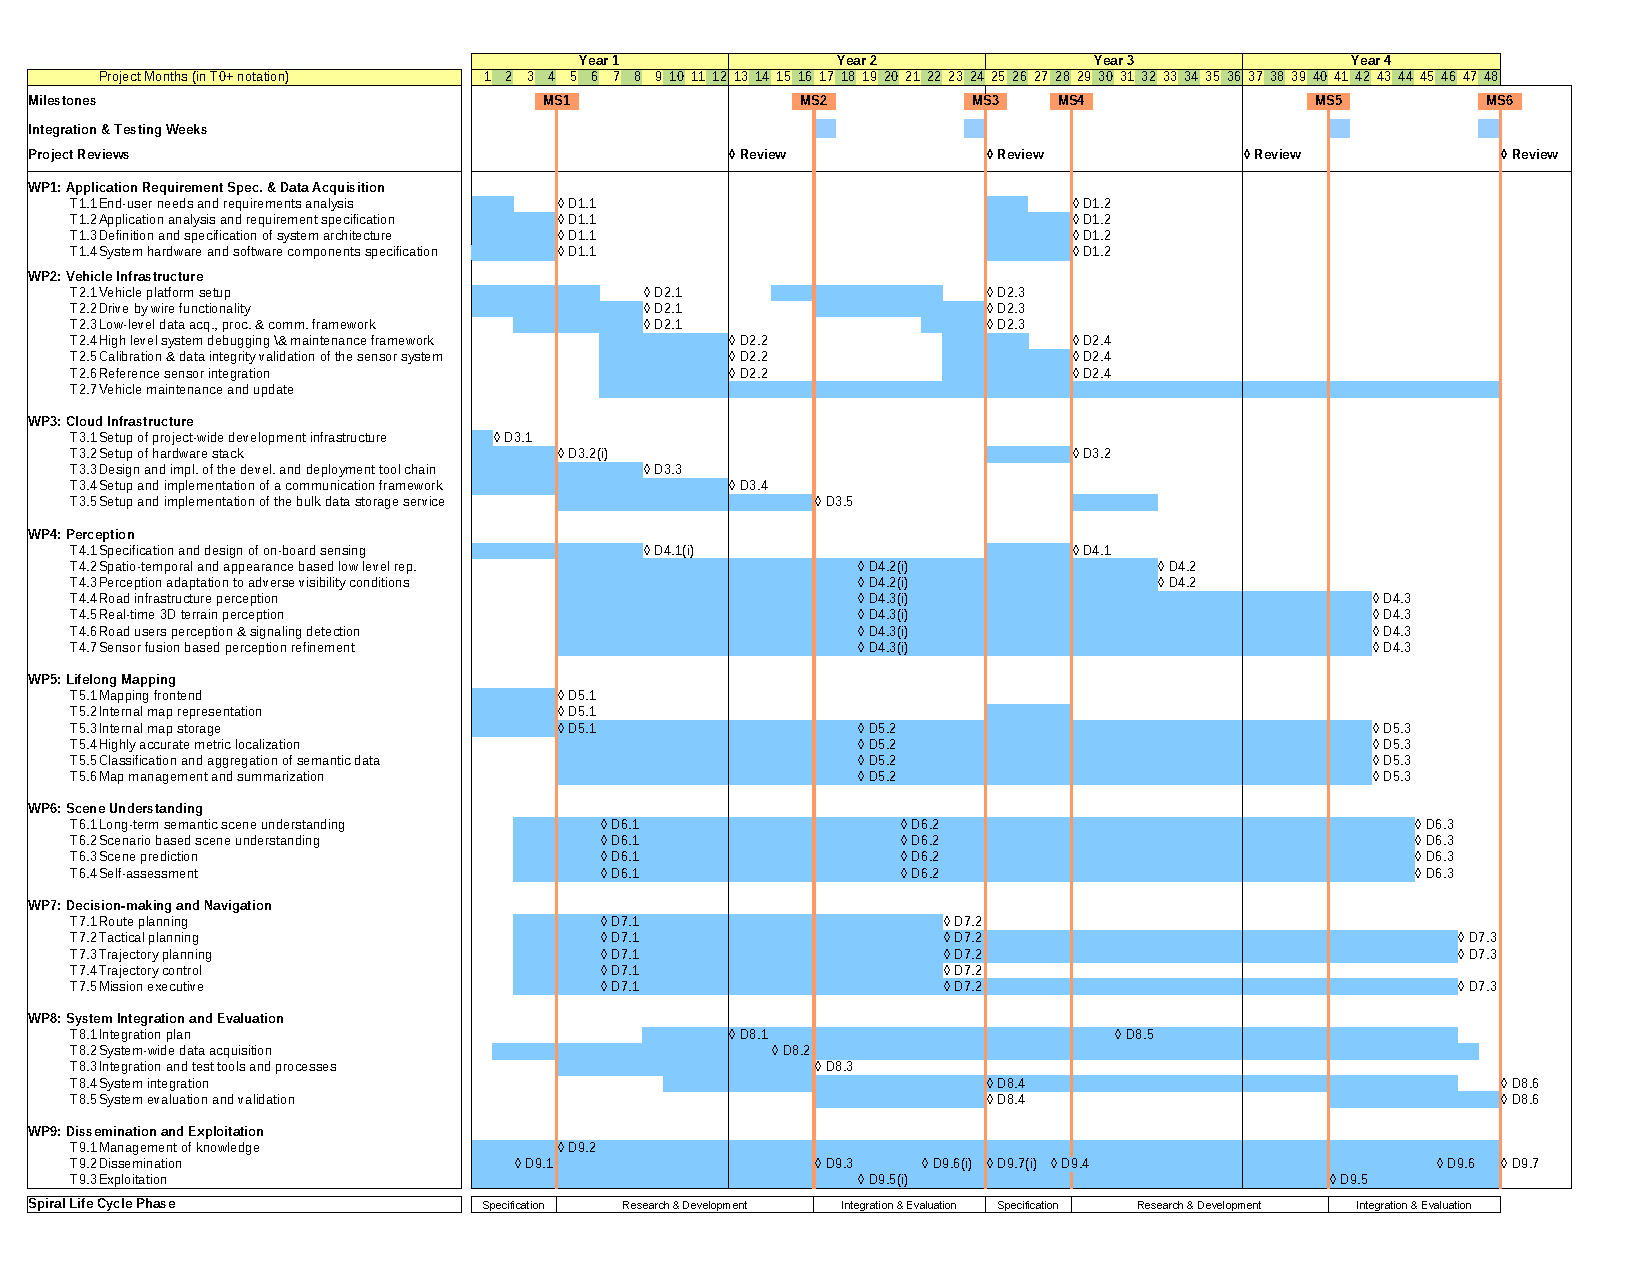
\includegraphics[angle=90,height=0.95\textheight]{pics/gantt}
\caption{Gantt chart over the whole period of the project illustrating the tasks in the work packages as well as  the Milestones and Deliverables.}
\label{fig:gantt}
\end{center}
\end{figure}



% !TEX root = ../proposal.tex

\subsubsection{Milestones}
\label{sec:milestones}

To allow for monitoring of the project as a whole, project milestones have been defined.  These events will be used to assess the current state of the work, to verify whether the necessary results have been achieved and to synchronize the activities of the consortium. Concretely, the \textbf{six milestones} mark the control points detailed in Table~\ref{tab:milestones} on Page~\pageref{tab:milestones}.  The time lines for the individual milestones (including deliverables) are presented in the Gantt chart in Figure~\ref{fig:gantt} on Page~\pageref{fig:gantt}.


%% --  --  --  --  --  --  --  --  --  --  --  --  --  --  --  --  --  --  --  --  --  -- 
\begin{table}[h!]
{\small
\begin{tabular}{|p{0.8cm}|p{11.5cm}|p{1cm}|p{1.5cm}|}
%\begin{longtable}{|p{0.9cm}|p{8cm}|p{1cm}|p{1.3cm}|p{1.7cm}|}
\hline
\highlightCell { No. } &
\highlightCell {\bf Milestone description and means of verification} &
\highlightCell {\bf Del.\newline date} &
\highlightCell {\bf Partners involved}
\\ \hline\hline

%% --  --  --  --  --  --  --  --  --  --  --  --  --  --  --  --  --  --  --  --  -- -
  \vskip0.0cm{\bf MS1}
&
  \vskip0.0cm{\bf ``Work has started, first specification completed''}

  \begin{megaDenseItemize}
  \item The consortium has met
  \item Personnel has been employed and work has been started
  \item Management structures are in place
  \item Web site is operational
  \item Development repository is in place
  \item First requirements analysis and requirements specifications complete
  \item Submitted deliverables: D1.1, D3.1, D3.2(i), D5.1, D9.1, D9.2
  \end{megaDenseItemize}
&
  \vskip0.0cm{M4}
&
  \vskip0.0cm{all}
\\ \hline\hline

%% --  --  --  --  --  --  --  --  --  --  --  --  --  --  --  --  --  --  --  --  -- -
  \vskip0.0cm{\bf MS2}
&
  \vskip0.0cm{\bf ``First development phase completed''}

  \begin{megaDenseItemize}
  \item Initial version of components has been developed and individually tested
  \item First scientific results published (at least 5 papers have been submitted to
    relevant conferences)
  \item Submitted deliverables: D2.1, D2.2, D3.3, D3.4, D3.5, D4.1(i), D6.1, D7.1, D8.1, D8.2, D8.3, D9.3
  \end{megaDenseItemize}
&
  \vskip0.0cm{M16}
&
  \vskip0.0cm{all}
\\ \hline\hline

%% --  --  --  --  --  --  --  --  --  --  --  --  --  --  --  --  --  --  --  --  -- -
  \vskip0.0cm{\bf MS3}
&
  \vskip0.0cm{\bf ``First integration and testing phase completed''}

  \begin{megaDenseItemize}
  \item The first cycle of the spiral development model has been completed
  \item First integration week has been carried out
  \item Integration and testing of initial version of components has been completed at a system level
  \item Submitted deliverables: D2.3, D4.2(i), D4.3(i), D5.2, D6.2, D7.2, D8.4, D9.5(i), D9.6(i), D9.7(i)
   
 \end{megaDenseItemize}
&
  \vskip0.0cm{M24}
&
  \vskip0.0cm{all}
\\ \hline\hline

%% --  --  --  --  --  --  --  --  --  --  --  --  --  --  --  --  --  --  --  --  -- -
  \vskip0.0cm{\bf MS4}
&
  \vskip0.0cm{\bf ``Revised specifications completed''}

  \begin{megaDenseItemize}
  \item Second integration week has been carried out
  \item At least 12 papers have been submitted to relevant conferences or journals
  \item Submitted deliverables: D1.2, D2.4, D3.2, D4.1, D9.4
   \end{megaDenseItemize}
&
  \vskip0.0cm{M28}
&
  \vskip0.0cm{all}
\\ \hline\hline

%% --  --  --  --  --  --  --  --  --  --  --  --  --  --  --  --  --  --  --  --  -- -
  \vskip0.0cm{\bf MS5}
&
  \vskip0.0cm{\bf ``All developments completed''}

  \begin{megaDenseItemize}
  \item All developments in work packages \WPVehicle--\WPNavigation{} have been completed
  \item System integration in good progress
  \item Evaluations of individual components have been conducted
  \item Submitted deliverables: D4.2, D8.5, D9.5
  \end{megaDenseItemize}
&
  \vskip0.0cm{M40}
&
  \vskip0.0cm{all}
\\ \hline\hline

%% --  --  --  --  --  --  --  --  --  --  --  --  --  --  --  --  --  --  --  --  -- -
  \vskip0.0cm{\bf MS6}
&
  \vskip0.0cm{\bf ``Project completed''}

  \begin{megaDenseItemize}
  \item All developments finalized and integrated
  \item Third and forth integration and testing week has been carried out
  \item All innovated-related activities have been completed
  \item All evaluations have been carried out
  \item All scientific results have been published in at least 20 scientific papers at relevant conferences and journals.
  \item Final public demonstration
  \item Submitted deliverables: D4.3, D5.3, D6.3, D7.3, D8.6, D9.6, D9.7
    \end{megaDenseItemize}
&
  \vskip0.0cm{M48}
&
  \vskip0.0cm{all}
\\ \hline

%% --  --  --  --  --  --  --  --  --  --  --  --  --  --  --  --  --  --  --  --  -- -
\end{tabular}
}
\caption{Project milestones. In order to provide clear means of verification, the individual measures of success are defined per work package in
  the corresponding work package descriptions. }
\label{tab:milestones}
\end{table}



% !TEX root = ../proposal.tex

\subsubsection{Deliverables}
The deliverables are intended to support internal communication, decision making, and to document the progress. However, we also intend to publish the majority of the deliverables -- particularly those marked as reports -- as scientific papers in journals and at highly ranked conferences or alternatively as an open-source release of the corresponding software component. The list of deliverables is provided in Table~\ref{tab:deliverables} on Page~\pageref{tab:deliverables}.


% !TEX root = ../proposal.tex

\subsubsection{Risk Assessment, Reviewing and Measures for Success}
It is impossible for an ambitious project like \Project{} to steer clear of all risks. A key choice towards reducing risks is that we exploit the iterative spiral development model so that individual research and developments steps remain short and system-wide integration and evaluation starts early and is revisited multiple times during the project. This is particularly important for \Project{} since it depends heavily on the integration of a broad set of components at the edge of the state of the art. 

Consequently, in \Project{} all partners will contribute to integration early, even while the contributing WPs are only partially completed. This way, integration
difficulties, if any, will occur early in the lifetime of the project and, hence, there will be a sufficient amount of time to resolve them. Additionally, the prior experience and mutual trust of the consortium partners, ensures that risks will be identified, discussed and tackled immediately.

We have assessed the possible risks for every work package and developed suitable contingency plans. The individual risks and associated contingency plans are detailed in the following sections. The risks related to project management, dissemination and exploitation are described in Section~\ref{sec:management}. During the project, we continue to monitor these and emerging other risk factors closely.


% !TEX root = ../proposal.tex

\subsubsection{Budget Allocation in Brief}
Form A3 presents the resources needed for \Project. In more detail Section~\ref{sec:resources} (Resources) presents the complete costs of the project, encompassing personnel costs, management costs and other costs (including travel costs, consumables, etc.) and the requested financing. The major part of the resources covers personnel and overhead costs which are needed to bring the necessary expertise into the project. Furthermore, budget is allocated for equipment/consumables for the partners. The allocated components differ among the individual partners, as replicating a full car at all partners' sites would be too expensive and is also not needed to conduct the project. Two automated vehicle platforms and a cloud infrastructure will be needed within \Project{}. One vehicle will be located at \VW{} at all times, while the other one will be shared among the other partners. The project intends on re-using one of the cars from the V-Charge project and for that one \VW{} only requests funding for extensions and modifications. \IBM requests equipment funding for the cloud infrastructure that will be required for the computation, maintenance and deployment of the lifelong map as well as offline learning for scene understanding. While both the vehicles as well as the cloud appear on the budget of individual partners, these platforms truly enable the project and serve the entire consortium. Travel expenses have been planned to ensure proper interaction with all partners, particularly during the four consortium wide integration weeks, and the dissemination and clustering activities.

Table~\ref{tab:wpstaffwp} on Page~\pageref{tab:wpstaffwp} shows the staff effort on a per partner level broken down into work packages needed to carry out this project. The total budget necessary for carrying out the project is \euro 7,604,894 out of which \euro 4,671,896 is funding requested from the commission.  The contribution for \ETHZ{} (\euro 1,211,958) and \IBM{} (\euro 1,721,040) will be provided by Switzerland so that no EC contribution is needed for these partners. The budget is calculated in conformity with the accounting system of the partners, according to the financial conditions of H2020. A detailed overview of the budget is given in Figure~\ref{fig:budgetoverview} on Page~\pageref{fig:budgetoverview}.




%\begin{table}
%  \begin{center}
%    
\includegraphics[width=0.78\textwidth]{pics/pmPerWp}
%    \caption{Staff effort broken down on a per work package level}
%    \label{tab:wpstaffwp}
%
%  \end{center}
%\end{table}


% table indicating PMs per partner per work package
\setlength{\tabcolsep}{2pt}
\begin{table}[h!]
\begin{center}
  \begin{tabular}[h]{|l|c|c|c|c|c|c|c|c|c|c|c|}\hline
    {\bf Participant } & {\bf WP1} & {\bf WP2 } & {\bf WP3 } & {\bf WP4 } & {\bf WP5 } & {\bf WP6 } & {\bf WP7 } & {\bf WP8 } & {\bf WP9 } & {\bf WP10 } & {\highlightCell Total PM\,/\,Part.}\\\hline\hline
    \VW & \WPSpecificationVW & {\bf\WPVehicleVW }& \WPCloudVW & \WPPerceptionVW & \WPMappingVW & \WPSceneUnderstandingVW & {\bf\WPNavigationVW }& {\bf\WPIntegrationVW }& \WPInnovationVW & \WPManagementVW & {\highlightCell \VWSUM } \\ \hline
    \ETHZ & \WPSpecificationETHZ & \WPVehicleETHZ & \WPCloudETHZ & \WPPerceptionETHZ & {\bf\WPMappingETHZ} & \WPSceneUnderstandingETHZ & \WPNavigationETHZ & \WPIntegrationETHZ & \WPInnovationETHZ & \WPManagementETHZ & {\highlightCell \ETHZSUM } \\ \hline
    \IBM & \WPSpecificationIBM & \WPVehicleIBM & {\bf\WPCloudIBM }& \WPPerceptionIBM & \WPMappingIBM & \WPSceneUnderstandingIBM & \WPNavigationIBM & \WPIntegrationIBM & {\bf\WPInnovationIBM} & \WPManagementIBM & {\highlightCell \IBMSUM } \\ \hline
    \CLUJ & {\bf\WPSpecificationCLUJ} & \WPVehicleCLUJ & \WPCloudCLUJ & {\bf\WPPerceptionCLUJ }& \WPMappingCLUJ & \WPSceneUnderstandingCLUJ & \WPNavigationCLUJ & \WPIntegrationCLUJ & \WPInnovationCLUJ & \WPManagementCLUJ & {\highlightCell \CLUJSUM } \\ \hline
    \PRAGUE & \WPSpecificationPRAGUE & \WPVehiclePRAGUE & \WPCloudPRAGUE & \WPPerceptionPRAGUE & \WPMappingPRAGUE & {\bf\WPSceneUnderstandingPRAGUE }& \WPNavigationPRAGUE & \WPIntegrationPRAGUE & \WPInnovationPRAGUE & {\bf\WPManagementPRAGUE }& {\highlightCell \PRAGUESUM } \\ \hline
    {\highlightCell Total PM\,/\,WP} & {\highlightCell  \WPSpecificationSUM } & {\highlightCell \WPVehicleSUM } & {\highlightCell \WPCloudSUM } &  {\highlightCell \WPPerceptionSUM } &  {\highlightCell \WPMappingSUM }&  {\highlightCell \WPSceneUnderstandingSUM } &  {\highlightCell \WPNavigationSUM } &  {\highlightCell \WPIntegrationSUM } &  {\highlightCell \WPInnovationSUM } &  {\highlightCell \WPManagementSUM } & {\highlightCell \PMSUM } \\ \hline
 \end{tabular}
\end{center}
\caption{Staff effort broken down on a per work package level}
\label{tab:wpstaffwp}
\end{table}
\setlength{\tabcolsep}{6pt}

% !TEX root = ../proposal.tex


\subsubsection{Detailed Work Package and Task Analysis}
\label{sec:workpackages}


\paragraph{\WPSpecification: \WPSpecificationTitle \\}

{\noindent\wptablefont
\label{wp1}

\wptableheaderA{\WPSpecificationTitle}{\WPSpecification}{M1}{RTD}{\CLUJ}
\wptableheaderB{\WPSpecificationVW}{\WPSpecificationETHZ}{\WPSpecificationIBM}{\WPSpecificationCLUJ}{\WPSpecificationPRAGUE}

\headerBox{Objectives}{}

This work package targets application specific challenges for the project and together with \WPIntegration \space enables system-wide considerations within the spiral life-cycle model adopted in \Project. The key objectives include:
\begin{denseItemize}
\item Analyzing end user needs and requirements concerning the proposed application scenarios
\item Application concretization based on user needs
\item Application requirements specification and architecture design of the overall system and components
\end{denseItemize}

\begin{tasks}{\WPSpecificationNo}
\item  {\bf End-user needs and requirements analysis}
  \taskpartners{\CLUJ}{\IBM, \VW}
     \label{task:wpspec:enduser}

This task will design and conduct a survey to analyze end-user needs based on the proposed applications. This is mediated by the industrial partners. The proposed applications and use cases descriptions will be exhaustively illustrated with the identified user needs.

% MRU: merged with the task above
%\item  {\bf Scenarios and use cases}
%  \taskpartners{\CLUJ}{all other partners}
%   \label{task:wpspec:scenuse}

\item  {\bf Application analysis and requirement specification}
  \taskpartners{\VW}{all other partners}
  \label{task:wpspec:req}

The task will derive the relevant requirements for the demonstrator applications from the use cases. Both functional and non-functional requirements will be derived. The application analysis will be focused on the project's main use-cases. Overhead images / maps as well as video data from manual drives will be used to analyse the relevant scene elements and traffic situations. Based on this analysis requirements for the whole system as well as its high level components will be defined. Requirements will be both qualitative and quantitative and will cover vehicle and server side of the system. The analysis will be complemented by a list of expected system limits. The analysis will be performed at the beginning of the project and revisited in the second half of the project.


%MRU: merged with the task above
%\item  {\bf Technical use case specification}
%  \taskpartners{\todo{}}{all other partners}
%	\label{task:wpspec:tech}
%
%The use cases will be selected and specified derived from the description of scenarios and use cases provided in task \WPSpecificationNo.\ref{task:wpspec:scenuse}. In particular, specifications will be provided with respect to safety and efficiency issues. This will include: definition of the state of the art safety and efficiency performances achieved for the demonstrator applications and the definition of measurable safety and efficiency objectives, to be obtained within the proposed project.


\item {\bf Definition and specification of system architecture}
  \taskpartners{\VW}{\IBM}{, all other partners}
  \label{task:wpint:arch}

The goal of this task is to define the global architecture of the overall system. It will be based on input from Task~\WPSpecificationNo.\ref{task:wpspec:req} and cover hardware as well as software aspects on the vehicle and backend. The \emph{vehicle hardware} definition will comprise the sensor setup, actuation and HMI elements as well as the computer system of the test vehicles. The \emph{server and communication hardware} definition will cover server hardware as well as hardware elements necessary for communication between vehicles and server back-end. The \emph{software system architecture} will start off with a high level overview of system components and their interfaces and will be accompanied by definition of \emph{communication architecture} for in-vehicle and vehicle to server communications. The definition of system architecture will be performed by all partners under leadership of industrial partners with \VW{} coordinating the vehicle side and \IBM{} the server-side. The definition will be performed at the beginning of the project and revised in its second half.


\item  {\bf System hardware and software components specification}
  \taskpartners{\CLUJ}{all other partners}
     \label{task:wpspec:comp}

This task will provide specifications for all relevant hardware and software components of the system. Initially specification for the hardware and high level software components will be provided. As the project progresses, that specification will be extended and detailed. Specification will include typical-case performance parameters as well as error-handling behavior. Special attention will be given to the timing and time-stamping model. Eventually, this will enable implementing integrity checks by data subscribers.

\end{tasks}


\begin{deliverables}{\WPSpecificationNo}
\item {\bf Initial version of requirements definition, system architecture and component specification} \putright{\bf M4}
	\delresponsible{\CLUJ, all other partners}
	
This deliverable will consist of initial end-user needs analysis, scenarios, use cases description, and inference of the functional and non-functional requirements. It will also present a concretization of the application based on user needs and, derived from them, a list of requirements on the application level. The system and components architecture and specification will be approached. This serves as the input for the individual component scoping, setup and implementation in \WPVehicle and \WPCloud. It also specifies and concretizes interfaces between all components. In the end, the specified system hardware and software components will be described.

The deliverable will be updated in the second half of the project.

\item {\bf Final version of requirements definition, system architecture and component specification} \putright{\bf M28}
	\delresponsible{\CLUJ, all other partners}
	
This deliverable will be an updated version of the Deliverable D1.1 and will consist of the same elements.


%\item {\bf Application analysis and requirement specification} \putright{{\bf M2(i), M26}}
%   \label{del:wpa:usecase}
%   \delresponsible{\VW}

 
%\item {\bf System architecture and specification} \putright{{\bf M4(i), M28}}
%	\delresponsible{\VW, \IBM}
	

%mru: merged with above deliverable
%\item {\bf Hardware and Software Specification} \putright{{\bf M4(i), M28}}
%   \label{del:wpintervention:swspecs}
%   \delresponsible{\IBM}
%
%   This deliverable will consist of the hardware and software specification of the vehicle and server-side components in \Project{}.


%\item {\bf Hardware and software component specification} \putright{{\bf M6(i), M30}}
%   \label{del:wpintervention:hwspecs}
%   \delresponsible{\VW}

%This deliverable will consists of a list of hardware modifications on the vehicles and the server based on insights gained during the first cycle of the spiral life-cycle model. The modifications include changes specified in D\WPSpecificationNo.\ref{del:wpintervention:swspecs}.

\end{deliverables}


%\clearpage

\mosriskheader




%------------------------------------------------------------------------
\begin{SuccessTable}{Task}{Measures for Success}
  Task~\WPSpecificationNo.\ref{task:wpspec:enduser}: End-user needs analysis & Review of the end-users needs conducted and validated by the industrial partners.\\ \hline
  %Task~\WPSpecificationNo.\ref{task:wpspec:scenuse}: Scenarios and use cases & The scenarios and use-cases have to exhaustively illustrate the user needs.\\ \hline
  Task~\WPSpecificationNo.\ref{task:wpspec:req}: Application analysis and requirement specification & Requirements derived from the applications in agreement with end-user needs and all partners.\\ \hline
 % Task~\WPSpecificationNo.\ref{task:wpspec:tech}: Technical use case specification & Technical use case specification have to highlight measurable improvements with respect to the state of the art.\\ \hline
  Task~\WPSpecificationNo.\ref{task:wpint:arch}: System architecture specification & Overall system specification and the correlation between the structural and the functional architectures complete and consistent.\\ \hline
 Task~\WPSpecificationNo.\ref{task:wpspec:comp}: System hardware and software components specification & Hardware and software components specification complete.
\end{SuccessTable}

\vspace{1cm}

%------------------------------------------------------------------------
\begin{RiskTable}{\WPSpecification-specific Risks}{Contingency Plans}

Some of the required specifications may be infeasible or contradicting. & low & In such a case, a detailed analysis of the \emph{most important} system requirements will be carried out and the specifications will be adapted so that the system fulfills these major functionalities.
\end{RiskTable}
}


% !TEX root = ../proposal.tex

\paragraph{\WPVehicle: \WPVehicleTitle \\}

{\noindent\wptablefont
\label{wp1}
\label{wp2}

\wptableheaderA{\WPVehicleTitle}{\WPVehicle}{M1}{RTD}{\VW}
\wptableheaderB{\WPVehicleVW}{\WPVehicleETHZ}{\WPVehicleIBM}{\WPVehicleCLUJ}{\WPVehiclePRAGUE}

\headerBox{Objectives}{}

The objective of this work package is to provide fully operational vehicle platforms, including sensing and actuation capability. This includes the proper integration of the relevant system-wide specifications from \WPSpecification, a rapid refurbishing of the existing automated vehicle from the V-Charge project to accelerate research from the beginning on, and the design and setup of a new, improved vehicle platform over the first half of the project.

\begin{tasks}{\WPVehicleNo}

\item  {\bf Vehicle platform setup}
  \taskpartners{\VW}{all other partners}

In total there will be two test-cars built for the project. One car, available from project start will consist of an updated version of the test vehicle originating from the Project V-Charge. The vehicle will receive an update of the sensor setup as well as modifications enabling automated driving at speeds up to 30 km/h. The reuse of a platform from previous project has two main advantages: it reduces the overall project costs and allows for faster delivery of a fully functional car to the project. It also allows to profit from and exploit previous project results. The second car will be fully functional shortly after mid-term of the project.

This task involves the initial vehicle buildup, including sensor system, computer system, communication system (in-vehicle and between vehicles) as well as Human Machine Interface (HMI) and safety elements. The sensor setup will be based on stock or pre-development sensors such as laser-scanners, radars and cameras. The sensor configuration will be based on typical pre-development cars -- with modifications arising from requirements identified in \WPSpecification.

\item  {\bf Drive by wire functionality}
  \taskpartner{\VW}

This task enables automated operation of the refurbished -- as well as the new -- car through actuation of all relevant vehicle systems: gas, brakes, steering wheel, gearbox, parking brake, and signaling lights. A low level control interface will be provided to the computer system. 

\item  {\bf Low-level data acquisition, processing \& communication framework}
  \taskpartners{\VW}{all other partners}
	\label{task:wpveh:low}

In this task the design and implementation of a basic framework for communication, data acquisition and processing between vehicle components will be completed. The goal is to enable data collection, online and offline processing, testing of individual modules in the vehicle as well as basic communication between the modules on the vehicle. Framework components include: (i) operating system installations tailored towards operation in a real-time embedded environment, (ii) middleware for the low-level components' inter-process-communication, (iii) basic raw data recording and playback system, and (iv) synchronization of the computer system. For the full vehicle-side system integration higher level framework elements will be required in addition. These are described in Task~\WPVehicleNo.\ref{task:wpveh:high}.

\item {\bf High level system debugging \& maintenance framework}
	\taskpartners{\VW}{all other partners}
	\label{task:wpveh:high}

Building on top of Task~\WPVehicleNo.\ref{task:wpveh:low} additional framework elements for system integration, maintenance and debugging will be developed. The elements include: (i) mission- and black-box recording system designed to always run in the background, (ii) system health monitoring, (iii) distributed log message system, (iv) 3D visualisation of messages from sensor data to trajectory planning, (v) a central \emph{cockpit view} providing most relevant system information on a single screen, (vi) configuration and distribution of vehicle\,/\,test parameters, and (vii) automatic boot-up of software. The above choice of tools is based on best practices from previous collaborative robotics projects and will be adapted to best suit \Project{}.
An initial version of the framework will be provided in the first year. However, substantial effort will be invested throughout the project to keep the framework up to date with the growing and evolving functionality of the project.

\item  {\bf Calibration \& data integrity validation of the sensor system}
  \taskpartners{\ETHZ}{\PRAGUE, \VW}

%\todo{\ETHZ: you lead this task but do not have PM in this WP. Propose solution}. Moved PM from WP4 to here, in agreement with Mike
This task ensures the calibration and data integrity validation of the individual sensors and the sensor system. Basic calibration will include cameras (intrinsic and extrinsic), Laser Scanners,  and Radars (extrinsic). Integrity validation will include frame rates and frame drops, latency, time jitter. The calibration/validation procedure will be repeated until a desired level of accuracy/integrity has been achieved. After this initial step, calibration/validation will be repeated periodically at least once a year. Parts of the validation process may be automated through dedicated software.

%\item  {\bf Vehicle safety concept}
%  \taskpartner{\VW}

%This task addresses the implementation of the low-level vehicle safety. It will treat (i) transfer drives, (ii) data acquisition drives with drive by wire interface not armed, (iii) test drives with safety driver in driver's seat, and (iv) test and demonstration drives without safety driver in driver's seat.

\item  {\bf Reference sensor integration}
  \taskpartner{\VW}

The objective of this task is to provide ground truth information facilitating the evaluation of results. This will directly feed into the data acquisition pipeline of \WPIntegration. Activities include: (i) reversible installation of reference sensors for localization and local perception (scene geometry, object geometry and motion); (ii) integration of the reference sensors into data acquisition framework; and (iii) synchronization, calibration and integrity validation of the reference sensors.

\item  {\bf Vehicle maintenance and update}
  \taskpartner{\VW}

It is to be expected that some hardware updates (such as the addition of a new or improved sensor) will be necessary over the course of the project, as specified or re-specified in \WPSpecification. Due to the high complexity of the test platform it is also to be expected that different mechanical, electrical, or even low-level software issues will arise as the project progresses. This task maintains the test platforms in an operable condition throughout the project duration.

\end{tasks}


\begin{deliverables}{\WPVehicleNo}

\item {\bf First vehicle platform available} \putright{{\bf M8}}
	\delresponsible{\VW}
	\label{del:wpveh:vehhard1}

This deliverable will mark the completion of the hardware and low level software of the first vehicle platform. It will include a vehicle manual with photos of all relevant hardware elements. This will be accompanied by figures and short descriptions of basic features of the communication, acquisition and processing framework. It will further provide a dataset including data from all sensors and a report with figures of visualized raw data. Finally it will provide a video demonstrating drive by wire operation using a gamepad / keyboard. 
%as well as plots of vehicle responses to basic control commands.

\item {\bf First vehicle platform fully operational} \putright{{\bf M12}}
	\delresponsible{\VW, \ETHZ, \IBM}
	\label{del:wpveh:vehsoft1}
 
This document will mark the completion of the first vehicle platform and its full utility for the consecutive Work Packages. Specifically, it will document the calibration as well as data integrity validation of the sensors (including the reference sensors). It will also present relevant features of the high-level maintenance framework. Furthermore, it will contain a short report on communication capabilities (bandwidth, latency, etc., measured under good conditions). Last but not least: it will explain the safety elements and precautions.

\item {\bf Second vehicle platform available} \putright{{\bf M24}}
  \delresponsible{\VW}
	
This deliverable will document the availability of the second vehicle platform analogously to Deliverable D\WPVehicleNo.\ref{del:wpveh:vehhard1}.

\item {\bf Second vehicle platform fully functional} \putright{{\bf M28}}
  \delresponsible{\VW, \ETHZ, \IBM}
	
This deliverable will document the full utility of the second vehicle platform analogously to Deliverable D\WPVehicleNo.\ref{del:wpveh:vehsoft1}.

	
\end{deliverables}


%\clearpage

\mosriskheader

%------------------------------------------------------------------------
\begin{SuccessTable}{Task}{Measures for Success}
  Task~\WPVehicleNo.1: Vehicle platform setup & Specifications from \WPSpecification integrated into platform refurbishment\,/\,design. All sensors deliver data, computer system interconnected and operational.\\ \hline
  Task~\WPVehicleNo.2: Drive by wire functionality & Drive by wire operation using a gamepad\,/\,keyboard operational.\\ \hline
  Task~\WPVehicleNo.3: Communication, acquisition and processing framework &  All components of the framework operational, no or only minor issues present.\\ \hline
  Task~\WPVehicleNo.4: System maintenance and debugging framework & Low-level vehicle system issues can be analyzed directly in the car.\\ \hline
  Task~\WPVehicleNo.5: Calibration and data integrity validation of the sensor system & Raw data and calibration data fulfills the requirements of all partners' modules.\\ \hline
%  Task~\WPVehicleNo.6: Safety concept & All relevant risks have been covered for with hardware, software or organizational countermeasures.\\ \hline
  Task~\WPVehicleNo.6: Reference sensor integration &  Reference data available as quantitative and/or qualitative ground truth. Verification data available for tasks from work packages 4--7.\\ \hline
  Task~\WPVehicleNo.7: Vehicle maintenance and update & Vehicles usable and available for development and testing >85\% of the time.
\end{SuccessTable}

\vspace{1cm}

%------------------------------------------------------------------------
\begin{RiskTable}{\WPVehicle-specific Risks}{Contingency Plans}

Vehicle build-up takes longer than planned. & medium &Test vehicles and data from the V-Charge and consortium members' related projects will be used in the meantime. \\ \hline
Safety analysis does not allow for driver-less operation with velocities >10km/h in public environments. & high & Safety driver will always be seated in driver's seat during test drives. Demonstrations will either be performed on a closed track or with safety driver in passenger's seat or the driver's seat.\\ \hline
Accuracy of reference sensors only  insignificantly better than the system under test & medium & Project will investigate for other ways of validating the results, such as borrowing better reference sensors from other projects, designing specific controlled test scenarios, validation through simulation.
\end{RiskTable}
}


% !TEX root = ../proposal.tex

%\subsubsection{\WPCloud: \WPCloudTitle}
\paragraph{\WPCloud: \WPCloudTitle \\}

{\noindent\wptablefont
\label{wp5}

\wptableheaderA{\WPCloudTitle}{\WPCloud}{M1}{RTD}{\IBM}
\wptableheaderB{\WPCloudVW}{\WPCloudETHZ}{\WPCloudIBM}{\WPCloudCLUJ}{\WPCloudPRAGUE}

\headerBox{Objectives}{}

The aim of this work package is to design and implement the cloud infrastructure
  required to develop, deploy, test, and operate the software developed in \Project.
This infrastructure consists of a
  foundational hardware stack
  and
  a software stack for managing development, deployment, operation, and long-term data storage.

%
% The aim of this work package is to specify and setup cloud infrastructure,
%   composed out of a foundational hardware stack,
%   and a software stack characterized by a complete development and deployment
%   management tool chain
%   -- spanning both a server backend and a common-access area on the vehicles.
% The design follows the needs of a distributed Big Data knowledge discovery appliance.
% In particular,
%   design decisions are based on the data flow of the knowledge
%   discovery pipeline spanning data assimilation to intelligence creation and
%   consumption in between vehicles and the backend.
% Between the various stages of the pipeline,
%   data may undergo a sequence of transformations that are triggered
%   by various analytics algorithms.
% In addition,
%   new intermediate data representations may be created and
%   additional analytics algorithms applied on it.
% The cloud framework caters to and manages the testing and deployment of these parts.

The key objectives of \WPCloud consist of the following points:

\begin{denseItemize}
\item Setup of project-wide development infrastructure
\item Setup of server and shared-area vehicle side compute hardware components based on the functional and application requirements derived in \WPSpecification.
\item Design and implementation of a development and deployment tool chain
\item Setup and implementation of an efficient and secure communication framework
\item Setup and implementation of a bulk data storage service
%\item \textbf{Setup and implementation of a server-side monitoring service}
%\item \textbf{Design of project-wide knowledge representation, storage and curation framework}
\end{denseItemize}


\begin{tasks}{\WPCloudNo}

\item {\bf Setup of project-wide development infrastructure}
\label{task:wpcloud:development-infrastructure}
\taskpartners{\IBM}{all other partners}

In order to enable collaborative system development state-of-the-art tools will be installed and made accessible to all partners. These include access to a software repository, wiki, and issue tracking system. The software modules developed by the partners will be handled using a central
  development repository.
Each partner is responsible for keeping the modules
  developed up-to-date and synced with this repository.
All software documentation will be stored in the same repository
  to ensure that changes to code and documentation can be
  performed synchronously and applied atomically.


\item {\bf Setup of hardware stack}
\label{task:wpcloud:1}
\taskpartner{\IBM}

The hardware stack will consist of compute nodes, accelerators, memory, storage
  and communication infrastructure, and will be scoped based on the functional
  and application requirements derived in \WPSpecification. We target a gradual scale-out over the course of the project.
On the server side
  compute nodes will be complemented by state-of-the-art commercial GPU
  compute accelerators offering a vast amount of hardware concurrency for
  data-parallel applications.
The compute nodes be configured in a horizontal scale-out architecture
  to enable the addition of further hardware on demand.
Concerning memory, we expect to deploy significant standard dynamic random-access (DRAM) memory.
This approach allows the handling and
  manipulation of significant chunks of the knowledge graph in memory -- thereby
  practically enabling the large-scale map maintenance and scene understanding
  applications covered in \Project.
% NOTE (ime): Persistence should be managed via an object-storage backend.
SSD hard-drive-based storage may
  complement memory to enable node-local persistent data caches.
% NOTE (ime): this should not be a problem according to this article:
% http://www.storagesearch.com/ssdmyths-endurance.html
% (\todo{How about the limited number of write cycles of SSD for data acquisition?}).
On the vehicle side,
  we intend to deploy a smaller-scale version of the server, interfacing to the
  hardware functionality provided by \VW in \WPVehicle.


\item {\bf Design and implementation of the development and deployment tool chain}
\label{task:wpcloud:2}
\taskpartners{\IBM}{all other partners}

The development and deployment tool chain consists of
  a configuration management system and a continuous integration system.
The configuration management system will allow to declaratively specify and
  automatically deploy the entire software stack for the server-side and the
  vehicle-side.
It will use containerization and/or virtualization as key implementation techniques.
The continuous integration system will offer functionality for automatic
  compilation and testing of the software
  maintained in the project-wide development repository (Task~\WPCloudNo.\ref{task:wpcloud:development-infrastructure}).
We will use industry-standard tools (e.g., Jenkins, Puppet, Chef, Docker, KVM)
  to implement the development and deployment tool chain.
The development of the tool chain will be done in an agile fashion to enable
  quick initial delivery and continuous adaption to the project's
  requirements.
%\todo{Deployment will be specified from a separate serer instance (e.g., where the overall code will be maintained), and can be scripted such that entire stacks and stack dependencies are deployed to the server and the vehicles. Prior to deployment we will provide functionality for automated compilation, testing of code based on predefined rules (i.e., once every x duration, or once dependencies have changed). Web-based access control and commit control}.
%\todo{We need to deploy a yellow-zone server!!}.


\item {\bf Setup and implementation of a communication framework}
\label{task:wpcloud:3}
\taskpartners{\IBM}{all other partners}

Communication between applications in the software stacks on the vehicles
  and on the server will be implemented using software building on the publish-subscribe principle (\eg ROS, MQTT)
 featuring precise access control, data encryption, small overhead
  communication important for wireless operation, and various forms of Quality of
  Service (QoS) settings.
This communication framework will focus on small-message communication.
Large bulk data transfers are implemented using direct access
  to the bulk data storage service setup in Task~\WPCloud.\ref{task:wpcloud:4}.


\item {\bf Setup and implementation of the bulk data storage service.}
\label{task:wpcloud:4}
\taskpartner{\IBM}

The bulk data storage service will consist of an object store like OpenStack Swift,
  which is ideal for storing unstructured data that can grow without bound.
It's built for scale and optimized for durability, availability, and concurrency
  across the entire stored data set.
In \Project,
  we intend to mainly use the bulk storage service for database bootstrapping and
  backup, i.e., long-term data storage.


%\item {\bf Setup and implementation of a server-side monitoring service.}
%\label{task:wpcloud:5}
%\taskpartner{\IBM}
%
%A running instance of the \Project software is composed from many services.
%Some running on the vehicles others running on the backend servers.
%To ensure effective monitoring and debugging,
%  it is crucial to have a central system where log messages (in particular
%  errors and warnings) from all services are stored and aggregated.
%In this task,
%  we intend to implement a centralized monitoring service that reads and stores
%  log messages sent via the communication framework,
%  and provides a web-based GUI to display and filter these messages.
%We intend to build this service on top of standard components, e.g.,
%  Logstash and Kibana.

\end{tasks}


\begin{deliverables}{\WPCloudNo}


\item {\bf Development infrastructure} \putright{{\bf M1}}
	\delresponsible{\IBM}
	\label{del:wpcloud:1}

A report documenting access to running instances of
    both the project-internal development repository
    and the public open-access repository
    together with issue-tracking and wiki support.


\item {\bf Hardware stack} \putright{{\bf M4(i), M28}}
	\delresponsible{\IBM}
	\label{del:wpcloud:2}

 A report that
  (1)~specifies the server-side hardware and
  (2)~documents how to access the service-side hardware for projects partners.


\item {\bf Development and deployment too chain} \putright{{\bf M8}}
	\delresponsible{\IBM}
	\label{del:wpcloud:3}

Software in the project source repository for
  automatic deployment and the setup of continuous integration servers.
  A running instance of a continuous integration server.



\item {\bf Communication framework specified and operational} \putright{{\bf M12}}
	\delresponsible{\IBM}
	\label{del:wpcloud:4}

Software for the communication server
  that is deployed using the deployment tool chain from
  Task~3.\ref{task:wpcloud:3}.
  A report documenting access to the test communication server running
  on the backend.


\item {\bf Bulk data storage service} \putright{{\bf M16}}
   \delresponsible{IBM}
  \label{del:wpcloud:5}

A report providing access information for the object store
  serving as the bulk data storage service.
\end{deliverables}



%\clearpage

\mosriskheader

%------------------------------------------------------------------------
\begin{SuccessTable}{Task}{Measures for Success}
  Task~\WPCloudNo.\ref{task:wpcloud:development-infrastructure}:
      Project-wide development infrastructure
    & Project-internal and public repository, issue tracker, and wiki available.
    \\\hline
  Task~\WPCloudNo.\ref{task:wpcloud:1}: Specification and setup of hardware stack
    & Backend server assembled and operational. Vehicle-side server assembled and operational.
    \\\hline
  Task~\WPCloudNo.\ref{task:wpcloud:2}: Development and deployment tool chain
    & Automatic deployment of server-side and vehicle-side software stack working.
      Continuous building and testing of project software working.
    \\\hline
  Task~\WPCloudNo.\ref{task:wpcloud:3}: Communication framework.
    & Backend server for messaging service running, accessible, and used as the primary communication
      medium.
    \\\hline
  Task~\WPCloudNo.\ref{task:wpcloud:4}: Bulk storage service.
    & OpenStack SWIFT service running and available.
      Backup and database bootstrapping implemented.
%    \\\hline
%  Task~\WPCloudNo.\ref{task:wpcloud:5}: Monitoring service.
%    & Monitoring service running, available, and integrated with communication
%      framework.
\end{SuccessTable}

\vspace{1cm}

%------------------------------------------------------------------------
\begin{RiskTable}{\WPCloud-specific Risks}{Contingency Plans}

Server-side hardware is not powerful enough for the required scale of mapping or scene understanding
  & low
  & The server-side functionality does not strictly require online execution capability.
  \\\hline
Required storage capacity/cost  higher than estimated.
  & medium
  & Full storage focus will be laid on a reduced-scale urban neighborhood area demonstrator. At the same time methods for effective compression and summarization are developed in \WPMapping to enable scalability.
  \\\hline
Software integration efforts higher than expected
  & medium
  & Make sure that all project partners write portable, easily buildable, and deployable code.
    Require commitment to continuous integration and testing.
\end{RiskTable}
}


% !TEX root = ../proposal.tex

\paragraph{\WPPerception: \WPPerceptionTitle\\}
{\noindent\wptablefont
\label{wp3}

\wptableheaderA{\WPPerceptionTitle}{\WPPerception}{M1}{RTD}{\CLUJ}
\wptableheaderB{\WPPerceptionVW}{\WPPerceptionETHZ}{\WPPerceptionIBM}{\WPPerceptionCLUJ}{\WPPerceptionPRAGUE}

\headerBox{Objectives}{}
This work package provides the vehicle-side online sensing functionality required for automated driving in low-speed urban environments. The primary objectives of this work package are:
\begin{denseItemize}
\item Specification and design of on-board sensing based on the output of \WPSpecification
\item Achieving on-board 360\degree \space multi-sensorial perception
\item Refinement of perception capabilities based on sensor fusion
\item Generation of an environmental model suitable for automated navigation
\end{denseItemize}

\begin{tasks}{\WPPerceptionNo}

\item  {\bf Specification and design of on-board sensing}
  \taskpartners{\CLUJ{}}{\PRAGUE{}, \VW{}}
    \label{task:wpper:spec}
  
This task will investigate the sensing possibilities, suitable to enable vehicle's highly automated and/or autonomous driving capabilities, as well as to collect useful information for map related operations including map enrichment, alignment, etc. 
The first important task is the detailed specification of the perception goals and of the sensor model of the environment. The static and dynamic traffic entities and the landmarks necessary for map enrichment, localization and automated or autonomous navigation will be included.
The second important task is the selection and the definition of the robust and redundant perception solution for each individual perception task based on the available or new sensors like stereo and mono cameras, infrared cameras, laser scanners, radars or alternative sources of information like map information, communication, etc.

\item  {\bf Spatio-temporal and appearance based low level representation}
  \taskpartners{\CLUJ}{\PRAGUE{}}
      \label{task:wpper:spatio}
  
The spatio-temporal and appearance based low level representation assigns a multi-dimensional vector to each pixel as a result of combining 3D position information with optical flow and intensity or color information. 
This representation is obtained by low level fusion of the information collected from the following sensors: stereo cameras, mono cameras, laser scanners and radars. Additional to the sensorial information, dense optical flow computation and visual odometry based high speed 6DoF ego-motion estimation have to be studied and implemented. This spatio-temporal and appearance based low level representation is a key element for high accuracy detection, tracking and classification. It will be used as an input for the next tasks.

\item  {\bf Perception adaptation to adverse visibility conditions}
  \taskpartner{\CLUJ{}}
      \label{task:wpper:perc}
  
This task will be focused on solutions against adverse visibility conditions like fog, dust, rain, night, glare, etc. The detection of this adverse visibility conditions will be followed by counteracting measures including camera parameters updating and signal correction.

\item  {\bf Road infrastructure perception}
  \taskpartner{\CLUJ}
      \label{task:wpper:roadi}
  
This task will include road surface, lanes, curbs, traffic isles, guardrails, traffic signs, traffic lights and lamp posts, painted road signs, tracking, classification and relative localization with regard to the ego vehicle. The solution will exploit both the 3D and 2D sensors, and will use probabilistic approaches for detection, tracking and classification.

\item  {\bf Real-time 3D terrain perception}
  \taskpartner{\PRAGUE}
      \label{task:wpper:roadm}
  
This task will be focused on road surface monitoring for detection, tracking, classification and relative localization of potholes, berms, ditches, slopes.
The solution will be based on an accurate elevation map built using the probabilistic direct and inverse sensor models, and temporal or multi-sensor fusion.

\item  {\bf Road users and signaling perception}
  \taskpartners{\CLUJ}{all other partners}
      \label{task:wpper:roadu}

This task will be focused on road users detection, tracking and classification. A history of the tracked entities including identifiers, positions, speeds and tracking age will be provided. It will include cars, buses, trucks, and also the vulnerable road users like pedestrians. This task is further focused on detection of signals issued by vehicles, vulnerable road users.

\item  {\bf Sensor fusion based perception refinement}
  \taskpartners{\VW}{\CLUJ}
      \label{task:wpper:sfusion}
  
Due to the necessary redundancy of the sensors and of the methods used for detection, tracking and classification multi-sensor fusion will be possible at different levels and will allow a significant increase of the accuracy and of the confidence of operations. Temporal fusion applied at low level data will also reduce the noise and increase the density of the data.

\end{tasks}


\begin{deliverables}{\WPPerceptionNo}

\item {\bf Specification and design of on-board sensing} \putright{{\bf M8(i), M28}}
	\delresponsible{\CLUJ}
	
The deliverable provides a report on the detailed specification of the perception goals and of the sensorial model of the environment. It also describes the sensors selection and their optimal setup configuration for obtaining a robust and redundant perception solution for each individual perception task -- in alignment with the system-wide specification of \WPSpecification. 

\item {\bf Low-level perception functions} \putright{{\bf M18(i), M32}}
   \delresponsible{\CLUJ}
   
The deliverable provides first a report and code on the design and implementation evaluation of the spatio-temporal and appearance based low level representation. It provides also a report and code on the perception adaptation to adverse visibility conditions functions and their design, implementation and evaluation.

\item {\bf Higher-level perception functions} \putright{{\bf M18(i), M42}}
   \delresponsible{\CLUJ, \PRAGUE, \VW}
   
The deliverable provides a report and code on the road perception, terrain mapping, road users and signaling perception functions and their design, implementation and evaluation. It also provides sensor fusion based perception refinement and environment model design, implementation and evaluation.

\end{deliverables}


%\clearpage

\mosriskheader

%------------------------------------------------------------------------
\begin{SuccessTable}{Task}{Measures for Success}
  Task~\WPPerceptionNo.\ref{task:wpper:spec} Specification and design of on -board sensing & Fulfilling of the requirements is thoroughly checked. The state of the art and verified solutions are used as a starting point of the on-board sensing.\\ \hline
  %Task~\WPPerceptionNo.\ref{task:wpper:sensor} Sensors cross-calibration & Cross-calibration evaluation methods will be implemented.\\ \hline
%mru: moved to integration wp
  %Task~\WPPerceptionNo.\ref{task:wpper:car} Data acquistion & Ground truth data from a controlled environment will be acquired and evaluated to validate the acquisition process.\\ \hline  
  Task~\WPPerceptionNo.\ref{task:wpper:spatio} Spatio-temporal and appearance based low level representation & Ground truth data based evaluation.\\ \hline  
  Task~\WPPerceptionNo.\ref{task:wpper:perc} Perception adaptation to adverse visibility conditions & The quality of images acquired in adverse visibility condition will be in average higher than 90\% from the quality of the images acquired in normal conditions. Evaluation criteria will be exactly established in the specification phase. 
  \\ \hline
  Task~\WPPerceptionNo.\ref{task:wpper:roadi} Road infrastructure perception & The 90\% of the road infrastructure elements will be detected, tracked and classified. Evaluation criteria will be exactly established in the specification phase. \\ \hline  
  Task~\WPPerceptionNo.\ref{task:wpper:roadm} Real-time 3D terrain perception & The 90\% of the road surface 3D elements will be detected, tracked and classified. Evaluation criteria will be exactly established in the specification phase. \\ \hline  
  Task~\WPPerceptionNo.\ref{task:wpper:roadu} Road users \& signaling perception & The 90\% of the road users and signaling entities will be detected, tracked and classified. Evaluation criteria will be exactly established in the specification phase. \\ \hline  
  %Task~\WPPerceptionNo.\ref{task:wpper:land} Landmarks & Verification of the evaluation criteria established in the specification phase.\\ \hline    
  Task~\WPPerceptionNo.\ref{task:wpper:sfusion} Sensor fusion based perception refinement & The 95\% of the road infrastructure, surface, users and signaling entities will be detected, tracked and classified. Evaluation criteria will be exactly established in the specification phase.
  %Task~\WPPerceptionNo.\ref{task:wpper:envir} Environment model & Verification of the evaluation criteria established in the specification phase. 
\end{SuccessTable}


\vspace{1cm}

%------------------------------------------------------------------------
\begin{RiskTable}{\WPPerception-specific Risks}{Contingency Plans}

Very high on-board computational power may be required. & medium &
Updating the hardware architecture to the new technologies that will appear.
\\ \hline
Low processing speed. & medium & Perception system will be designed with a high-scalability architecture to handle the actual computational requirements and its availability on the demonstrator.
\\ \hline
Sensors synchronization problems. & medium & 
Design of accurate timestamp based synchronization and for sensitive associations a signal based synchronization.
\end{RiskTable}
}


% !TEX root = ../proposal.tex

%\subsubsection{\WPMapping: \WPMappingTitle}
\paragraph{\WPMapping: \WPMappingTitle \\}

{\noindent\wptablefont
\label{wpmapping}

\wptableheaderA{\WPMappingTitle}{\WPMapping}{M1}{RTD}{\ETHZ}
\wptableheaderB{\WPMappingVW}{\WPMappingETHZ}{\WPMappingIBM}{\WPMappingCLUJ}{\WPMappingPRAGUE}

\headerBox{Objectives}{}
%The goals of this package is to provide robust and reliable vision-based metric localization for uninterrupted long-term operation.
The goal of this work package is to provide a compact, customized and metrically accurate map with which vehicles can localize themselves reliably during uninterrupted long-term operations. In a novel approach, the map shall be seen as a continuously integrated, permanent entity that is being curated for indefinite lifespans. For this, an offline mapping framework will be developed that allows integrating and managing mapping data on a large scale and over long times. Both semantically ignorant data such as sparse feature-based landmarks as well as semantic data (lane markings, traffic signs, etc.) will be incorporated into the lifelong map and kept up-to-date in order to represent an environment changing both in appearance and structure over time. %The further goal is to generate a knowledge representation structure that allows to consistently represent and manage all kinds of data, both metric and semantic -- and allows for the seamless exchange thereof between vehicles and the server backend. 
The key objectives include:
\begin{denseItemize}
%\item \textbf{Acquiring raw and/or pre-processed sensor data from different vehicles}
\item Integrating sensor data and semantic objects into a consistent long-term map
\item Highly-accurate metric localization on the vehicles
\item Compilation of complex semantic products
\item Long-term map management and summarization

%\item \textbf{Lifelong calibration}
\end{denseItemize}

\begin{tasks}{\WPMappingNo}
\label{tasks:maloc}
%\item  {\bf Online localization using vision}
%  \taskpartners{\todo{}}{all other partners}
%  Pose estimation based on sparse landmark.
%\item  {\bf Appearance based localization}
%Development of an appearance based localization system, where, based on the current observations, a prediction is made on what appearances of landmarks will be visible in the next iteration. This will make localization more precise and reliable (because much fewer outliers and garbage in the data-association stage) and most of all, much more efficient.

%Input: sparse map, pose guess
%Output: pose estimate 
%\item  {\bf Place recognition system using vision}
%A place-recognition system is used for bootstrapping the localization and to recover from a localization failure.
%\item  {\bf Online mapping frontend}
%Data acquired for mapping, either as a raw dataset recorded from scratch, or during localization against an already existing map, has to be transmitted to the mapping backend. It has to be decided, what pre-processing tasks are done on the robot platform, and in what format and over what link the data is sent to the mapping backend. 


\item  {\bf Mapping frontend}
\taskpartners{\ETHZ}{\IBM}
\label{task:wpmaloc:frontend}

Sensor data from multiple vehicles needs to be received, validated, cross-checked and stored in the long-term mapping backend. This task is challenging, as it involves dealing with diverse and potentially untrusted data from different vehicles and different sensors. Data quality, trustworthiness and uncertainty has to be assessed and mismatching or outdated information must be rejected. While a functioning data-link is assumed for this work package, specifying and implementing a standardized data interface for all map related data is a key contribution of this task. In addition to that, time-stamp synchronization is another key aspect within the scope of this task.

%Input: (Aggregated?) sensor data from \todo{} WP???, master time signal? semantic objects

%Output: Verified mapping data (feature-tracks, landmarks, laser-points, semantic objects) in a standardized, internal representation.


\item  {\bf Internal map representation}
\label{task:wpmaloc:internalmaprepresenation}
\taskpartners{\ETHZ}{\IBM}

Representing large-scale mapping data is an open research problem. A lifelong map, as it is developed within this work package, contains both information expressed in a global metric frame, such as GPS measurements, but also information that is only geometrically accurate on a local scale, such as wheel odometry or inertial sensing data. Developing an internal map representation which on the one hand respects the heterogeneous geometric properties of different data elements while on the other hand is transparent to the outside forms the main goal of this task. The output will be a continuous abstract map, with unbounded lifespan, containing both sparse features and landmarks for metric localization, other raw and aggregated sensor data from lasers, radars and stereo-cameras as well as semantic objects.

%Input: Standardized map elements from task above (\ref{task:wpmaloc:frontend}).

%Output: Lifelong map


\item {\bf Internal map storage}
\label{task:wpcloud:6}
\taskpartners{\IBM}{\ETHZ}

While task 5.2 handles the abstract internal representation of the the data in the lifelong map, it is transparent to how the map is stored and accessed. The internal storage, however, forms a pivotal element in building up an efficient mapping backend able to scale to urban neighborhoods. This tasks investigates techniques to store and retrieve the mapping data - both to and from permanent as well as volatile storage - and to execute queries of distinct importance for localization and mapping purposes (such as geo-spatial queries). As the map is considered a permanent product, its content changes over time as the environment changes and data get aggregated and updated. Keeping track of these changes and developing appropriate versioning features forms another key contribution of this task. In addition to that, specifying and implementing a transparent and abstract interface to interact with the map storage, allowing adding, deleting and merging of data, is also within the scope of this task.

\item {\bf Highly accurate metric localization}
\label{task:wpmaloc:localization}
\taskpartner{\ETHZ}

Knowing where the vehicles are forms the basis for all other tasks, such as scene understanding, decision making and finally driving. This pose estimation needs on one hand to be consistent and interpretable on a global scale. This is ensured by tasks 5.\ref{task:wpmaloc:frontend} and 5.\ref{task:wpmaloc:internalmaprepresenation} On the other hand, it needs to be highly accurate. Otherwise it is not possible for the modules developed within \WPPerception to correctly register and interpret the raw sensor data in a geometric and spatial context. This, however, is prerequisite for any scene analysis and decision making module to be able to draw the right conclusions and initiate sensible commands to the vehicle actuation controller. Within this tasks, a vision-based metrically accurate localization system is developed and employed that allows localization of the vehicles at all times, day and night and in all weather and environment conditions, in centimeter accuracy. For this, we build upon the sparse, landmark-based localization system developed within V-Charge and improve it such that the following goals (untackled in V-Charge) will be met: improving the accuracy from 10cm to 1cm, allowing night-time localization, improving localization efficiency therby allowing long-term operation in urban neighborhoods.


\item {\bf Classification and aggregation of semantic data}
\label{task:wpmaloc:semantic}
\taskpartners{\IBM}{\ETHZ}
  
In addition to sparse landmarks for metric localization, the lifelong map also contains semantic data. This semantic data will on one hand be detected and classified by on-board sensors and perception modules (in \WPPerception{}) and fed to the map (see Task 5.\ref{task:wpmaloc:frontend}). On board perception, however, has to respect strict runtime boundaries. In contrast to that, in the mapping backend, a more computational intensive, offline semantic data analysis can be executed on the basis of a much broader data pool, both temporally (data from the entire history in the past) and spatially (data from multiple vehicles operating at the same time). This not only allows refining semantic data received from the vehicles and more accurate detection and classification of additional semantic objects, but also the compilation of complex semantic products, such as speed-maps, traffic pattern computation and the assessment of safety levels for individual zones.  


\item {\bf Map management and summarization}
\label{task:wpmaloc:summary}
\taskpartners{\ETHZ}{\IBM}

As described above, we consider the map as a permanent entity with indefinite lifespan. This renders the data in the map prone to get outdated as the environments change, both in structure and appearance. Constantly keeping the map up-to-date and filtering out deprecated data is one of the contributions of this task. Another deals with condensing the data in the map and producing compact mapping products ('summary-maps') that achieve maximum localization performance (accuracy, reliability, ...) with as little data as possible. These summary maps are then distributed on demand to the the vehicles. 


%removed with consent of Mike. Other partners do not have a specific evaluation deliverable
%\item  {\bf Evaluation of the lifelong localization and mapping performance}
%\label{task:wpmaloc:evaluation}
%\taskpartners{\ETHZ}{\IBM}
%
%\todo{\ETHZ: other WPs do not have an individual evaluation task. Merge it into the other tasks.}
%Tracking the performance of the mapping framework is essential to verify the methods used and the progress made within this work package. This task includes defining a set of practically relevant and scientific sound metrics to assess and compare the performance of the metric localization system and the mapping backend. Criteria, such as accuracy, robustness, speed, data transmission rates (efficiency) and integrity (consensus between actual localization accuracy and the accuracy reported to client modules) hall be involved in the evaluation of the metric localization system. For the mapping backend, relevant parameters are storage efficiency, storage and retrieving rates and query execution times.

\end{tasks}







\begin{deliverables}{\WPMappingNo}

%\item {\bf Specification of the mapping frontend} \putright{{\bf M4}}
%   \delresponsible{ETHZ}
%   
%This deliverable consists of all software and hardware specifications related to the mapping frontend as described in task \ref{task:wpmaloc:frontend}, as well as a concept on how data is to be exchanged between the vehicles and the mapping backend.
%
%\item {\bf Specification of the map storage concept} \putright{{\bf M8}}
%	\delresponsible{IBM}
%	
%This deliverable specified the concept and all software and hardware specifications related to the map storage as described in task \ref{task:wpcloud:6}. The high-level interfaces for communication between the mapping front- and storage backend are defined and documented in this deliverable.

\item {\bf Specification of the map frontend and storage concept} \putright{{\bf M4}} 
\delresponsible{\ETHZ}

This deliverable consists of all software and hardware specifications related to the mapping frontend and the internal map storage concept as described in Task~\WPMappingNo.\ref{task:wpmaloc:frontend} and Task~\WPMappingNo.\ref{task:wpcloud:6}, as well as a concept on how data is to be exchanged between the vehicles and the mapping backend.


%
%\item {\bf Lifelong internal map-representation and summary-mapping} \putright{{\bf M18}}
%	\delresponsible{ETHZ}, IBM
%	
%This deliverable describes the way, map data is represented internally (see \ref{task:wpmaloc:internalmaprepresenation}), how it is kept up-to-date and how it is aggregated into summary maps. 
%
%\item {\bf Integration of the lifelong localization and mapping framework} \putright{{\bf M42}}
%\delresponsible{ETHZ}
%
%\todo{\ETHZ: you forgot to add a del responsible here. Added you. Confirm, please!}
%The deliverable describes the integration of lifelong localization and mapping system, i.e. how it is set-up in the vehicles, how it is connected to and interacts with other components of the overall system. 
%
%\item {\bf Evaluation of the lifelong mapping performance} \putright{{\bf M48}}
%	\delresponsible{ETHZ}
%	
%The deliverable contains a thorough evaluation of the lifelong mapping performance.
%\todo{\ETHZ: other partners do not have a specific evaluation deliverable. Rather this is performed as part of the other deliverables within the spiral development cycle ''evaluation''. I suggest you address this by having an intermediate deliverable for the technical deliverables above and a final one, where the updated technical stuff gets in as well as an evaluation of the component.}

\item {\bf First development and integration cycle of lifelong mapping} \putright{{\bf M18}}
\delresponsible{\ETHZ}
\label{del:maloc:cycle1}

This deliverable describes the lifelong mapping framework after the first development \& integration cycle. All components, notably the metric and semantic map, the metric online localization, the semantic data aggregation and the map summarization are functional and integrated on the vehicles, fulfill their basic purposes and interact with each other in a limited fashion. All components deliver first evaluation results.

\item {\bf Second development and integration cycle of lifelong mapping} \putright{{\bf M42}}
\delresponsible{\IBM}

This deliverable describes the final lifelong mapping framework after the second development \& integration cycle. All components, as mentioned in deliverable D~\WPMappingNo.\ref{del:maloc:cycle1} above, are functional and integrated on the vehicles, have reached full maturity and adhere to the specifications and quality goals defined in this work package. Interaction between the components is seamless and according to specification. The deliverable contains the results of each module's final performance evaluation.


\end{deliverables}

%\clearpage

\mosriskheader

%------------------------------------------------------------------------
\begin{SuccessTable}{Task}{Measures for Success}
  Task~\WPMappingNo.\ref{task:wpmaloc:frontend} Mapping-Frontend & Vehicles are capable of generating local maps and transmitting them to the cloud for further processing .\\ \hline
  Task~\WPMappingNo.\ref{task:wpmaloc:internalmaprepresenation} Internal Map Representation & The map representation is capable of storing all relevant sensor and semantic data and is able to be updated with new data over time.\\ \hline
  Task~\WPMappingNo.\ref{task:wpcloud:6} Internal Map Storage & Any data in the global map can be queried efficiently and there are internal inconsistencies among the version of the stored data.\\ \hline
  Task~\WPMappingNo.\ref{task:wpmaloc:localization} Highly Accurate Metric Localization & Localization accuracy is better than 1cm (RMS), for day and night operations. \\ \hline
  Task~\WPMappingNo.\ref{task:wpmaloc:semantic} Classification and Aggregation of Semantic Data & Semantic data spanning several vehicle runs is fused into an aggregate semantic product. \\ \hline
  Task~\WPMappingNo.\ref{task:wpmaloc:summary} Map Management and Summarization & Localization performance is still acceptable when localization maps are reduced and summarized to 5\% of their original size. \\ \hline
 % Task~\WPMappingNo.\ref{task:wpmaloc:evaluation} Evaluation of the Lifelong Localization and Mapping Performance & Evaluation metrics are defined and verified to reflect system performance. \todo{}.\\ \hline
\end{SuccessTable}

\vspace{1cm}

%------------------------------------------------------------------------
\begin{RiskTable}{\WPMapping-specific Risks}{Contingency Plans}

The mapping does not scale as much as necessary for the valet parking scenario & medium & The application will need to rely more on pre-processed data such that the working components can be demonstrated in a reasonable time.
\\ \hline
The online communication speed between vehicle and mapping backend does not allow exchanging the necessary data within the required time frames. & medium & The onboard algorithms will need to be designed to rely more on offline data and delay or buffer information exchange until bandwidth is available.
\\ \hline 
Data fed to the mapping backend is too noisy and unreliable to build a useful map from it. & very low & Investigate higher quality sensor alternatives.
\end{RiskTable}
}


% !TEX root = ../proposal.tex
%comment

\paragraph{\WPSceneUnderstanding: \WPSceneUnderstandingTitle\\}
%%%%%%%%%%%%%%%%%%%%%%%%%%%%%%%%%%%%%%%%%%%%%%%%%%%%%%%%%%%%%%%%%%%%%%%%%%
%% WP
%%
{\noindent\wptablefont
\label{wp7}

\wptableheaderA{\WPSceneUnderstandingTitle}{\WPSceneUnderstanding}{M3}{RTD}{\PRAGUE}
\wptableheaderB{\WPSceneUnderstandingVW}{\WPSceneUnderstandingETHZ}{\WPSceneUnderstandingIBM}{\WPSceneUnderstandingCLUJ}{\WPSceneUnderstandingPRAGUE}

\headerBox{Objectives}{}

This work will target all aspects contributing to understanding the local scene in the surroundings of the car, including driving mode and behavior of other roads occupants. To this end, it interfaces to the multi-sensorial fused perception data from \WPPerception as well as the server-side lifelong map from \WPMapping. The aim of this work package is to provide a local scene analysis in terms of situation and expected behavior of the other traffic occupants, including semantic annotations related to the obstacles as well as the prediction for object maneuvers. Split into individual items, the key objectives include:
\begin{denseItemize}
\item Development of on-board high-level\,/\,scenario-based scene representation with optional support from server side data
\item Development of context based surrounding road users' behavior analysis
\item Achieving ego driving behavior understanding
\end{denseItemize}



\begin{tasks}{\WPSceneUnderstandingNo}

\item  {\bf Long-term semantic scene understanding}
  \taskpartners{\IBM}{\ETHZ, \VW}
\label{task:sceneunderstanding:semanticunderstanding}

This task will employ the knowledge accumulated and maintained by the perception and lifelong mapping modules over extended periods of time to derive a high-level assessment of semantic information in the scene based on experience. This on one hand involves scene segmentation as well as distinction between static and dynamic objects to further improve the online perception routines in \WPPerception as well as localization performance in \WPMapping. On the other hand it involves the derivation of insights based on a statistical analysis of the semantic information in the lifelong map of \WPMapping.


\item  {\bf Scenario based scene understanding}
  \taskpartners{\PRAGUE}{\VW, \CLUJ}

This task will define and develop a structure to effectively represent the environment surrounding the vehicle in terms of \emph{scenarios} (instead of the \emph{structures and objects} tackled in \WPSceneUnderstandingNo.\ref{task:sceneunderstanding:semanticunderstanding}). Scenarios will encode various information, including the driving mode currently adopted on the vehicle (e.g., urban, low speed, parking, etc.) coupled with traffic conditions and road user behavior. For road user behavior understanding, dynamic object tracking techniques developed in \WPPerception are extended by complementing them with visual perception information and high level reasoning, to create a profile of each road user surrounding the ego vehicle. The task involves the development of Machine Learning algorithms to predict and classify specific behavior such as: willingness to overtake; changing lanes; presence of a traffic jam; road works, and slopes. The task further involves the modeling and analysis of relations between the current context and detected users' behavior, including behavior at rush time; reaction to traffic jams; reaction to overtaking; and weather related behavior.

\item  {\bf Scene prediction}
  \taskpartners{\PRAGUE}{\VW}

The goal of this task is to provide a prediction of the scene evolution in the near future (~10s). This prediction includes the movement of other traffic participants and is based on the current high-level scenario based understanding of the scene as well as local perception data and offline semantic maps. Proper handling of the uncertainty of the interpretation will be a central issue.

\item  {\bf Self-assessment}
  \taskpartners{\PRAGUE}{\VW}

This task will focus on the development of experimental methods for self-profiling. We expect the system to be able to self-assess its performance in relation with the current scenario and context information generated by the previous tasks, learning not only to recognize scenarios, but also which is the best action to be taken in a given context -- thereby eventually allowing it to bypass some elements of the navigation stack or imposing some constraints upon it (e.g. reduce speed). This task involves general data integrity assessment for which relevant inputs are map and localization accuracy (\WPMapping), map integrity verification (\WPPerception), estimation of field of view - including view obstructions (\WPPerception). The result of this comparison will be passed on to the Tactical Planning (Task~\WPNavigation.\ref{task:wpnav:tact}) as well as Mission Executive (Task~\WPNavigation.\ref{task:wpnav:mission})

\end{tasks}


\begin{deliverables}{\WPSceneUnderstandingNo}

%new deliverable structure for tech WPs as suggested by Wojtek:
\item {\bf Software specification and architecture for scene understanding} \putright{\bf M6}
   \delresponsible{\PRAGUE, all other partners}

In this report detailed input and outputs of scene understanding will be produced. Input will include the specific interfaces from other Work Packages. Outputs will define the format of the data produced to detect the current scene and predict the expected behavior of traffic occupants. Also the interfaces between the individual modules involved into scene understanding will be provided.

\item {\bf First development and integration cycle of scene understanding} \putright{\bf M20}
   \delresponsible{\PRAGUE, all other partners}
	
The deliverable covers the first development and integration cycle and reports on current state of all tasks within the Work Package.
This report details statistical insights on semantic aspects of urban scenes (\eg parking lot usage). It will furthermore consist of software modules able to extract said information from the map representation of \WPMapping. 
It will also provide an exhaustive list of urban driving scenario and their characteristics. It will furthermore consist of software modules able to profile the road user behavior in terms of dynamic and predicted intentions. 

\item {\bf Second development and integration cycle of scene understanding} \putright{\bf M44}
   \delresponsible{\PRAGUE, all other partners}
	
The deliverable covers the second development and integration cycle and reports on current state of all tasks within the Work Package..
It will report details statistical insights on semantic aspects of urban scenes (\eg parking lot usage). It will furthermore consist of software modules able to extract said information from the map representation of \WPMapping. It will also provide a report and a software able to analyze the ego-behavior and synthesize it in terms of high level representation.

\end{deliverables}

%\clearpage

\mosriskheader

%------------------------------------------------------------------------
\begin{SuccessTable}{Task}{Measures for Success}
  Task~\WPSceneUnderstandingNo.1: Long-term semantic scene understanding & The software module is capable of correctly analyzing statistical properties of relevant semantic elements of the environment (\eg parking lots usage). \\ \hline
  Task~\WPSceneUnderstandingNo.2:  Scenario based scene understanding & Software module integrated into the system and able to classify the scenario in accordance with the criteria and with the performance identified in the specification phase\\ \hline
  Task~\WPSceneUnderstandingNo.3: Scene prediction & Object motion predictions guided by scene understanding. Correct and stable predictions for time horizon up to 2-10 seconds (depending on perception horizon)\\ \hline
  Task~\WPSceneUnderstandingNo.4: Self-assessment & Software module integrated into the system and able to assess system limits in accordance with the criteria identified in the specification phase
\end{SuccessTable}

\vspace{1cm}

%------------------------------------------------------------------------
\begin{RiskTable}{\WPSceneUnderstanding-specific Risks}{Contingency Plans}

High-level road user as well as scenario analysis might be cultural and country dependent, making it difficult to create universally valid user behavior prediction techniques. & medium & The proposed system will be developed for the European context, while keeping the architecture generic. This allows it to be extended seamlessly by feeding the machine learning algorithms with new datasets. \\ \hline
Bottle-necks in the communication and cloud reasoning channel could influence driving performance & low & The vehicle needs to be safe at all times based on vehicle-side perception. If safety based on cloud services cannot be guaranteed, the vehicle-side navigation elements need to limit maximal velocity. 
\end{RiskTable}
}


% !TEX root = ../proposal.tex

\paragraph{\WPNavigation: \WPNavigationTitle \\}

{\noindent\wptablefont
\label{wp4}

\wptableheaderA{\WPNavigationTitle}{\WPNavigation}{M3}{RTD}{\VW}
\wptableheaderB{\WPNavigationVW}{\WPNavigationETHZ}{\WPNavigationIBM}{\WPNavigationCLUJ}{\WPNavigationPRAGUE}

\headerBox{Objectives}{}

The aim of this work package is to provide decision making and navigational abilities necessary for automated operation in urban areas. The key objectives include:
\begin{denseItemize}
\item Development of an appropriate layered framework comprising route and tactical planning, maneuver and trajectory planning, and trajectory control
\item Proper integration of constraints arising from traffic rules, collision risks, and time budget for reaching the target destination
\item Consideration of map verification and fall-back strategies
\end{denseItemize}
To achieve these aims, this work package relies on information from the online local perception, scene understanding, as well as from offline metric and semantic mapping.

\begin{tasks}{\WPNavigationNo}

\item  {\bf Route planning}
  \taskpartner{\VW}
	\label{task:wpnav:route}

The goal of this task is to provide a topological route to the goal pose. For that purpose road network topology will be taken into account. If necessary, this will be accompanied by computation of kinematically feasible paths and computing a speed profile. For that purpose road geometry and semantic information from the offline map -- such as lane width and position of zebra crossings -- will be used.


%mru: this appears to fit better intwo WP: scene understanding. Moved there.
%\item  {\bf Scene prediction}
%  \taskpartner{\VW \todo{}}
%	\label{task:wpnav:prediction}
%The goal of this task is to provide a prediction of the scene evolution in the near future (~10s). This prediction includes the movement of other traffic participants and is based on the current understanding of the scene as well as local perception data and offline semantic maps.


\item  {\bf Tactical planning}
  \taskpartner{\VW}
  \label{task:wpnav:tact}

On this level tactical decisions are addressed. This includes decisions, whether to perform a u-turn or try to squeeze through; 'overtake' that standing car or wait another two minutes for it to move; give way or continue driving; reduce the speed due to inconsistencies in maps or field of view obstruction. The decisions need to take into account a number of (often competing) requirements such as reaching the goal without delay, following traffic rules, keeping safety distances, avoiding complex maneuvers, and behaving properly.


\item  {\bf Trajectory planning}
  \taskpartner{\VW}
  \label{task:wpnav:trajectory}

The task of this component is to plan and execute collision-free trajectories for maneuvers in the presence of dynamic objects. It comprises two classes of trajectory planning: (i) on-lane planning for driving along the lanes of the road network and (ii) off-lane planning for performing maneuvers such as parking or u-turns.


\item {\bf Trajectory control}
	\taskpartner{\VW}
	\label{task:wpnav:control}
	
Within this task a real-time trajectory controller will be adapted from the V-Charge project and further developed. It will cover vehicle speeds between 0-30km/h for forward driving and 0-10km/h for reversing. To enforce the modularity of the navigation software stack, the trajectory interface will be kept the same for both the original V-Charge cars as well as the newly developed vehicle. 

\item  {\bf Mission Executive}
  \taskpartner{\VW}
  \label{task:wpnav:mission}

The objective of this task is to orchestrate all the relevant actions as well as state transitions of the car system. These include activation and deactivation of automated mode, engine start/stop, computation/re-computation of the route, triggering of maneuvers, setting indicator lights, etc.

%wde: moving to scene understanding
%\item  {\bf Self diagnosis}
%  \taskpartner{\VW}
%  \label{task:wpnav:diagnosis}

%The objective of this task is to give the vehicle the capability of estimating its own current state of knowledge. This needs to be compared with the level of knowledge necessary to perform certain actions (go into automated mode, drive at a given speed, overtake another vehicle, take a turn at an intersection). Relevant inputs are localization accuracy (\WPPerception), map integrity verification (\WPPerception), estimation of field of view - including view obstructions (\WPPerception). The result of this comparison will be passed on to the tactical planning (Task~\WPNavigation.\ref{task:wpnav:tact}).

\end{tasks}


\begin{deliverables}{\WPNavigationNo}

\item {\bf Software specification and architecture for the decision making and navigation} \putright{{\bf M6}}
   \delresponsible{VW}

This deliverable will provide the general architecture of the navigation stack. It will list all software components involved in the decision making and navigation processes, the interfaces between them as well as to components from other work packages. It will also provide approaches identified to be pursued in the project.

\item {\bf First development and integration cycle of decision making and navigation} \putright{{\bf M22}}
   \delresponsible{VW}

This deliverable will provide a detailed explanation of the individual modules involved into the decision making and navigation processes. By this time the full software stack is expected to be functional with tasks such as route planning, trajectory control being in a state only requiring minor updates.
The deliverable will report first results gained both in simulation as well as with the real car system. Most importantly it will provide results from automated driving trials performed with the first version of the full system as expected for MS3.
The deliverable will be in form of a technical report or a publication.

\item {\bf Second development and integration cycle of decision making and navigation} \putright{{\bf M46}}
   \delresponsible{VW}

This deliverable will provide a detailed explanation of the individual modules involved into the decision making and navigation processes as well as their evaluation. By this time the full software stack is expected to be fully functional with modules such as tactical and trajectory planning as well as mission executive able to handle all relevant scenarios.
The deliverable will report results gained in simulation and with the real car system. It is also expected that the system will be well integrated with other work packages so the deliverable will provide results from automated driving trials performed with the full integrated system. The deliverable will be in form of a technical report or a publication.

\end{deliverables}

%\clearpage

\mosriskheader

%------------------------------------------------------------------------
\begin{SuccessTable}{Task}{Measures for Success}
  Task~\WPNavigationNo.1: Route planning & Software module integrated into the system and delivering topological routes in accordance with the criteria identified in the specification phase.\\ \hline
 % Task~\WPNavigationNo.2: Scene understanding & \todo{}.\\ \hline
 % Task~\WPNavigationNo.3: Scene prediction & \todo{}.\\ \hline
  Task~\WPNavigationNo.2: Tactical planning & Software module integrated into the system and able to handle the scenarios identified in the specification phase.\\ \hline
  Task~\WPNavigationNo.3: Trajectory planning & Software module integrated into the system and delivering collision-free trajectories in real-time. Results comply with criteria identified in the specification phase.\\ \hline
  Task~\WPNavigationNo.4: Trajectory control & Software module integrated into the system. Trajectory following performance is in accordance with the criteria identified in the specification phase.\\ \hline
  Task~\WPNavigationNo.5: Mission executive & Software module integrated into the system. Orchestration of relevant state transition as well as action triggering in accordance with criteria identified in the specification phase.%\\ \hline
  %Task~\WPNavigationNo.6: Self diagnosis & Software module integrated into the system and able to asses system limits in accordance with the criteria identified in the specification phase.
\end{SuccessTable}

\vspace{1cm}

%------------------------------------------------------------------------
\begin{RiskTable}{\WPNavigation-specific Risks}{Contingency Plans}

High dependency on all other system parts. Delays in system integration make it impossible to test navigation stack in the car. & medium & Throughout the project lifespan, the development of the navigation stack will be accompanied by tests in a dedicated simulation environment. Simulation based development will prevail in the beginning and as the project progresses and software matures, tests in the car will gain on importance.\\ \hline

Solution for semantic data aggregation (WP~\WPMappingNo) only available later in the project & medium & A manually labeled map can be used in the meantime. \\ \hline

Good performance of the localisation system (WP~\WPMappingNo) only available later in the project & low & A reference sensor - like a high class GPS+IMU - can be used in the meantime. \\ \hline

Stable and accurate object detections (WP~\WPPerceptionNo) only available later in the project & medium & A reference sensor - like the Velodyne - can be used in the meantime.

\end{RiskTable}
}




% !TEX root = ../proposal.tex

\paragraph{\WPIntegration: \WPIntegrationTitle \\}

{\noindent\wptablefont

\wptableheaderA{\WPIntegrationTitle}{\WPIntegration}{M2}{RTD}{\VW}
\wptableheaderB{\WPIntegrationVW}{\WPIntegrationETHZ}{\WPIntegrationIBM}{\WPIntegrationCLUJ}{\WPIntegrationPRAGUE}


\headerBox{Objectives}{} 

This work package covers the specification, integration and testing of the whole system as well as its components. The main objective is to ensure that the contributions from all partners and work packages form a working system able to successfully demonstrate the specified application use-cases. This includes the organization of the integration and testing weeks and the smooth integration of the technologies developed in this project. Thus, all work packages will strongly interact with \WPIntegration. Key elements in \WPIntegration include:
\begin{denseItemize}
%mru: moved to WP: cloud infrastructure
%\item A common \textbf{development infrastructure} for the partners
%mru: should be in WP: specification
%\item A \textbf{system specification and architecture} including definition of the requirements and overall system architecture including specification of components and interfaces
\item An integration plan, that defines the timeline for integration of different system elements as well as quality gates.
\item Four integration and testing weeks where all partners meet 
\item System testing activities
\item System evaluation
\end{denseItemize}


\begin{tasks}{\WPIntegrationNo}

\item {\bf Integration plan}
\label{task:wpint:intplan}
\taskpartners{\VW}{\IBM}

The integration plan will specify which components have to provide certain functionalities to allow for successful integration. It will furthermore contain a detailed time line for the integration and thus serves as a manual for the integration weeks. The system will be modular and have a highly flexible architecture to support decentralized development and integration. \IBM{} and \VW{} will jointly conduct this task. \VW{} will focus on the vehicle side, while \IBM{} will focus on the server side.

\item  {\bf System-wide data acquisition}
	\taskpartners{\VW}{all other partners}
     \label{task:wpper:car}
  
The data acquisition task is in charge of system-wide data acquisition ensuring its availability for algorithm development, testing and validation purposes. It will be carried out continously throughout the project. Initially the V-Charge platform will be used and from M12 on the \Project platform(s).  

\item {\bf Integration and test tools and processes}
\label{task:wpint:tools}
\taskpartners{\VW}{All other partners}

In order to make the integration and test efficient and effective a set of tools and processes will be installed or developed. The choice of the tools is based on best practices from previous collaborative robotics projects. This may include checklists, developer guidelines, simulation environments, playback functionality and mission log parser.
%\begin{denseItemize}
%\item \textbf{developer guidelines}. Common grounds for aspects such as reference frames, timestamps, transformation representations, interface design, error checking, log message writing, ticket writing, in-car-testing.
%%mru: moved to wp cloud
%%Deployment process. Result: all up-to-date car software downloadable from one place and boots up automatically in the car.
%%\item \textbf{checklists} for data recording, driving, etc..
%%\item \textbf{simulation environment}, covering at least \WPNavigation.
%%\item \textbf{system-wide playback functionality}. Covers \WPPerception, \WPSceneUnderstanding and \WPNavigation, possibly more.
%%\item \textbf{Mission log parser}. HTML report of a driven mission with visualisation of key performance indicators.
%%\end{denseItemize}
%%mru: moved to wp cloud
%%Nice to have: Automated regression test. Software downloaded from server runs a suite of tests with defined success criteria. Html report gets generated. If failed, the authors of recent commits get notified.

\item {\bf System integration}
\label{task:wpint:test}
\taskpartners{\VW}{all other partners}

In this task the integration of the various modules that comprise the \Project{} system will take place according to the integration plan specified earlier in this work package. The activities take place at the partner sites, during partner visits as well as during the integration weeks.

%\item {\bf Integration and testing weeks}
%\label{task:wpint:intweek}
%\taskpartner{\todo{Who?}}
%
%Four consortium-wide integration and testing weeks will form a key concept to ensure a smooth integration of all the individual modules to a working overall system -- in alignment with the use cases to be demonstrated. \todo{Who?} will take care of the organization of these events.  An integration and testing week is a meeting including all partners and lasts for one to two weeks. These weeks will not only be used to integrate the individual components but will also be used to carry out evaluation and test runs on the overall system. We plan to conduct one week at the beginning and at the end of each integration and testing phase, thus at \todo{when?}. In addition to that, per-partner integration spurts and subsequent code freezes are conducted before the consortium-wide integration weeks to ensure working components.

\item {\bf System evaluation and validation}
\label{task:wpint:eval}
\taskpartners{\VW}{all other partners}

Based on the requirements defined in \WPSpecification a \emph{test case catalogue} with success criteria and test method for the key requirements will be compiled. It will cover evaluation requirements for individual components as well for the system as a whole.
In the evaluation phases of the project the effectiveness of the developed components will be evaluated and validated according to the targets defined within the test case catalogue.

\end{tasks}

\begin{deliverables}{\WPIntegrationNo}

%\item Development Repository \putright{\bf M3}
%  \label{del:wpintegration:repository}
%  \delresponsible{\ETHZ} A web-based repository for software development. A private repository will restrict access to consortium partners. A public repository will allow for anonymous access. Both will support bug tracking and project-specific wiki pages.

%\item {\bf System-wideData Acquisition} \putright{{\bf M7}}
%   \label{del:wpa:inidata}
%   \delresponsible{\CLUJ}
%
%   This deliverable will consist of log files recorded from test runs which are used for component and system validation across all technical work packages.


\item Integration plan for first development cycle\putright{\bf M12}
  \label{del:wpintegration:intplan1}
\delresponsible{\VW}

Initial integration plan indicating integration milestones and quality gates for the individual components. The document will be used as tracking instrument and thus adjusted over the course of the development cycle.

\item Initial component and system data sets\putright{\bf M14}
  \label{del:wpintegration:dataset}
\delresponsible{\VW}

Initial data sets of all relevant environment and driving conditions recorded with the completed vehicle platform, compiled and made available to the partners.
Note: Data sets collection will be continuously performed over the course of the project and the database extended.

\item Integration and test tools and processes \putright{\bf M16}
  \label{del:wpintegration:inttools}
\delresponsible{\VW}

A report describing the integration tools and processes available.

\item Evaluation report on integration process and results of first development cycle \putright{\bf M24}
  \label{del:wpintegration:eval1}
\delresponsible{\VW}

A report on the conducted evaluation of the overall system and its performance.
A report about the conducted integration activities, problems and resolutions as well as a summary of the integration weeks and related activities.

\item Integration plan for second development cycle\putright{\bf M30}
  \label{del:wpintegration:intplan2}
\delresponsible{\VW}

Initial integration plan indicating integration milestones and quality gates for the individual components. The document will be used as tracking instrument and thus adjusted over the course of the development cycle.

\item Evaluation report on integration process and results of second development cycle \putright{\bf M48}
  \label{del:wpintegration:eval1}
\delresponsible{\VW}

A report on the conducted evaluation of the overall system and its performance.
A report about the conducted integration activities, problems and resolutions as well as a summary of the integration weeks and related activities.

\end{deliverables}

%%\clearpage
%\newHeaderBox{Key Work Package Inter dependencies}{}
%\WPIntegration{} highly interacts with the previous work packages
%since the integration depends on the research done before. \\[1ex]

\mosriskheader

%------------------------------------------------------------------------
\begin{SuccessTable}{Task}{Measures for Success}
  %Task~\WPIntegrationNo.\ref{task:wpintegration:repository}:
  %Development Repository & The repositories and the Web system for the software documentation are up and running \\ \hline
  Task~\WPIntegrationNo.\ref{task:wpint:intplan}: Integration Plan & The integration plan is defined and all partners agree on how
  to assemble their modules into a functional overall system. \\ \hline
  Task~\WPIntegrationNo.\ref{task:wpint:tools}: Integration tools & Integration tools have been defined and are available, usable, and used by all consortium members. \\ \hline
  Task~\WPIntegrationNo.\ref{task:wpint:test}: System Integration & The subsystems constructed by assembling the software component as defined in the integration plans are functioning. First tests on consistency have been carried out.  \\ \hline
 Task~\WPIntegrationNo.4: System-wide data acquisition & Ground truth data from a controlled environment as well as system-wide data sets have been acquired and made available to all partners.\\ \hline  
%  Task~\WPIntegrationNo.\ref{task:wpint:intweek}: Integration Weeks & Four integration weeks are organized and the partners
%  succeed in combining the selected subset of modules. The modalities of the integration will be defined in the integration plan.\\ \hline
  Task~\WPIntegrationNo.\ref{task:wpint:eval}: System Evaluation & The components are tested and evaluated both individually and as a whole. Performance values are provided and extensive experiments have been conducted showing the capabilities of the system.
\end{SuccessTable}

\vspace{1cm}

%------------------------------------------------------------------------
\begin{RiskTable}{\WPIntegration-specific Risks}{Contingency Plans}

The Integration plan becomes outdated & medium & It may happen that certain aspects of the development are under- or over-estimated in the early planning stage.  Additionally, it may happen that the interfaces of some components need to be modified by suppressing or introducing certain functionalities. In these cases \Project{} will revise the integration plan to accommodate for these variations. The spiral life-cycle approach supports small such accommodations.\\ \hline

Some components are not available in time for a specific integration week & low & Integration and testing weeks are scheduled such that a short delay in component development can be accommodated. In case of more significant delay in a module's development a limited version of the module ensuring full interaction capability with the other modules will be provided.\\ \hline

An integration week is not fully successful & low & It may happen that the time allocated for an integration week turns out to be insufficient to integrate all the modules planned in the integration plan. In this case \Project{} will either towards the end of the integration week ensure that the conditions are met to complete the missing parts of the integration without the need of physical presence. Alternatively \Project{} will schedule an additional integration week.
\end{RiskTable}


}

% !TEX root = ../proposal.tex

\paragraph{\WPInnovation: \WPInnovationTitle \\}

{\noindent\wptablefont

\wptableheaderA{\WPInnovationTitle}{\WPInnovation}{M2}{RTD}{\IBM}
\wptableheaderB{\WPInnovationVW}{\WPInnovationETHZ}{\WPInnovationIBM}{\WPInnovationCLUJ}{\WPInnovationPRAGUE}


\headerBox{Objectives}{}

The objectives of this work package are
 \begin{denseItemize}
 \item to transfer knowledge both within the consortium and to the outside world.
 \item to set up and maintain a comprehensive set of dissemination tools and mechanisms.
 \item to promote the results developed within the project.
\end{denseItemize}

All \WPInnovation{} tasks are support tasks for other work packages and tasks. Provision of the content itself will be part of the technical tasks within the related work packages. Further information on the \Project{} approach to Innovation Related Activities can be found in Section~\ref{sec:impact}.

\begin{tasks}{\WPInnovationNo}

\item {\bf Management of knowledge}
\label{task:wpinnovation:knowledge}
\taskpartners{\PRAGUE}{\ETHZ}

The key-objective of this task is knowledge management both within the consortium and to the outside world.  This includes four main activities: First, an
{\bf internal project web-site} (in addition to the public one) which will serve as an internal communication portal on the web for the members of the consortium.  It will provide a means of communication between partners providing access to working documents, management resources and restricted information within the project.  It also provides a storage space for project material such as a git repository. Second, a {\bf who is who} list of persons
involved in the \Project{} project including ongoing M.Sc.~and Ph.D.~projects as well as lab descriptions. This is especially helpful for students in the \Project{} project.  Third, this task ensures that {\bf IPRs} are properly handled and patents are filed where and when necessary. If required, the necessary legal advice on the proper procedure will be provided within this task. And finally, this includes {\em data management}, which ensures that the data produced by the project is available for further research  -- while respecting the data policies of the consortium members.

\item {\bf Dissemination}
\label{task:wpinnovation:dissemination}
\taskpartners{\VW, \IBM}{ all other partners}

\WPInnovation{} ensures proper dissemination of the \Project{} results which are continuously carried out during the \Project{} project. This task organizes the transfer of knowledge to the outside world and also within the consortium. It will ensure that all involved partners are kept informed and will promote awareness of project results in the general, business and scientific community at large. This could be in the form of documents, brochures, Web-publications, workshops, articles, papers for journals and conferences or other publicity work. Key elements are:
\begin{denseItemize}
\item Public Project Web-site: A fully functional project web site will be available as soon as project month 2. The web site will offer detailed information about the project and its goals as well as provide continuously updated access to documentation, scientific reports and project-related papers.

%\item A newsletter that will be sent to interested individuals and companies.

\item General Dissemination: Initially the dissemination to the general public will be promoted by the creation of a brochure, as well as a video/animation trailer showing the capabilities of the technology and used cases developed within \Project{}. At the end of the project a public final presentation will be performed. It will showcase the technological capabilities of the system as well as the benefits for the individual users and the society. As preparation for the final presentation, \Project{} will perform also an internal mid-term presentation after the first integration cycle.

\item Academic Dissemination: All university partners in the project will promote \Project{} developments by publishing scientific results to technical journals, conferences, workshops. The list of target conferences can be found on page~\pageref{sec:diss}.

\item Industrial Dissemination: Industrial dissemination will be promoted by the industrial partners. The modules and technologies developed within \Project{} may form the basis for future commercialization.
\end{denseItemize}

A detailed description of the dissemination activities can be found the Section~\ref{sec:impact}.

%\clearpage

\item {\bf Exploitation}
\label{task:wpinnovation:exploitation}
\taskpartner{\IBM, \VW},{ all other partners}

This task ensures proper exploitation of the \Project{} results. During the \Project{} project, we will continuously pursue exploitation activities. This includes activities such as
\begin{denseItemize}
\item An address database for \Project{} related stakeholders, potential customers, interested individuals and companies.
\item The identification of exploitable results as well as the development of a project policy regarding the exploitation of project results will lie in the responsibility of this task. Exploitation will be employed to the greatest possible advantage for all members given the principles established in the consortium agreement.
\end{denseItemize}
A detailed description of the exploitation activities can be found in Section~\ref{sec:impact}.




\end{tasks}

\begin{deliverables}{\WPInnovationNo}
\item Project web-page \putright{{\bf M2}}
  \label{del:wpinnovation:www}
\delresponsible{\ETHZ}

The website including a public document database will be operational from month 2 on. It will be updated continuously during the project.

\item Data management plan \putright{{\bf M4}}
  \label{del:wpinnovation:dataman}
 \delresponsible{\ETHZ}

 This document will outline the project's data management plan. It will describe the types of data generated by the project, what standards and restrictions apply when publishing the data or making it available to third parties, and how the data will be preserved during and beyond the lifetime of the project.

\item Brochure \putright{{\bf M16}}
  \label{del:wpinnovation:knowledge}
 \delresponsible{\PRAGUE}

A nicely laid out brochure at M16 to inform the public about the project and its main objectives and content. 
%Public newsletters  will be sent bi-annually from M24 on to inform the public about the \Project{} project. 
A knowledge management report will be provided to keep internal and external experts informed about new knowledge or patents created in the project.  

\item Press video\putright{{\bf M27}}
  \label{del:wpinnovation:pressvideo}
  \delresponsible{\IBM}

  A press video motivating the aims of the project, and showcasing the scientific results, and the impact on society.

\item Exploitation plan\putright{{\bf M18(i), M40}}
  \label{del:wpinnovation:expplan}
  \delresponsible{\IBM}

 A plan for the exploitation efforts that will be conducted during the project (deliverable will be internal and confidential). 

\item Dissemination report\putright{{\bf M21(i), M45}}
  \label{del:wpinnovation:dissemination}
	\delresponsible{\PRAGUE}

 A report about achieved dissemination and exploitation activities.

\item Final demonstation\putright{{\bf M48}}
  \label{del:wpinnovation:demo}
  \delresponsible{\VW}

 A public demonstration with press representatives showcasing the final result of the project and the impact on the society. 


\end{deliverables}

}


% !TEX root = ../proposal.tex

\paragraph{\WPManagement: \WPManagementTitle \\}

{\noindent\wptablefont

\wptableheaderA{\WPManagementTitle}{\WPManagement}{M1}{MGT}{\COORD}
\wptableheaderB{\WPManagementVW}{\WPManagementETHZ}{\WPManagementIBM}{\WPManagementCLUJ}{\WPManagementPRAGUE}


\headerBox{Objectives}{}

The \Project{} project management structure is characterized by the following formal roles: Project Coordinator and Steering Committee; Work package leaders. In terms of formal process, the work package leaders will be responsible for the planning, scientific management and progress of their work package and will have to report the progress to the Project coordination team. The Steering Committee -- formed by representative from each partner -- serves as the main forum for decisions and the responsible instance to resolve disputes.

The main objectives within this work package are as follows:
\begin{denseItemize}
\item Negotiation and signing of the consortium agreement (to be signed before the project start)
\item Monitoring of the project, ensuring the fulfillment of the consortium's contractual obligations
\item Ensuring the quality of the work and the deliverables being produced
\item Ensuring smooth progress and execution of the project by providing administrative, financial and technical management
\item Provision of the necessary liaisons between the consortium, the EU and other consortia
\end{denseItemize}


\begin{tasks}{\WPManagementNo}
\item {\bf Project management}
\label{task:wpmanagement:management}
\taskpartners{\COORD}{ all other partners}

Project management is addressed by the first task of this work package spanning the entire duration of the project. Project management aims at:
\begin{denseItemize}
\item coordinating the joint efforts of the consortium during the execution of the project,
\item ensuring the smooth progress of the work plan and the fulfillment of the consortium's contractual obligations,
\item providing the necessary liaisons between the consortium, the EU as well as other consortia and
\item ensuring the quality of the work and the deliverables being produced.
\end{denseItemize}

The responsibility for the key management-related activities will be carried by the \Project{} Steering Committee, see Section~\ref{sec:mngt:ga} on page~\pageref{sec:mngt:ga} for details.


\item {\bf Project status monitoring}
\label{task:wpmanagement:monitoring}
\taskpartners{\COORD}{ all other partners}

An important aspect of successful project management is the knowledge about the status of the project at all time. To timely react to upcoming problems or delays, yearly progress reports are in general not sufficient. Thus, we will monitor the progress of the partners continuously based on comparably informal status reports provided to the Project Coordination team.  The Project Coordinator will monitor the status of the project from the
management and from the research point of view.
%The Administrative Project Manager will summarize the current project status from the administrative point of view.
This will allow us to timely react to problems, measure the progress in the \Project{} project and thus provide the prerequisites for a successful execution of the overall project.

The Project Coordinator will be \Coordinator{} from \COORD{}. Note that large parts of the \Project consortium already worked together successfully within other EU projects.
\end{tasks}


\begin{deliverables}{\WPManagementNo}

\item {\bf  Periodic status report year 1} \putright{\bf M12}
	\delresponsible{\VW}

The deliverable provides a technical report on the overall status of the project every year. The first report will describe the status of the specifications, as well as the advancements reached in each WP. 

\item {\bf  Periodic status report year 2} \putright{\bf M24}
	\delresponsible{\VW}

The deliverable provides a technical report on the overall status of the project every year. The second report will describe the status of the the first iteration of research and development as well as the advancements reached in each WP.

\item {\bf  Periodic status report year 3} \putright{\bf M36}
	\delresponsible{\VW}

The deliverable provides a technical report on the overall status of the project every year. The third report will describe the status of the the second iteration of specifications and integration and evaluation, as well as the advancements reached in each WP.

\item {\bf  Periodic status report year 4} \putright{\bf M48}
	\delresponsible{\VW}

The deliverable provides a technical report on the overall status of the project every year. The fourth report will describe the status of the the second iteration of specifications and integration and evaluation, as well as the advancements reached in each WP.

\end{deliverables}


}








% !TEX root = ../proposal.tex


\subsection{Management structure and procedures}
\label{sec:management}

% - Describe the organisational structure and the decision-making (
%   including a list of milestones (table 3.2a))
%
% - Explain why the organisational structure and decision-making
%   mechanisms are appropriate to the complexity and scale of the
%   project.
%
% - Describe, where relevant, how effective innovation management will
%   be addressed in the management structure and work plan.
%   
%   Innovation management is a process which requires an understanding
%   of both market and technical problems, with a goal of successfully
%   implementing appropriate creative ideas. A new or improved product,
%   service or process is its typical output. It also allows a
%   consortium to respond to an external or internal opportunity.
%
% - Describe any critical risks, relating to project implementation,
%   that the stated project's objectives may not be achieved. Detail any
%   risk mitigation measures. Please provide a table with critical risks
%   identified and mitigating actions (table 3.2b)

\subsubsection{Management Structure}

\begin{wrapfigure}{r}{0.4\textwidth}%
    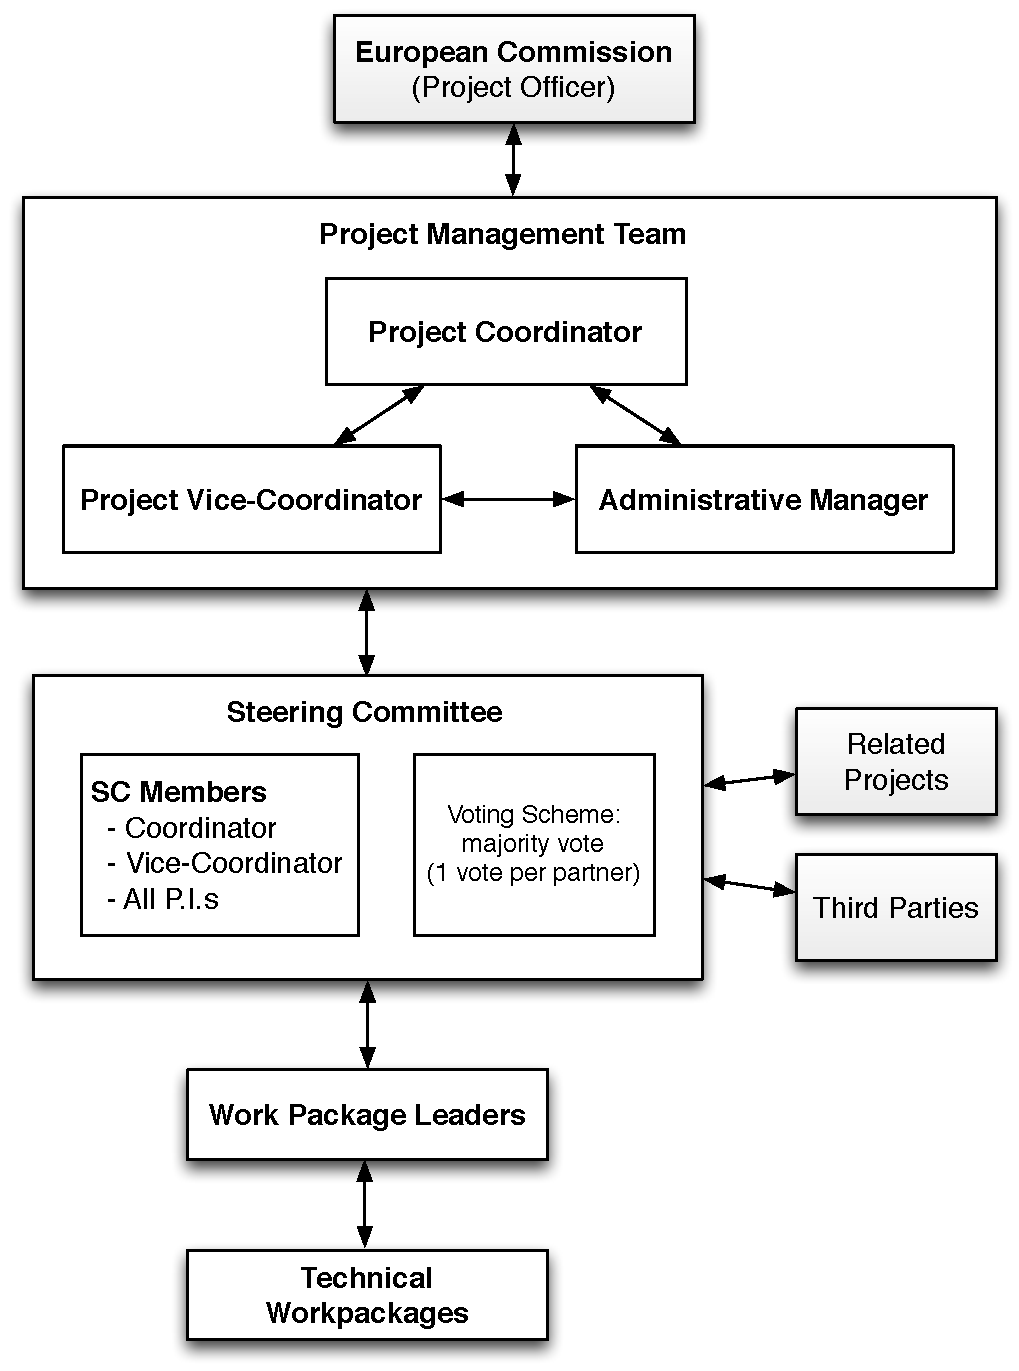
\includegraphics[width=0.4\textwidth]{pics/mngt2}
    \caption{Management scheme for \Project.}
    \label{fig:management}
\end{wrapfigure}

The project management team will
implement clear management processes and promote a qualitative and
dynamic management of all aspects of the project.

The {\em Project Coordinator}, \Coordinator{} from \COORD, has
extensive experience in organizing and supervising international
research projects. He will be
responsible for the overall project strategy, ensuring that all
parties within the consortium know exactly what is expected from them,
as described in the individual work packages.  \Coordinator{} will be
responsible for ensuring that all objectives are met and that all
costs and milestones are in line with the budgets and the provided
Gantt chart. Any deviation will be immediately communicated to the
consortium members and the EC Project Officer.

\Project{} will use the {\em Steering Committee} as a key element of
the project management structure for decision making. It consists of
all PIs, and the Coordinator. The Coordinator will take care of the management of the
project and will ensure the execution of the contract.

\Project{} will be managed and monitored in a clear and effective
manner. It will be organized as depicted in the diagram shown in
Figure~\ref{fig:management}.  In the following, we describe the
individual management structures.



\vspace{3mm}
{\bf The Project Coordinator}


As the Coordinator, \Coordinator{} is the single point of contact
between the European Commission and the consortium.  In this function,
the Coordinator shall:
\begin{denseItemize}
\item Sign the contract with the European Commission
\item Ensure access to the contract by the other contractors
\item Ensure the communication between the consortium and Commission
\item Receive and distribute the EC contribution
\item Collect the cost statements from all contractors for submission
  to the European Commission
\item Prepare, with the support of the consortium, the reports and
  project documents required by the EC %%European Commission
\item Ensure prompt delivery of hardware, software and data
  identified in the contract or requested by the European Commission
  for reviews, including the results of the financial audits prepared
  by independent auditors
\end{denseItemize}

\Coordinator{} will monitor the scientific progress at the
individual partners' sites. He is authorized to execute the project management. Further, he will be accountable to
the project Steering Committee, will be responsible for the
preparation of the Steering Committee meetings and for chairing them.

The following activities belong to the responsibilities of the project
management:
\begin{denseItemize}
  \item The overall legal, contractual, ethical and administrative
  management of the project
  \item Financial management for the Coordinator
  \item Cost calculations for personnel (contracts, time-sheets, \etc), travel, meetings, and equipment (amortization, monitoring of resources)
  \item Juridical advice and administrative advice
  \item Overseeing the promotion of gender equality in the project
  \item Contact management (consortium and EU Project Officer)
  \item Preparing, updating and managing the consortium agreement
    between the participants
  \item Preparing project documents for the Coordinator including
    contracts, meeting minutes, \etc
  \item Decisions on documentation standards
  \item Project Manual for the consortium
  \item Monitoring of important dates and deadlines
  \item Day-to-day management activities
  \item Organization of meetings
  \item Implementation of decisions made by the Coordinator and the
    Steering Committee
  \item Obtaining audit certificates (as and when required) by each of
    the Contractors
  \item Collection of financial reports
  \item Preparation and coordination of project documents such as
    progress and final reports, including Form C, management reports, technical reports, final report, and publishable summary
  \item Supervision of project objectives and timeliness of the work plan
  \item Monitoring and illustration of the project status and data of the partners
  \item Maintaining a project calendar
  \item Management of letters, reminders, transactions
  \item Support the negotiations for late or low-quality activities
\end{denseItemize}


%\vspace{3mm}
{\bf Steering Committee}
\label{sec:mngt:ga}

The \Project{} project has a clear structure and a well-defined
management scheme (see Figure~\ref{fig:management}) with the Steering
Committee as its key decision making instrument.  It is the core
organizational and decision-making body and has the obligation to
ensure that the consortium functions properly.  It will be responsible
for the successful completion of the project and the exploitation of
its results.  It will be chaired by the appointed Project
Coordinator. Further core members of the Steering Committee will
all PIs.  Decisions regarding the project will be made by vote with
each partner having a single vote. A majority of voting members is
required to conduct a meeting (quorum). A simple majority is required
to make formal decisions.  In cases of a tie, the Project Coordinator
will have a casting vote.  Non-voting members and external experts may
be invited by the Chair.

The Steering Committee will normally meet every six months and it
represents the consortium in all related affairs. The duties include,
but are not limited to:
\begin{denseItemize}
\item All budget-related matters
\item The structure and restructuring of the work packages
\item The alteration of the consortium agreement
\item The premature completion / termination of the project
\item Preparation of all documents (financial, reporting, audit, \etc)
\item Management of knowledge
\item Communication between the consortium and the Commission
\item Communication between the consortium and third parties
\item Publicity
\item Establishment and overview of intellectual property procedures
\item Preparation of detailed work plan
\item Steering of the consortium
\end{denseItemize}


\vspace{3mm}
{\bf The Work Package Leaders}

The \Project{} partners will contribute a wide variety of relevant and
sometimes exclusive knowledge, expertise and experience. To ensure the
optimal use of this expertise and to maximize fertile interaction
between partners, work is divided into work packages (WP) each of them
under the responsibility of a WP leader from each of the
partners. Each WP will ultimately be the responsibility of the WP
leader. The WP leaders are responsible for keeping the time schedule
and the appropriate implementation related to their WP. It is also
within their duties to make the necessary contacts with leaders of
other WPs, when their activities depend on the other person's
work. The \Project{} partners will always be informed as to the state
of affairs within every WP.

\vspace{3mm}
{\bf List of Milestones}

The six project milestones described in Section~\ref{sec:milestones} represent a set of quantitative measures for the management to verify the progress of the project. Table~\ref{tab:milestones} on Page~\pageref{tab:milestones} lists the milestones and means of verification.  The time-lines for the milestones and deliverables are presented in the Gantt chart in Figure~\ref{fig:gantt} on Page~\pageref{fig:gantt}.


\subsubsection{Key Project Meetings}
\label{sec:keymeetings}

The Steering Committee will meet at the start of the project and at
six-month intervals. The meetings will normally be scheduled to
rotate between the contractors home base.

The Coordinator will organize these meeting as well as the kick-off
meeting with all partners and the Commission's representative.
The purpose of the project \textbf{kick-off meeting} is to ensure an effective
beginning of the work by detecting and preventing possible problems in
the very beginning such as, for example, delays in the personnel
hiring procedures or device ordering.

%\clearpage
Besides the at least eight \textbf{meetings of the Steering Committee}
throughout the project life-cycle, there will be four
\textbf{integration and testing weeks} to boost the integration
efforts and to perform tests of the overall system. The integration
meetings are scheduled for
\begin{center}
\begin{tabular}{|l|l|}
\hline
\highlightCell Integration and Evaluation Meeting No. & \highlightCell Tentative Schedule \\ \hline\hline
1 (main focus on integration) & M17\\ \hline
2 (main focus on integration and evaluation) & M24\\ \hline
3 (main focus on integration and evaluation) & M41\\ \hline
4 (evaluation) & M48\\ \hline
\end{tabular}
\end{center}

In addition to the above mentioned project meetings, there will be
four \textbf{review meetings} for the project. Here, we follow a time
schedule for EU projects with a duration of 48 months. This results in
four review meetings as shown in the table below.
\begin{center}
\begin{tabular}{|c|l|}
\hline
\highlightCell Review No. & \highlightCell Reviewing Period \\ \hline\hline
1 & M1 -- M12\\ \hline
2 & M13 -- M24\\ \hline
3 & M25 -- M36\\ \hline
4 & M37 -- M48\\ \hline
\end{tabular}
\end{center}



\subsubsection{Management Procedure Tools}

The Coordinator will establish the following
management procedure tools:
\begin{denseItemize}

\item {\bf Project Handbook}: The Coordinator will set up an
  Implementation Strategy, including a the draft of a Project Handbook
  for the purpose of managing information flow, timescales scheduling
  and finance planning as well as best project quality assurance and
  project documentation. This project handbook will be updated as
  appropriate throughout the duration of the project.

\item {\bf Internal assessment}: The Coordinator will
  closely follow and control the progress of the project and the work
  done by each partner.  If the results of this assessment is critical
  or inappropriate, the Coordinator will approach the partner and try
  to help eliminating the problems. If this is not successful, the
  result will be transmitted to the Steering Committee to take
  appropriate actions.

\item {\bf The collaborative platform (Intranet)}: The collaborative
  platform is an Internet-based secured collaborative
  web-site/repository where all project partners can share and
  exchange information. This platform is intended to foster
  collaboration between all partners at all levels: consortium, WP leaders,
  Steering Committee, Coordinator, Project Officer, \etc. Its
  functions include scientific, administrative and financial
  information exchange and archiving. 

\item {\bf Project management software}: The project will use as
  knowledge management software application. The software will ease the financial and technical
  controlling and a constant follow up of the project with key
  performance indicators for an always open project supervision. It
  provides an in-depth view to optimize the work-flow and resource
  allocation in the project.
\end{denseItemize}



\subsubsection{Risks and other Critical Factors}
\label{sec:management:risks_crit_fac}

The consortium will identify the factors that are critical to the
final success of the project and control these factors. For this
purpose, the consortium will define methods and procedures to
identify, assess, monitor and control areas of risk. The challenge
underlying the project has been carefully analyzed. A table of risks
and risk mitigation measures has been included with each {\em work
  package description}. Here we outline project-level risks and our
contingency plans.

%\clearpage

\begin{riskslabeled}{The Cohesiveness of the Consortium}
%%%%%%%%%%%%%%%%%%%%%%%%%%%%%%%%%%%%%%%%%%%%%%%%%%%%%%%%%%%
\item Consortium has no harmony
\putright{ {\em Impact: high, Risk: very low}}

{\em Evaluation:} The partners in the consortium have been carefully
selected, also based on experience with prior collaborations. Multiple
partners already worked together in the EU project V-Charge and other projects. Problems with respect to harmony in the
consortium may arise when the plan of activities is not fully
understood by all participants or when personal incompatibilities
arise during the work. This is very unlikely the case in this proposal
however, since all partners have been intensively involved during the
write-up stage and, in particular, when it came to authoring the parts
for which they bring in their expertise. Thus, all partners are very
well aware of what they committed to.

{\em Resolution:} Previous experiences within the partners have been
very positive and should be maintained at consortium level. In the
very unlikely case of serious conflicts, the conflict resolution
strategies of Section~\ref{sec:confl_mng} will be brought to bear.


%%%%%%%%%%%%%%%%%%%%%%%%%%%%%%%%%%%%%%%%%%%%%%%%%%%%%%%%%%%
\item Poor quality of deliverables
\putright{ {\em Impact: high, Risk: low}}

{\em Resolution:} The Coordinator will monitor the deliverables and
will immediately react in case of low quality. Please note that the
members of the \Project{} consortium are all experienced with
participating in and managing of European research projects, and thus
know the high quality that is expected of the deliverables.



%%%%%%%%%%%%%%%%%%%%%%%%%%%%%%%%%%%%%%%%%%%%%%%%%%%%%%%%%%%
\item Delay in meeting the deadlines
\putright{ {\em Impact: medium, Risk: medium}}

{\em Resolution:} The progress of the project will be assessed at
frequent intervals to predict possible delays and to act
accordingly. The spiral development models allow us to significantly
reduce the risk of delay for components on which others depend.  The
intermediate deliverables developed in the first phase of the spiral
serve as prototypes of software components with limited functionality
will be delivered to the consortium. This also allows us to react
timely in case of upcoming problems and resolve the issues
\emph{before} any critical situation arises. By also controlling if
all partners have successfully started their RTD activities (Milestone
MS1 at M4), the risk of delays in the development is further reduced.
\end{riskslabeled}

%\vspace{5mm}

\begin{riskslabeled}{Technology-Related Problems}

%%%%%%%%%%%%%%%%%%%%%%%%%%%%%%%%%%%%%%%%%%%%%%%%%%%%%%%%%%%
\item The complexity of integration compromises system performance
\putright{ {\em Impact: high, Risk: low}}


{\em Resolution:} Experience of developers is essential to contain this risk. To this end great attention has been devoted during project preparation to the design of clear interfaces between work packages. Any remaining unmodeled interdependencies are expected to be approachable in an effective and timely manner, thanks to the use of the spiral development approach. Furthermore, all members of the
consortium have great experience in large research projects and in the
integration of large and complex systems. Therefore, the likelihood
that such problems will compromise the project is low.


%%%%%%%%%%%%%%%%%%%%%%%%%%%%%%%%%%%%%%%%%%%%%%%%%%%%%%%%%%%
\item Risk plans prepared at the end of each work package may be
  missing important points \putright{ {\em Impact: low, Risk: low}}

{\em Resolution:} To assure that the work packages will be executed
correctly, assessment of the risk plans for each of the work packages
will be made again before they start of the project and updated throughout.

\end{riskslabeled}

\vspace{5mm}


\begin{riskslabeled}{Other Risks}

% %%%%%%%%%%%%%%%%%%%%%%%%%%%%%%%%%%%%%%%%%%%%%%%%%%%%%%%%%%%
 \item Difficulties in handling IPR \putright{ {\em Impact: high, Risk: very low}}

{\em Resolution:} To lower this risk, a consortium agreement will be
 signed before the start of the project.  Furthermore, all partners
 agreed already now on an IPR strategy. The key decisions that are
 formulated in this strategy are summarized in Section~\ref{sec:iprhandling} on
 page~\pageref{sec:iprhandling}. Thus, IPR related issues should not affect the
 developments within the project.
 \end{riskslabeled}




\subsubsection{Conflict Management}
\label{sec:confl_mng}

Conflicts are part of everyday life and occur while working together
in international projects, also for reasons of different cultural
backgrounds. Therefore, possibilities that are available to reduce
conflict potentials will be pursued such as cooperative leadership in
the project and the different working teams. Communication between
consortium members will be facilitated in meetings, telephone and web
conferences so that they get to know each other intensively and
appreciate cultural differences. All project data will be documented
and made available on the shared workspace. If conflicts arise, they
will be firstly internally (by voting) and if necessary externally
solved via mediation techniques (involving a neutral person). In case
of persisting conflicts, the issue will be discussed with the Project
Coordinator who is entitled to overrule all prior voting or moderated
results. In this way, it can be guaranteed that the project is able to
take decisions and function at any time.

Pragmatic negotiation will be the basis for the consortium conflict
resolution approach. Typical conflicts, which can arise in the
project, can be due to a lack of productivity and/or quality, missed
deadlines, different languages and personality or cultural
differences. It will be the responsibility of the Coordinator to identify these
conflicts at an early stage and take steps to talk to the involved
parties to quickly resolve the conflict.  {\em Negotiations} and
decisions taken by consensus will be the main tools to resolve
conflicts.

In case a conflict should arise between the parties, a mediation
procedure shall be started within the consortium. The Coordinator (if
not part of the conflict; should this be the case a neutral
participant of the project will provide to substitute the Coordinator)
will proceed with the following steps:
\begin{denseItemize}
\item Meeting with the conflict parties within one month after being
  officially informed by letter
\item Mediation through an external expert
\item Vote by the Steering Committee
\item European Commission consultation
\item If no other solution is possible devolution to an external court
  of arbitration
\end{denseItemize}

All decision-making procedures and conflict-resolution mechanisms will
be refined and detailed in the consortium agreement.

\subsubsection{Methods of Monitoring and Reporting Progress}

The Steering Committee is an experienced project management team and will
use different methods for monitoring in form of analyses. Each partner is requested to informally report on a
regular basis on progress and deployed resources. In addition to that,
any problems, expected delays, or other events that may impact the
developments in \Project{} have to be reported to the Coordinator as
soon possible.  The documentation standard will be provided by the
Coordinator. All information will be summarized and
distributed to the partners with remarks and countermeasures in case
of major deviations.

All partners will have the responsibility to report to the
Coordinator who has the responsibility to
collect and summarize the reports.  



\subsubsection{Communication Flow}
\label{sec:mngt:comm}
Ensuring a good communication among project partners and towards
outside entities represents an important key of success for the
project and a fundamental practice to manage the project at its best.

The establishment of a fast, reliable and easily accessible
communications infrastructure is vital to the proper operation of a
pan-European project. This can only be achieved through the intensive
use of electronic communications (\eg, email, web based exchanges, Twitter). A
project web-site will also be used to enable fast and efficient
exchanges of information. Thus, main communication channels are
\begin{denseItemize}
\item telephone calls and telephone conferences
\item email
\item web-based services such as internal discussion forums or chats
\item personal meetings
\end{denseItemize}

The internal communication includes physical meetings, starting with a
1-2 day kick-off meeting to guarantee in-depth knowledge exchange.  It
has been planned to have at least six-monthly of the Steering Committee during the project life cycle.  Meetings can also be
accompanied via telephone conferences to discuss project progress and
to take decisions. Also applied are the exchange of emails, letters,
\etc. The advantages of these tools lie in their
functions of allowing the sharing of documents, contact details, white
boards, discussion rooms, \etc. The management team will introduce
such a tool to increase transparency and trust among the project
partners.

The communication flow between \Project{} members will be implemented by:
\begin{denseItemize}
\item Periodic meetings of the Steering Committee
\item Individual working meetings of members of each WP
\item Phone and e-mail interchanges (day to day cooperative working infrastructure)
\end{denseItemize}

The Coordinator has the duty to communicate on a
systematic and frequent basis even if no problems are identified with
every WP leader during the life cycle of their WP to assure the smooth
flow of \Project{} project activities.

All ordinary messages related to a certain work package will be
communicated among all partners involved in that
work package. Nevertheless, any particularly important issues or problems
within the frame of a WP are going to be forwarded to the WP leader
and, if needed, to the Steering Committee.

The experience in running research projects, the good relationships,
and mutual knowledge of the partners as well as their previous
successful collaborations, almost ensures the prevention of problems
regarding communication and information flow within the \Project{} project.


\subsubsection{Statement of Quality}

The \Project{} consortium recognizes that a dedication to quality is
vital to our mission and is essential for delivering
consistent results. Therefore, the consortium agrees on developing a
Statement of Quality with regards to its work.


To achieve its mission, the \Project{} consortium will establish
quality assurance procedures. Underlying these procedures is a set of
principles, which inform the \Project{} Project quality
approach. These are:
\begin{denseItemize}
\item Document procedures, standards and control
\item Issue control for documents
\item Reporting procedures, frequency and format
\item Communication procedures
\item Corrective actions
\item Exception control
\item Conflict resolution
\item Meeting draft agenda
\item Format of meeting minutes
\item Tracking system for actions
\item Specific responsibilities within the project
\end{denseItemize}
\Project{} aims to assure the very highest quality in all the information and analysis it will provide.
All project partners are responsible for quality.  Quality is the
responsibility of every member of the consortium members' staff participating in
the \Project{} project. For the
successful accomplishment of this approach, there are clear lines of
responsibility and accountability for each WP and adequate support to
enable the staff to achieve their quality objectives.  

The \Project{} consortium recognizes that one important factor in assuring
quality is a constant re-examination of our work against the needs
of planned objectives. In this way, we can assure that we are
maintaining appropriate standards and also demonstrate accountability
to the Commission and the public in general of our work. The spiral life cycle approach supports this seamlessly.


\subsubsection{Evaluation Process}

The work progress of the \Project{} Project will be continuously
monitored and supervised by the management team.  In addition to that,
the evaluation meetings (see Section Key Project Meetings on
page~\pageref{sec:keymeetings}) will be carried out to evaluate the
work and progress of the project.

An internal peer review will be performed for each document
produced. Each WP leader will submit all the produced documents to an
appropriate expert internally, not
involved in the same WP, to check for the quality of the documents
produced.

A basis for measuring the quality of the conducted work are the
Measures of Success specified in the work packages descriptions
starting on Page~\pageref{wp1}. Furthermore, the publication of
achieved results in journals as well as European and international
conferences will be taken as a measure of success for the involved
universities and research teams.

Finally, as part of the evaluation process, we will apply a risk
management approach assessing risk in technical, operational and human
resources, the probability that they happen and the impact they will
have in the project. Risks will be reported in the management reports
as well as the actions to reduce the threats and to solve the
situations when these threats materialize.

\subsubsection{Consortium Agreement}

The first task of the Coordinator --  before the project starts -- will be the setup of a consortium
agreement between all the partners. This
procedure will begin immediately after receiving the project approval by the
commission. The consortium agreement will be agreed on and signed
before the beginning of the project.

The consortium agreement will cover the following aspects, as a
minimum:
\begin{denseItemize}
\item The internal organization and management of the consortium
\item Collective Responsibility of the partners
\item Intellectual property arrangements either generated during the
project or existing prior to or acquired in parallel with the project
\item Roles in the consortium
\item Financial viability and audits
\item Exploitation of the project results and commercial considerations
\item Settlement of internal disputes, change in consortium
membership, potential solutions to problems relating to the technical
implementation and solutions to potential financial problems
\end{denseItemize}


\subsubsection{Intellectual Property Handling}%

Intellectual property handling is specified in Section~\ref{sec:iprhandling}, see page~\pageref{sec:iprhandling}.

\subsubsection{Dissemination and Exploitation Activities}%

Details on dissemination and exploitation activities can be found in Section~\ref{sec:diss} on page~\pageref{sec:diss} and in Section~\ref{sec:expl} on page~\pageref{sec:expl}.


% !TEX root = ../proposal.tex

\clearpage
\subsection{Consortium as a whole}
\label{sec:consortium}

% The individual members of the consortium are described in a separate
% section 4. There is no need to repeat that information here. 

% - Describe the consortium. How will it match the projects objectives?
%   How do the members complement one another (and cover the value
%   chain, where appropriate)? In what way does each of them contribute
%   to the project? How will they be able to work effectively together? 
% - If applicable, describe the industrial/commercial involvement in the
%   project to ensure exploitation of the results and explain why this
%   is consistent with and will help to achieve the specific measures
%   which are proposed for exploitation of the results of the project
%   (see section 2.3). 
% - Other countries: If one or more of the participants requesting EU
%   funding is based in a country that is not automatically eligible for
%   such funding (entities from Member States of the EU, from Associated
%   Countries and from one of the countries in the exhaustive list
%   included in General Annex A of the work programme are automatically
%   eligible for EU funding), explain why the participation of the
%   entity in question is essential to carrying out the project 


\subsubsection{Consortium}
%\label{sec:consortium}

The \Project{} consortium consists of five leading partners which fully cover the entire spectrum of know-how necessary to carry out the planned project.  They belong to the technological leaders in their corresponding domains.

Over the past decade, all partners have continuously developed state-of-the art techniques in various areas of robotics and automated driving and all research partners were consortium members of the EUROPA project. Thus, individual partners cooperated already and between them there are overlapping interests. This guarantees that the
interfaces are well understood and at the same time greatly facilitates the collaboration of the individual partners. The integration of these partners in the \Project{} consortium therefore will lead to a substantial synergy effect that will provide innovative solutions to the problems of robot navigation with incomplete map information, navigation in human-populated environments, online semantic scene interpretation, lifelong operation, map handling, sensor calibration, and interaction between people and the robot as well as with other traffic participants such as cars. The following table summarizes the complementary expertise of the involved partners.
%(see also Figure~\ref{fig:puzzle}):

\begin{center}
\small
  \begin{tabular}[h]{|l|p{14cm}|}\hline
    {\highlightCell Partner} & {\highlightCell Expertise}\\\hline\hline
    \VW  & Assisted and automated driving, navigation, data fusion, environment modeling, system integration\\ \hline
    \ETHZ  & Robotics, autonomous cars, calibration, robot navigation, modeling human behavior, system integration \\ \hline
    \IBM  & Cloud deployment, high performance and cognitive computing, analytics  \\ \hline
    \CLUJ & Perception, stereo-vision based perception, detection, tracking, classification, environment representation, scene understanding\\ \hline
    \PRAGUE & TODOCVUT some keywords \\ \hline
  \end{tabular}
\end{center}

The coordinator of the project will be \Coordinator{} from Driver Assistance and Integrated Safety Department at Volkswagen Group Research. In the past, \VW{} has successfully participated in
several European projects listed below. Also the other members of the
consortium have a long history of project participation and thus
experience in carrying out European projects, the subsequent table
shows a list of completed and ongoing EU-funded and other relevant projects.

\begin{center}
\begin{tabular}[h]{|l|p{14cm}|}\hline
    {\highlightCell Partner} & {\highlightCell Previous EU-funded projects}\\\hline\hline
    \VW & V-Charge, AdaptIVe, interactIVe, ARTRAC, HAVEit, euroFOT, INTERSAFE-2
    \\ \hline
    \ETHZ & V-Charge, SHERPA, Flourish, TRADR, EUROPA, EUROPA2
    \\ \hline
    \IBM & NANOSTREAMS, EXA2GREEN, TEXT
    \\ \hline
    \CLUJ & R5-COP, PAN-Robots, DRIVE C2X, INSEMTIVES, LarKC, INTERSAFE-2
	\\ \hline
    \PRAGUE & TODOCVUT 
    \\ \hline
  \end{tabular}
\end{center}

\clearpage
In the \Project{} project, each partner commits knowledge in their core field of expertise leading to the following assignment of contributions. Note that only the key contributions are listed; for a detailed overview, please consult Section~\ref{sec:workpackages}.
\begin{center}
  \begin{tabular}[h]{|l|p{14cm}|}\hline
    {\highlightCell Partner} & {\highlightCell Key contributions in \Project{}}\\\hline\hline
    \VW & vehicle build-up, data fusion and environment representation, navigation, integration, management of the project
    \\ \hline
    \ETHZ & Accurate all-time metric localization; lifelong large-scale mapping; map management and map summarization.
    \\ \hline
    \IBM & cloud infrastructure; software deployment and test infrastructure; knowledge representation and maintenance; analytics
    \\ \hline
    \CLUJ & 360 degrees redundant perception solution based on available or new 2D and 3D sensors and on the spatio-temporal and appearance based low level representation; Robust algorithms necessary for perception adaptation to adverse visibility conditions, road infrastructure perception, real time 3D terrain perception, road user perception and signaling perception; Object level multi-sensor fusion that allows perception refinement offering an increased robustness and accuracy of the detection, tracking and classification methods.
    \\ \hline
	\PRAGUE & Algorithms for scene understanding, exploiting the perception and data fusion from heterogeneous sensor set, 3D terrain perception
    \\ \hline
 \end{tabular}
\end{center}


\subsubsection{Sub-Contracting}
\label{sec:subcontracting}
Subcontracting will not be used in the project.


\subsubsection{Other Countries}
The Swiss consortium members \ETHZ, and \IBM{} are considered under the category ''industrialised third country'' for Industrial Leadership submissions. As such they do not request funding from the EC (see Figure~\ref{fig:budgetoverview}, on page~\pageref{fig:budgetoverview}). If the proposal is selected, the Swiss members of the \Project{} project will receive funding from the Swiss government directly.



%--------------------------------------------


\subsection{Resources to be committed}
\label{sec:resources}
\subsubsection{Budget overview}
The majority of the requested budget is caused by personnel expenses. The university partners will mainly
employ Ph.D. students and postdocs to carry out the work described above, while the industrial partners employ technical experts and experienced scientists. The detailed personnel cost and claimed person months for Ph.D. students, postdocs, technical experts, and senior personnel is shown in Figure~\ref{fig:budgetoverview}. The
figure shows the budget broken down in detail, including the direct personnel and other direct costs.
Beside the personnel cost, the partners request between \euro30K and \euro48K for travel costs. This includes
travels to different sites, primarily for the four consortium wide integration weeks to carry out test trials and for data collection and mapping, travels to meetings, conference,
as well as partner exchanges.
Furthermore, budget is allocated for equipment/consumables for the partners. The allocated components differ among the
individual partners, as replicating a full car at all partners' sites would be too expensive and is also
not needed to conduct the project. Two automated vehicle platforms and a cloud infrastructure will be needed within \Project{}. One vehicle will
be located at \VW{} at all times, while the other one will be shared among the other partners. The project intends on re-using one of the cars from the V-Charge project and for that one \VW{} only requests funding for extensions and modifications. \IBM requests equipment funding for the cloud infrastructure that will be required for the computation, maintenance and deployment of the lifelong map as well as learning for scene understanding. While both the vehicles as well as the cloud appear on the budget of single partners, these platforms truly enable the project and serve the entire consortium.
 The other partners only allocate resources for equipment in order to build a sensor platform, or for a mockup platform for the individual tasks at the partners' sites in order to conduct their developments. More details can be found below in the individual budgets of the partners.

\begin{figure}[h]
  \caption{Budget overview.}
  \centering
    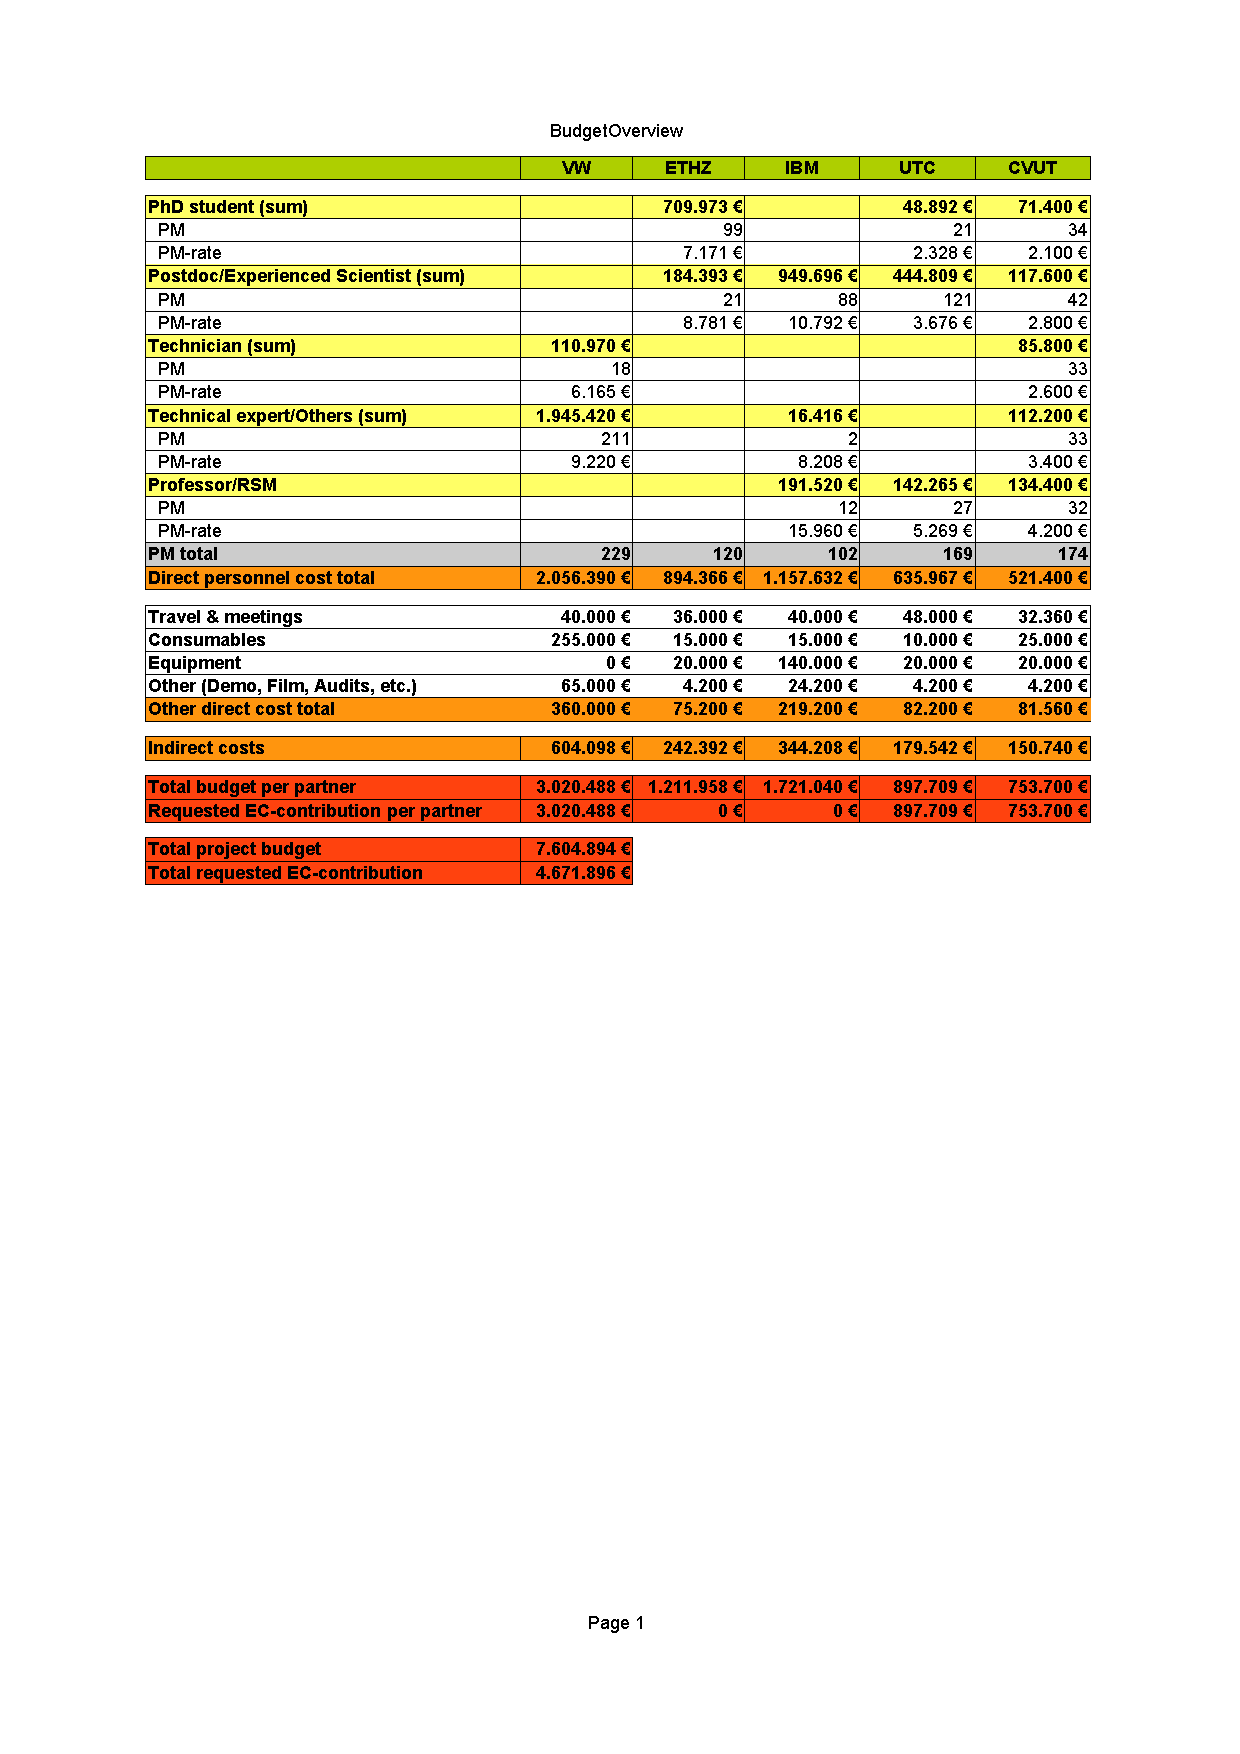
\includegraphics[trim=2cm 13cm 2cm 2.45cm, clip=true, width=0.9\textwidth]{pics/UP-Drive_Budget.pdf}
   \label{fig:budgetoverview}
\end{figure}


\subsubsection{Partner-specific justification for resources}

\ETHZ requests 120 PMs over the project lifetime on RTD activities. This corresponds to 2 Ph.D. students 
with 48 and 51 PMs, respectively, and a postdoc with 21 PMs. The Ph.D. students and the postdoc will work
on the localization and mapping framework within the project, with one student focusing on online localization, the other on offline mapping. Both will be involved in the integration and testing efforts. The postdoc will oversee this work and focus on integration, testing, 
and dissemination activities. Note that the contribution for \ETHZ (\euro 1,211,958) will be provided by Switzerland so that no EC contribution 
is needed for \ETHZ. 

\VW will devote 229 PMs over the project lifetime for RTD and management activities. 140 PMs will be split almost evenly between the areas: perception, navigation and integration + the associated tasks of specification and dissemination. This corresponds to 3 technical experts working full-time on their respective fields throughout the project. The adaptation and build-up of the two vehicles will be prepared and validated by an technical expert and performed by technicians, resulting in an effort of 24 and 18 PMs in the respective cost-categories. Additional 22 PMs will be devoted to scene understanding. Project coordination will require 25 PMs. Apart from the personnel costs \VW will also have substantial Consumable costs (\euro 255,000) which will be devoted to equipping the vehicles with sensor systems, computer hardware, safety elements and other items necessary to complete the test and demonstration platforms. Regarding other costs, \VW expects \euro 50,000 costs for the organization of the final demonstration with press representatives as well as further \euro 15,000 for items such as project logo, press materials and audit. In total \VW requests a contribution from the EC of \euro 3,020,487.50. For a tabular view, please consult Figure~\ref{fig:budgetoverview}.

\IBM will devote 88 PMs for an experienced scientist, two PMs for a technical expert and 12 PMs for the principal investigator over the project lifetime on RTD and management activities.
The total PM count for experienced scientists will be divided into three positions. The first one, in conjunction with the technical expert, will be in charge of the hardware and cloud infrastructure buildup. The second one will work on the software deployment functionality and map management. The third one will mainly be involved in scene understanding. The P.I. will guide and manage these roles and conduct research on mapping and scene understanding. He further focuses on integration, testing, 
and dissemination activities. \IBM in addition needs \euro 140,000 for cloud infrastructure acquisition forming a crucial part of the project. While forming part of the budget of \IBM, the infrastructure will be extensively used by all project partners for computation, storage and communication activities, particularly lifelong mapping and learning for scene understanding. A further \euro 20,000 are needed to compose a project film for dissemination purposes. For a tabular view, please consult Figure~\ref{fig:budgetoverview}. Note that the contribution for \IBM (\euro 1,721,040) will be provided by Switzerland so that no EC contribution is needed for \IBM. 

\CLUJ requests 169 PMs over the project lifetime for RTD activities. This
corresponds to 1 PhD student with 21 PMs, 5 post-doc with approx. 24 PMs
each and 1 professor with 27 PMs. The PhD student and 4 postdocs will
work on requirements, data acquisition and development of perception
algorithms. One postdoc will work on scene understanding tasks. The
professor will supervise all the work and focus on integration,
dissemination and management activities. \CLUJ requests a total contribution from the EC of \euro 897,709.

\PRAGUE requests 174 PMs over the project lifetime on RTD and project management activities. TODOCVUT... explain the use of ressources \PRAGUE requests a total contribution from the EC of \euro 753,700.
%\input{text/section3Resources}


\clearpage

%\bibliographystyle{plainsmall} %TODO: make this work to densify the bib

\bibliographystyle{plain}
\bibliography{bib/projectBib,bib/unipr,bib/ethz,bib/utc}

\clearpage

\end{document}
